% Options for packages loaded elsewhere
\PassOptionsToPackage{unicode}{hyperref}
\PassOptionsToPackage{hyphens}{url}
\documentclass[
  10pt,
  letterpaper,
  openany]{report}
\usepackage{xcolor}
\usepackage[margin=0.72in,headheight=14pt]{geometry}
\usepackage{amsmath,amssymb}
\setcounter{secnumdepth}{5}
\usepackage{iftex}
\ifPDFTeX
  \usepackage[T1]{fontenc}
  \usepackage[utf8]{inputenc}
  \usepackage{textcomp} % provide euro and other symbols
\else % if luatex or xetex
  \usepackage{unicode-math} % this also loads fontspec
  \defaultfontfeatures{Scale=MatchLowercase}
  \defaultfontfeatures[\rmfamily]{Ligatures=TeX,Scale=1}
\fi
\usepackage{lmodern}
\ifPDFTeX\else
  % Match the HTML system-ui typeface on macOS after lmodern initializes
  % the fallback text and math fonts used by generated LaTeX constructs.
  \setmainfont{SFNS.ttf}[
    Path=/System/Library/Fonts/,
    BoldFont=SFNS.ttf,
    BoldFeatures={FakeBold=1.5},
    ItalicFont=SFNSItalic.ttf,
    BoldItalicFont=SFNSItalic.ttf,
    BoldItalicFeatures={FakeBold=1.5}]
  \setsansfont{SFNS.ttf}[
    Path=/System/Library/Fonts/,
    BoldFont=SFNS.ttf,
    BoldFeatures={FakeBold=1.5},
    ItalicFont=SFNSItalic.ttf,
    BoldItalicFont=SFNSItalic.ttf,
    BoldItalicFeatures={FakeBold=1.5}]
\fi
% Use upquote if available, for straight quotes in verbatim environments
\IfFileExists{upquote.sty}{\usepackage{upquote}}{}
\IfFileExists{microtype.sty}{% use microtype if available
  \usepackage[]{microtype}
  \UseMicrotypeSet[protrusion]{basicmath} % disable protrusion for tt fonts
}{}
\makeatletter
\@ifundefined{KOMAClassName}{% if non-KOMA class
  \IfFileExists{parskip.sty}{%
    \usepackage{parskip}
  }{% else
    \setlength{\parindent}{0pt}
    \setlength{\parskip}{6pt plus 2pt minus 1pt}}
}{% if KOMA class
  \KOMAoptions{parskip=half}}
\makeatother
\usepackage{longtable,booktabs,array}
\usepackage{caption}
\captionsetup[table]{skip=6pt}
\newcounter{none} % for unnumbered tables
\usepackage{calc} % for calculating minipage widths
% Correct order of tables after \paragraph or \subparagraph
\usepackage{etoolbox}
\makeatletter
\patchcmd\longtable{\par}{\if@noskipsec\mbox{}\fi\par}{}{}
\makeatother
% Allow footnotes in longtable head/foot
\IfFileExists{footnotehyper.sty}{\usepackage{footnotehyper}}{\usepackage{footnote}}
\makesavenoteenv{longtable}
\usepackage{graphicx}
\makeatletter
\newsavebox\pandoc@box
\newcommand*\pandocbounded[1]{% scales image to fit in text height/width
  \sbox\pandoc@box{#1}%
  \Gscale@div\@tempa{\textheight}{\dimexpr\ht\pandoc@box+\dp\pandoc@box\relax}%
  \Gscale@div\@tempb{\linewidth}{\wd\pandoc@box}%
  \ifdim\@tempb\p@<\@tempa\p@\let\@tempa\@tempb\fi% select the smaller of both
  \ifdim\@tempa\p@<\p@\scalebox{\@tempa}{\usebox\pandoc@box}%
  \else\usebox{\pandoc@box}%
  \fi%
}
% Set default figure placement to htbp
\def\fps@figure{htbp}
\makeatother
\setlength{\emergencystretch}{3em} % prevent overfull lines
\providecommand{\tightlist}{%
  \setlength{\itemsep}{0pt}\setlength{\parskip}{0pt}}
\usepackage{booktabs,longtable,array,graphicx,float,caption,enumitem,fancyhdr,titlesec,xcolor,tcolorbox}
\tcbuselibrary{breakable}
\definecolor{MarsNavy}{HTML}{17384F}
\definecolor{MarsBlue}{HTML}{24577A}
\definecolor{MarsMuted}{HTML}{506878}
\definecolor{MarsOrange}{HTML}{E87318}
\definecolor{MarsLine}{HTML}{D6E0E6}
\definecolor{MarsNotice}{HTML}{EAF3F8}
\definecolor{MarsWarn}{HTML}{FFF2DA}
\definecolor{MarsDanger}{HTML}{FFE3E1}
\definecolor{MarsSafe}{HTML}{E6F5EB}
\setkeys{Gin}{width=\linewidth,height=.72\textheight,keepaspectratio}
\captionsetup{font={small,color=MarsMuted},labelfont=bf,textfont={},skip=6pt}
\setlist{leftmargin=*,itemsep=4pt,topsep=5pt}
\setlength{\parindent}{0pt}
\setlength{\parskip}{5pt}
\setlength{\LTpre}{6pt}
\setlength{\LTpost}{10pt}
\renewcommand{\arraystretch}{1.16}
\emergencystretch=3em
\raggedbottom
\setcounter{tocdepth}{1}
\setcounter{secnumdepth}{2}
\titleformat{\chapter}[display]
  {\normalfont\bfseries\color{MarsNavy}}
  {\filleft\Large\color{MarsOrange}\chaptername\ \thechapter}
  {8pt}{\Huge}
\titlespacing*{\chapter}{0pt}{-20pt}{24pt}
\titleformat{\section}{\Large\bfseries\color{MarsNavy}}{\thesection}{.65em}{}
\titleformat{\subsection}{\large\bfseries\color{MarsBlue}}{\thesubsection}{.65em}{}
\pagestyle{fancy}
\fancyhf{}
\fancyhead[L]{\small MARS RC Robot System}
\fancyhead[R]{\small\nouppercase{\leftmark}}
\fancyfoot[C]{\thepage}
\renewcommand{\headrulewidth}{0.4pt}
\renewcommand{\headrule}{\hbox to\headwidth{\color{MarsLine}\leaders\hrule height \headrulewidth\hfill}}
\newtcolorbox{manualnotice}{breakable,colback=MarsNotice,colframe=MarsBlue,boxrule=.6pt,leftrule=4pt,arc=2mm,left=7pt,right=7pt,top=6pt,bottom=6pt}
\newtcolorbox{manualwarning}{breakable,colback=MarsWarn,colframe=MarsOrange,boxrule=.6pt,leftrule=4pt,arc=2mm,left=7pt,right=7pt,top=6pt,bottom=6pt}
\newtcolorbox{manualdanger}{breakable,colback=MarsDanger,colframe=red!75!black,boxrule=.6pt,leftrule=4pt,arc=2mm,left=7pt,right=7pt,top=6pt,bottom=6pt}
\newtcolorbox{manualsafe}{breakable,colback=MarsSafe,colframe=green!50!black,boxrule=.6pt,leftrule=4pt,arc=2mm,left=7pt,right=7pt,top=6pt,bottom=6pt}
\AtBeginEnvironment{longtable}{\small}
\AtBeginDocument{\hypersetup{colorlinks=true,linkcolor=MarsBlue,urlcolor=MarsBlue,citecolor=MarsBlue,pdfborder={0 0 0}}}
\usepackage{bookmark}
\IfFileExists{xurl.sty}{\usepackage{xurl}}{} % add URL line breaks if available
\urlstyle{same}
% fallback for those not using the hyperref driver hyperxmp:
\makeatletter
\@ifundefined{xmpquote}{\newcommand{\xmpquote}[1]{#1}}{}
\makeatother
\hypersetup{
  pdftitle={MARS RC Robot System},
  hidelinks,
  pdfcreator={LaTeX via pandoc}}

\title{MARS RC Robot System}
\usepackage{etoolbox}
\makeatletter
\providecommand{\subtitle}[1]{% add subtitle to \maketitle
  \apptocmd{\@title}{\par {\large #1 \par}}{}{}
}
\makeatother
\subtitle{Operation, Safety, Service, and Maintenance Manual}
\author{}
\date{August 2026}

\begin{document}
\maketitle

{
\setcounter{tocdepth}{2}
\tableofcontents
}
\chapter{Start here}\label{start-here}

\protect\phantomsection\label{start}
\section{Before first use}\label{before-first-use}

\begin{manualdanger}

\textbf{This machine can move unexpectedly and uses hazardous UV-C
light.} A trained adult must supervise it. Keep the physical emergency
stop within reach. UV-C can injure eyes and skin; operate the lamps only
after establishing and controlling a field exclusion zone, posting
warnings, confirming remote supervision, and verifying every installed
safety device.

\end{manualdanger}

\subsection{What a non-technical operator must
know}\label{what-a-non-technical-operator-must-know}

\begin{itemize}
\tightlist
\item
  \textbf{Hold} means the robot is commanded not to move.
\item
  \textbf{Manual} means a handheld joystick controls movement.
\item
  \textbf{Auto} means the navigation controller follows an uploaded
  route.
\item
  \textbf{RTK} is the precise GPS state needed for accurate navigation.
\item
  \textbf{Arm} prepares UVC control; it must not turn the lamps on.
\item
  \textbf{All Off} and \textbf{Disarm} are required before anyone enters
  the UV-C area.
\end{itemize}

\subsection{First-use checklist}\label{first-use-checklist}

\begin{enumerate}
\tightlist
\item
  Read every component chapter before operating the system.
\item
  Identify the physical emergency stop and test it with UVC power
  disconnected.
\item
  Attach every radio and GPS antenna before switching equipment on.
\item
  Test driving with the wheels raised or the robot otherwise restrained.
\item
  Test the UVC relay with safe indicator loads before connecting UV-C
  lamps.
\item
  Run the first automatic mission in a large empty area at low speed.
\end{enumerate}

\protect\phantomsection\label{system}
\section{Robot system overview}\label{robot-system-overview}

The handheld controller, mobile robot, RTK GPS, navigation controller,
power hub, UVC relay, inverters, ballasts, and lamps work together as
shown in Figure~\ref{fig:system-component-overview}.

\begin{figure}
\centering
\pandocbounded{
\includegraphics[keepaspectratio,alt={Complete controller, robot, GPS, relay, UVC, and navigation connection map}]{assets/system-component-map.pdf}}
\caption{The controller commands the robot. The GPS base corrects the
robot rover. The navigation controller uses corrected position and its
camera for supervised automatic navigation. The robot master controls
motion and all six UVC relay channels.}
\label{fig:system-component-overview}
\end{figure}

{Component}

\subsection{RC controllers}\label{rc-controllers}

Handheld manual control, robot status, and Dual Joystick Remote
Controller RTK-correction reception.

{Component}

\subsection{Mobile robot and UVC}\label{mobile-robot-and-uvc}

Drive, steering, batteries, CAN relay, inverters, ballasts, and four
lamps.

{Component}

\subsection{RTK GPS}\label{rtk-gps}

Fixed base plus rover receiver on the robot.

{Component}

\subsection{Navigation controller}\label{navigation-controller}

Raspberry Pi 5 computer, CSI-connected Pi camera, PoE power module, web
console, and route planning.

\subsection{Robot views}\label{robot-views}

Figures~\ref{fig:robot-rear-view}--\ref{fig:robot-side-view} identify
the robot orientation, major external components, and service
compartments from the rear, front, and side.

\begin{figure}
\centering
\pandocbounded{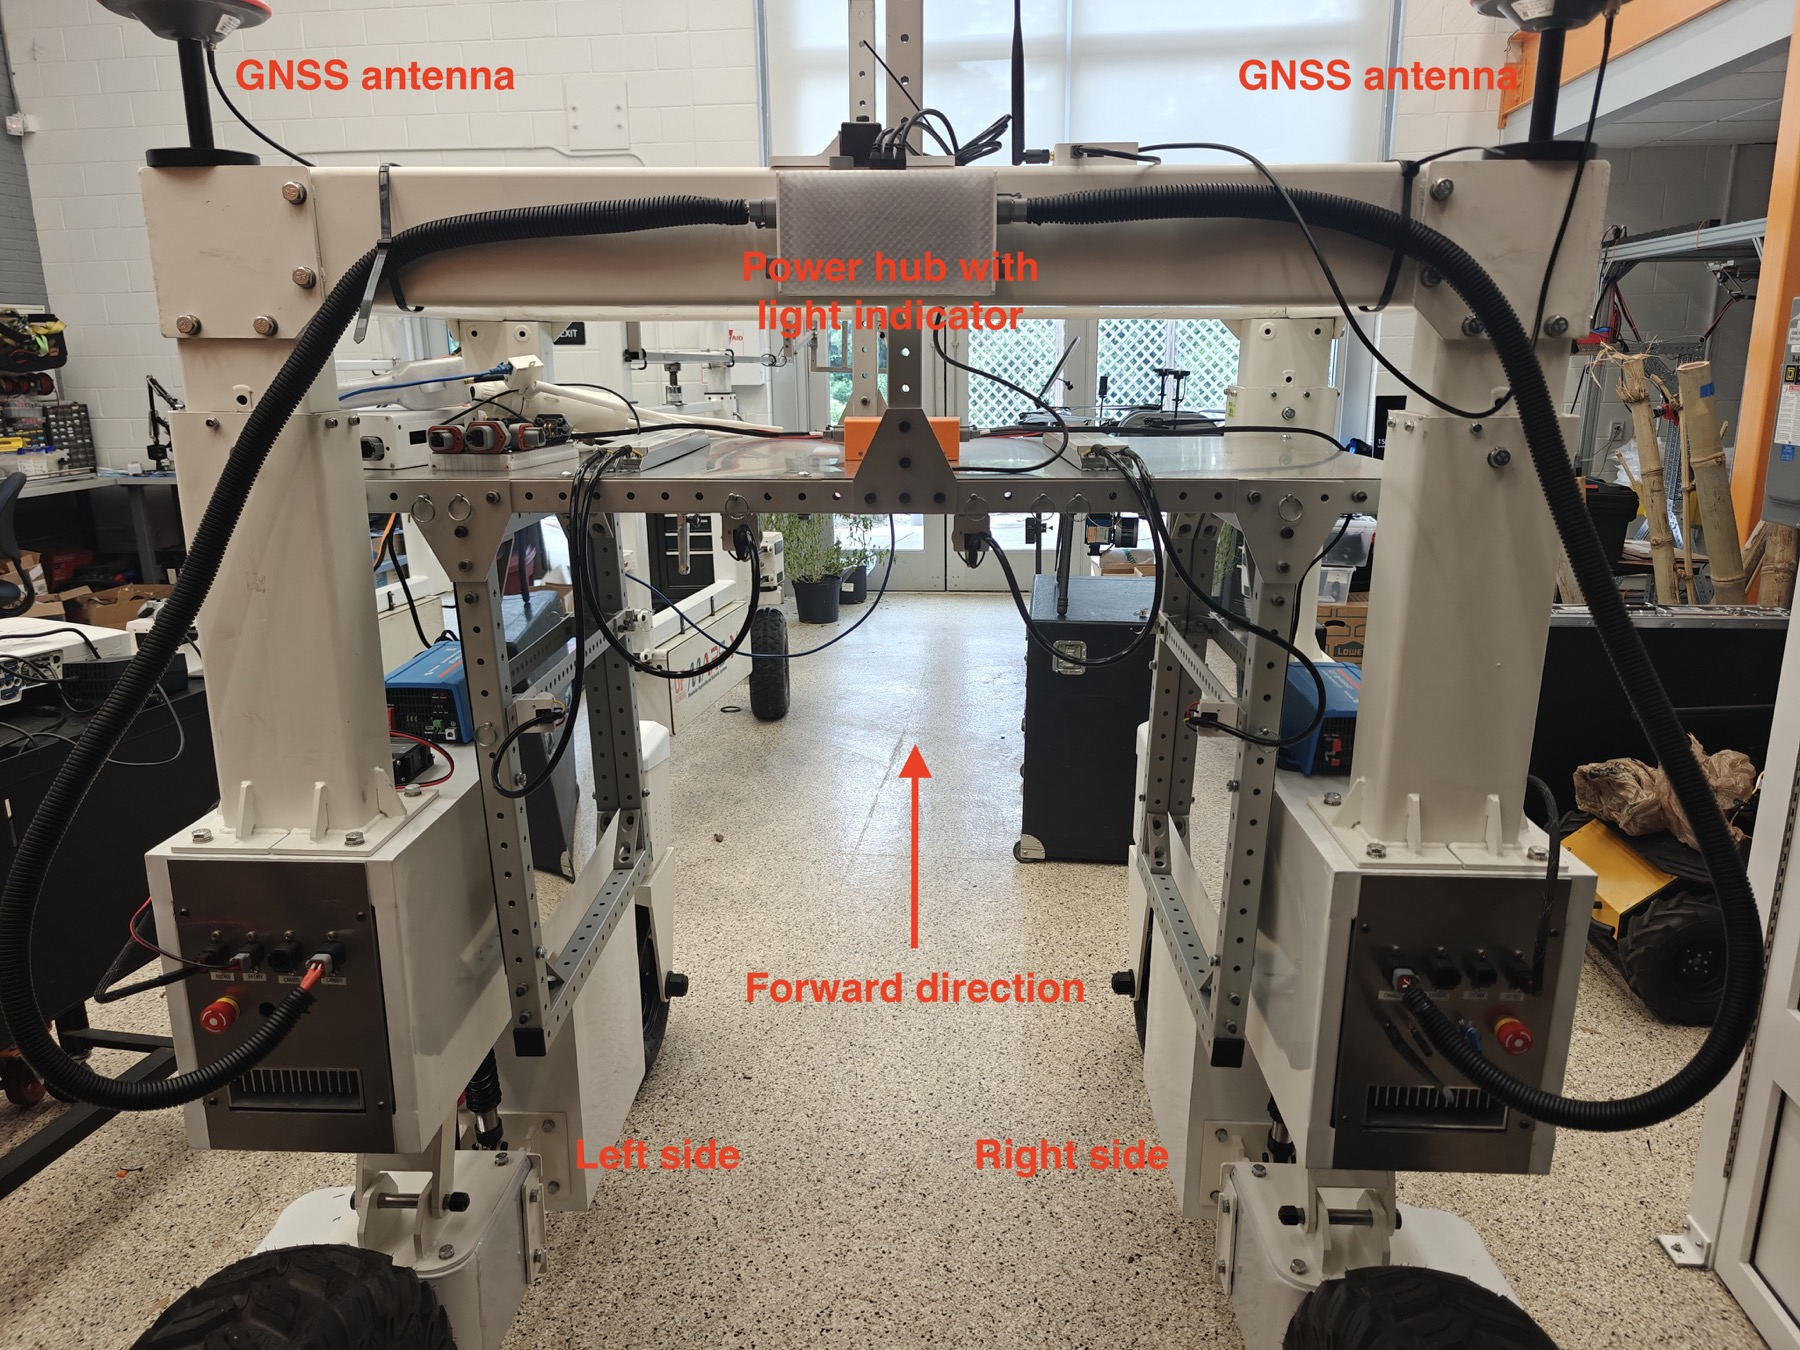
\includegraphics[keepaspectratio,alt={Rear view of the mobile robot showing both GNSS antennas, left and right sides, forward direction, and the power hub light indicator}]{assets/robot-rear-view.jpg}}
\caption{Rear view: the labels identify the left and right sides,
forward direction, two GNSS antennas, and the power hub with its light
indicator.}
\label{fig:robot-rear-view}
\end{figure}

\begin{figure}
\centering
\pandocbounded{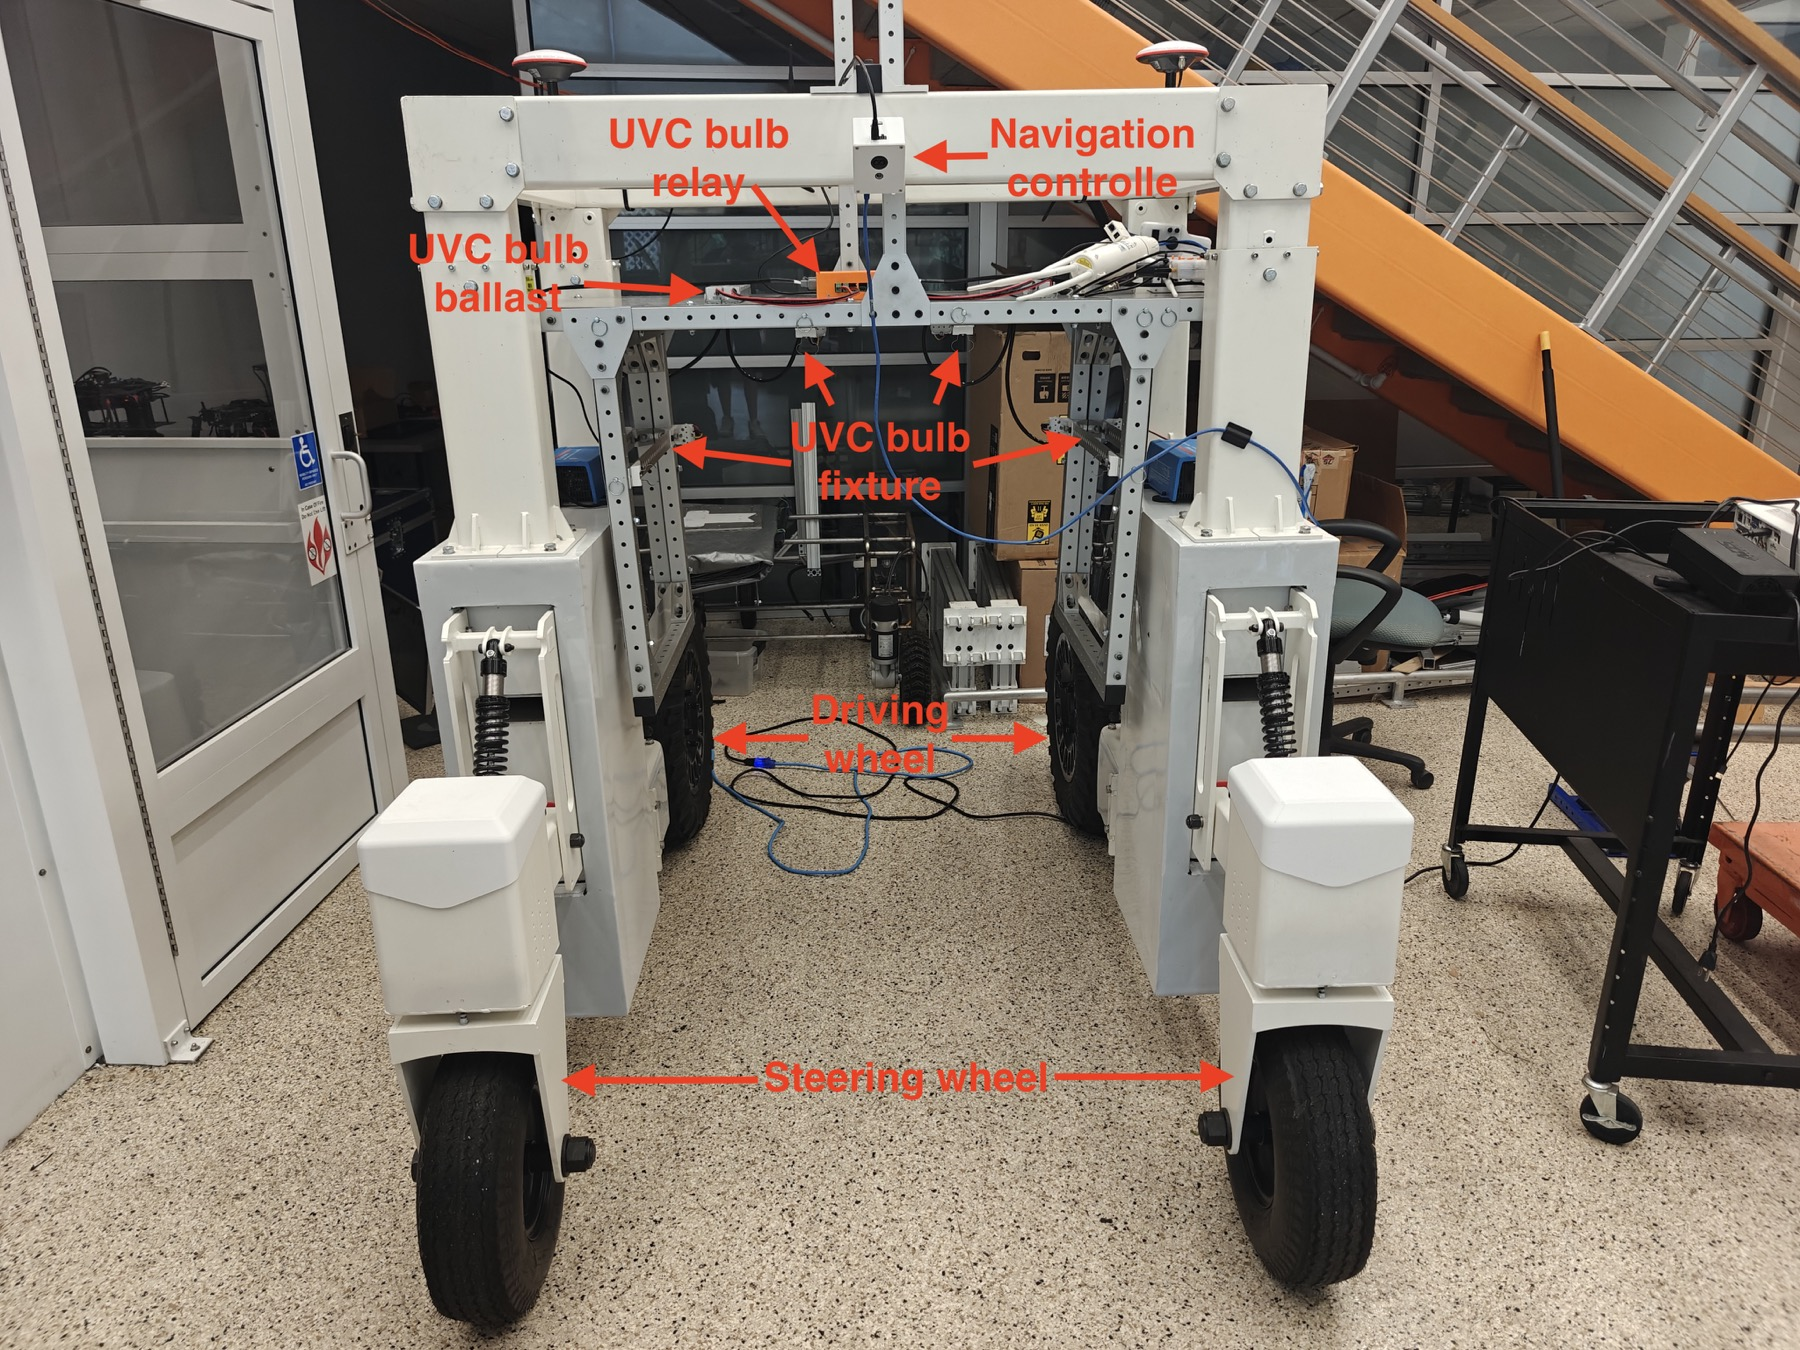
\includegraphics[keepaspectratio,alt={Front view of the mobile robot showing steering and driving wheels, UVC fixtures, ballast, relay, and navigation controller}]{assets/robot-front-view.jpg}}
\caption{Front view: the steering wheels are at the front; the labeled
equipment includes the driving wheels, UVC fixtures, UVC ballast and
relay, and navigation controller.}
\label{fig:robot-front-view}
\end{figure}

\begin{figure}
\centering
\pandocbounded{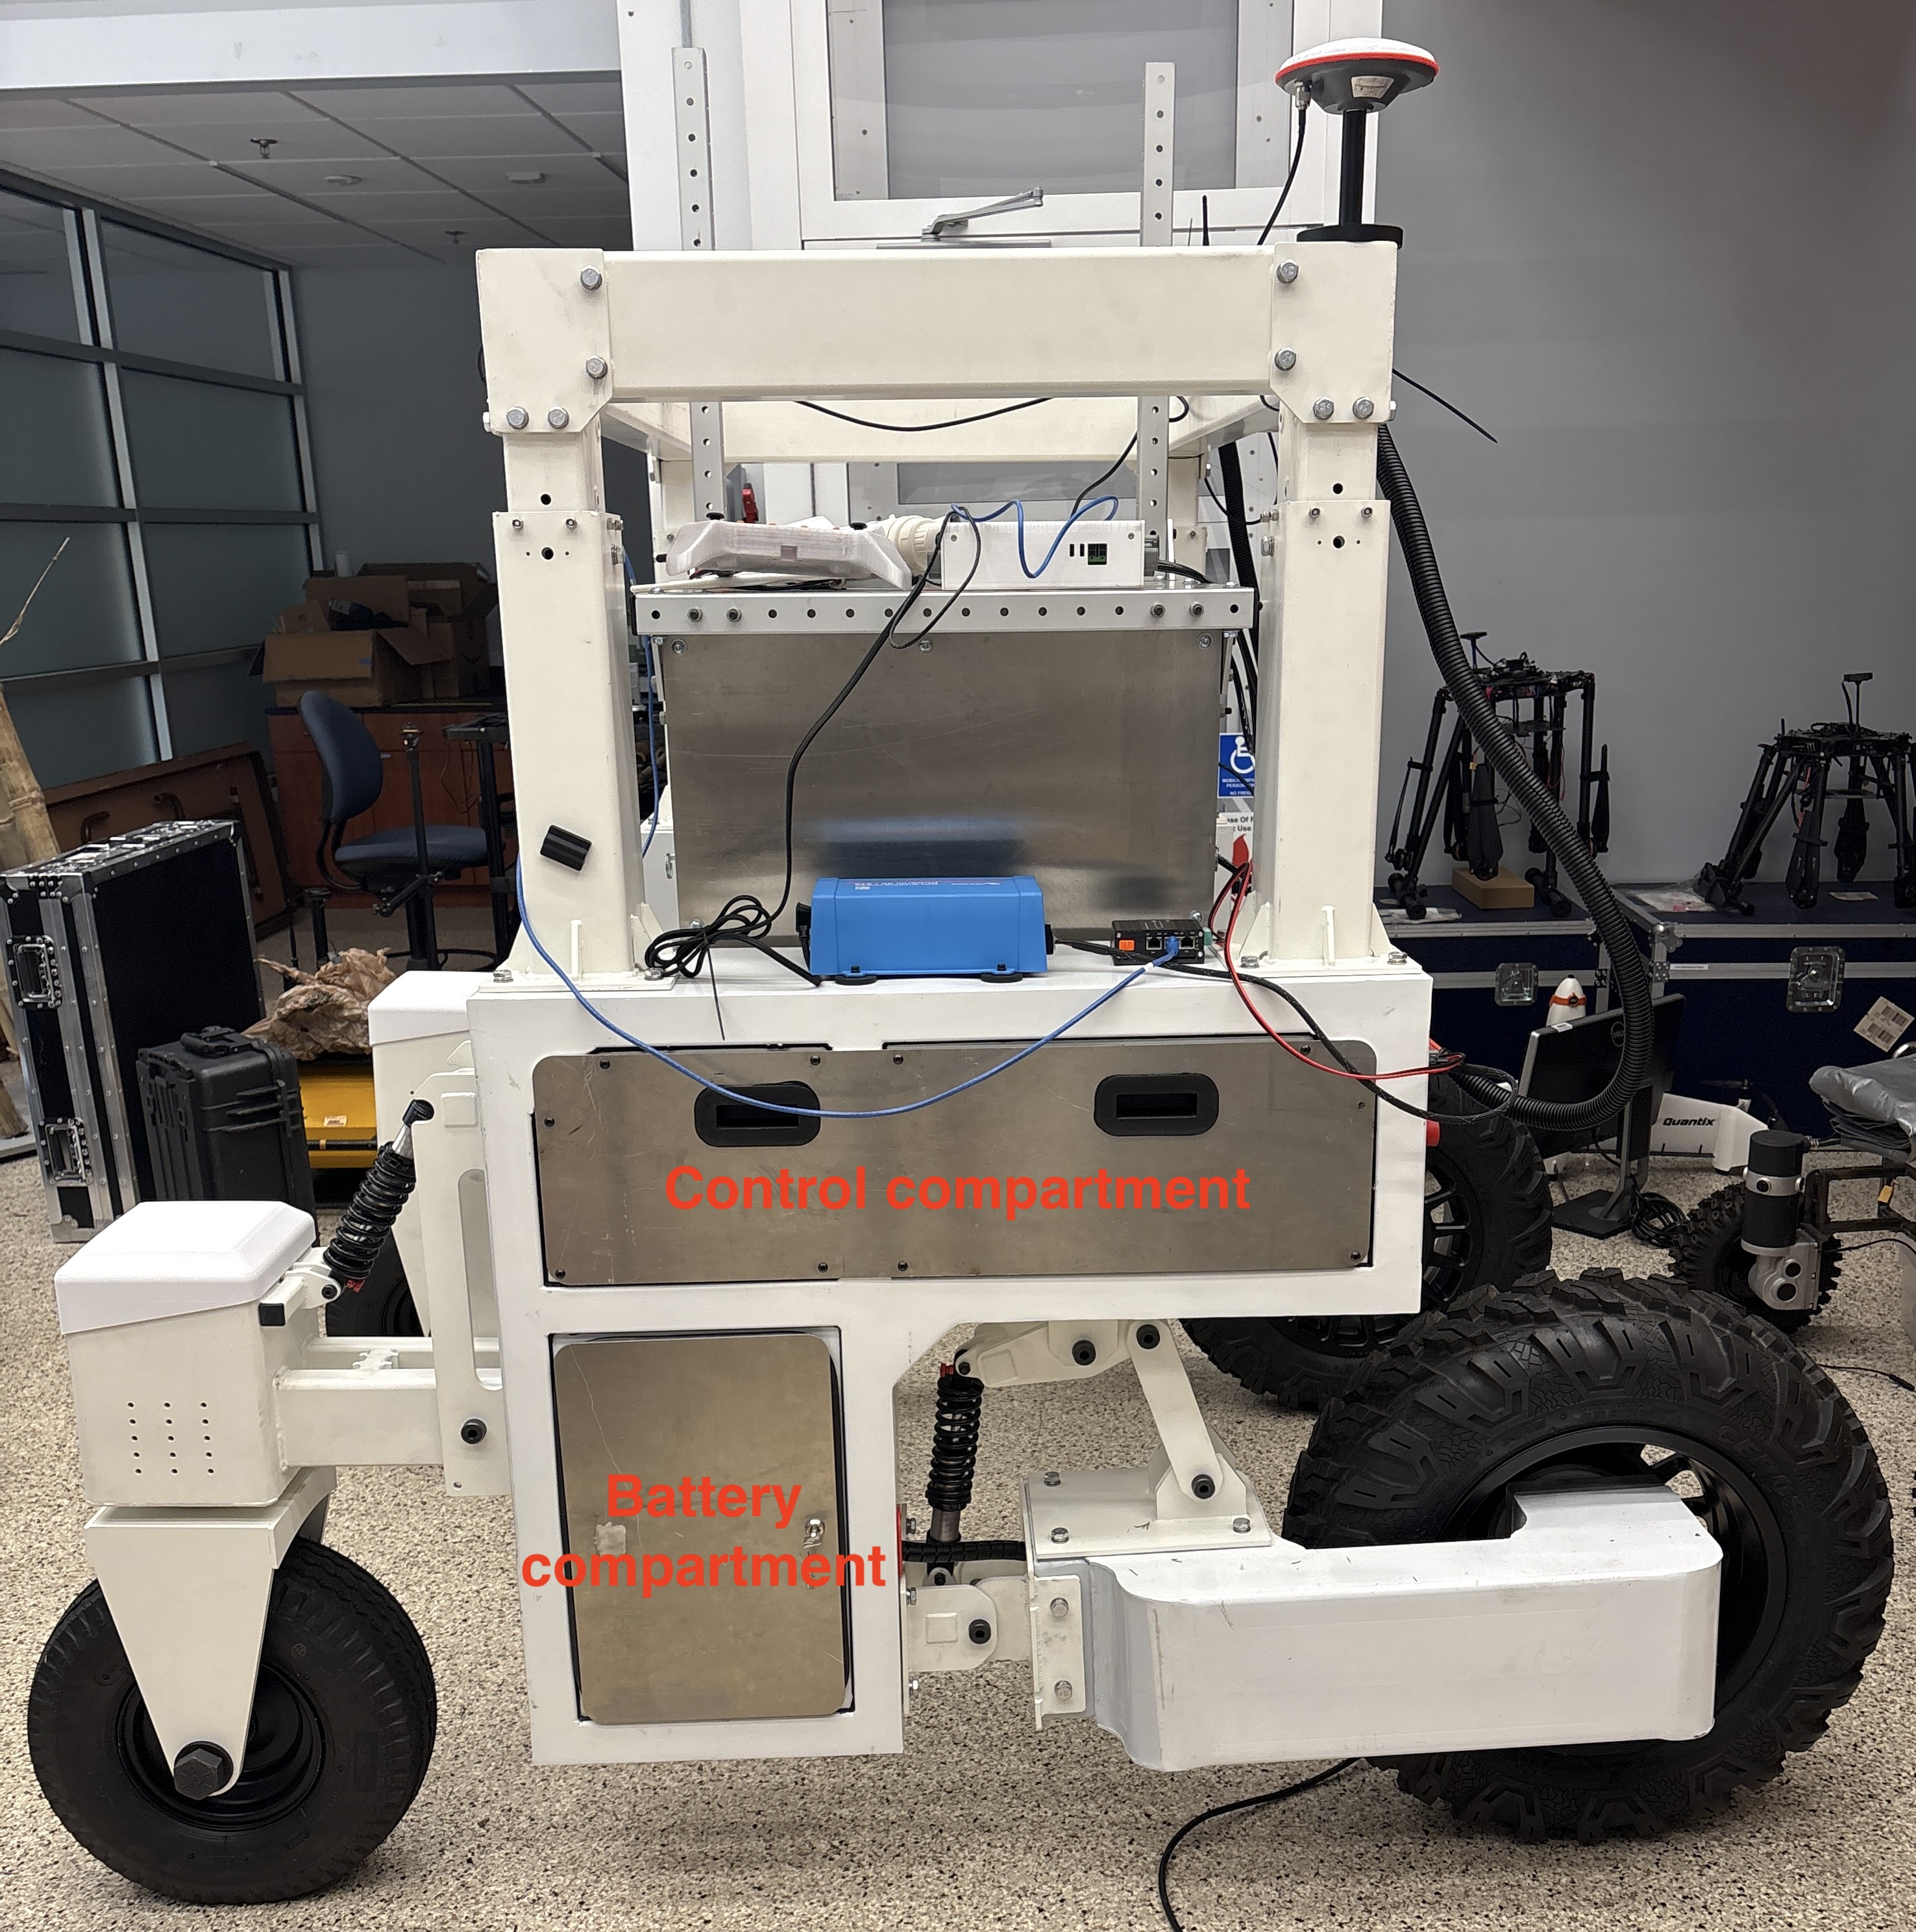
\includegraphics[keepaspectratio,alt={Side view of the mobile robot showing its steering wheel, driving wheel, controller compartment, battery compartment, frame, and GNSS antenna}]{assets/robot-side-view.jpg}}
\caption{Side view: the labeled controller and battery compartments are
positioned between the steering wheel and the larger driving wheel.}
\label{fig:robot-side-view}
\end{figure}

\subsection{Inside the controller
compartments}\label{inside-the-controller-compartments}

Figures~\ref{fig:controller-compartment-controls} and
\ref{fig:controller-compartment-power} identify the control, switching,
and high-current components inside the controller compartments.

\begin{figure}
\centering
\pandocbounded{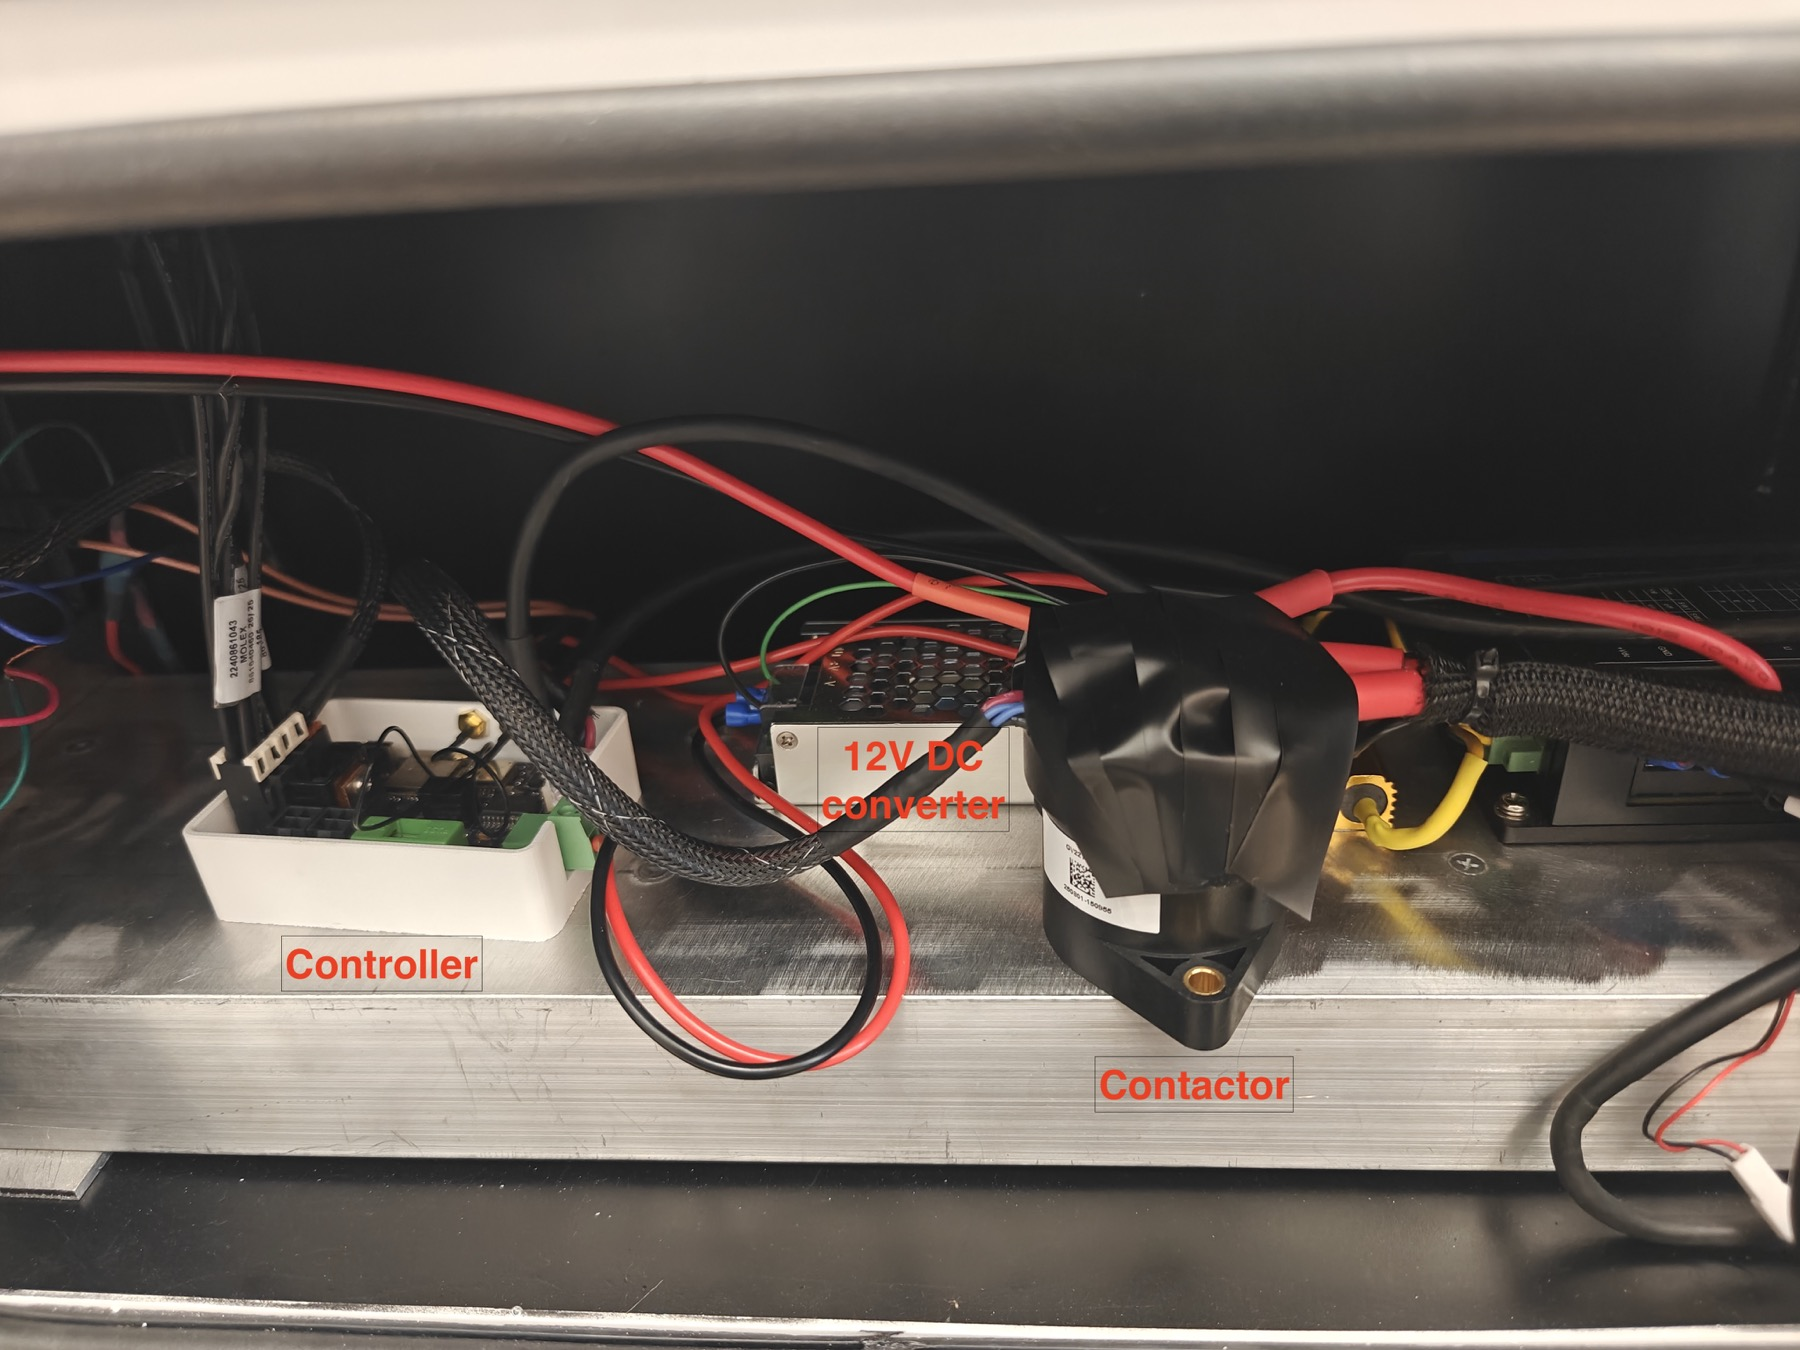
\includegraphics[keepaspectratio,alt={Inside a robot controller compartment showing the robot controller, 12 volt DC converter, contactor, and wiring}]{assets/robot-controller-compartment-controls.jpg}}
\caption{Control and switching components inside the compartment: robot
controller, 12 V DC converter, main contactor, and associated wiring.}
\label{fig:controller-compartment-controls}
\end{figure}

\begin{figure}
\centering
\pandocbounded{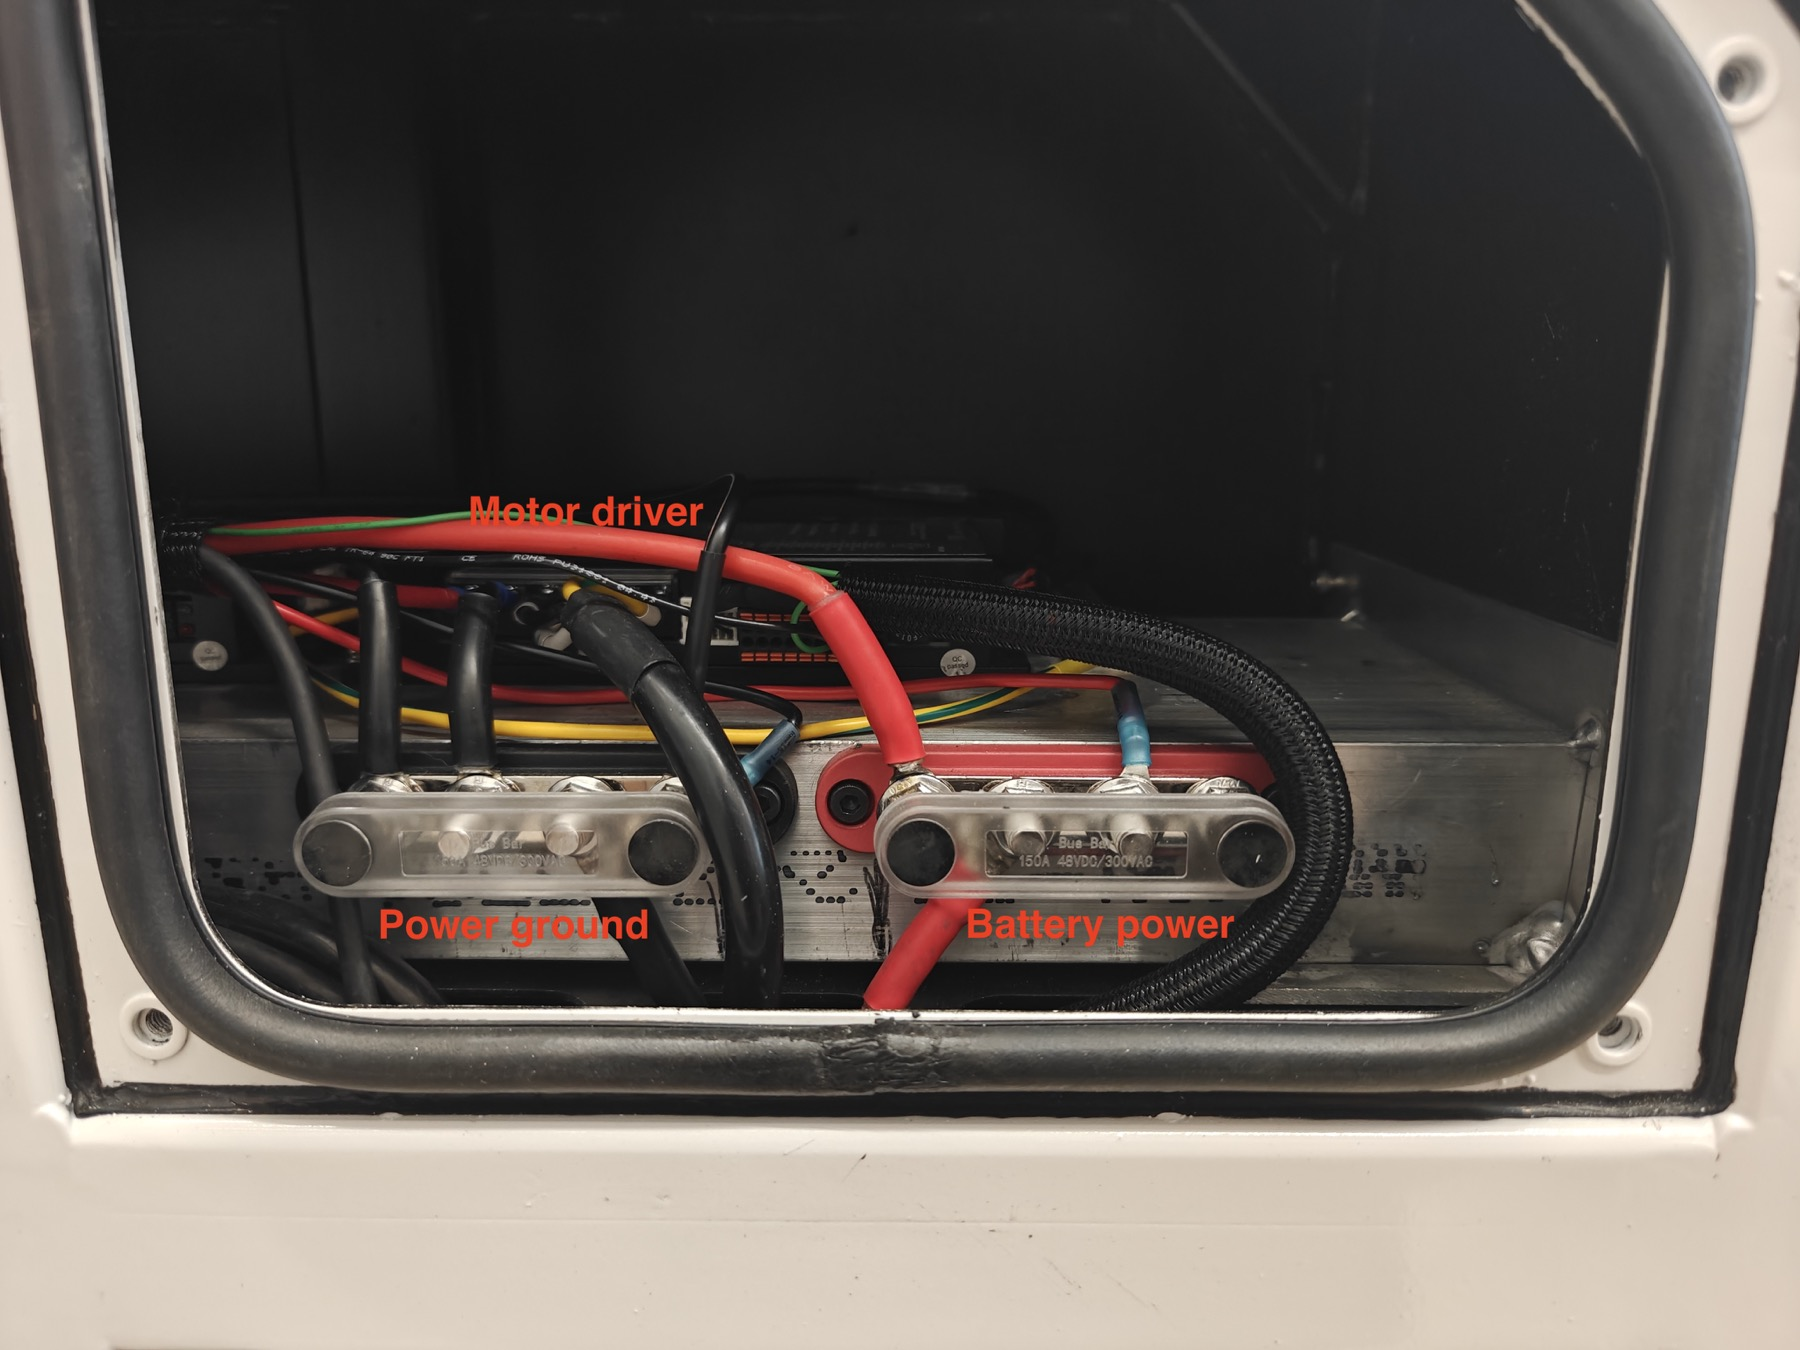
\includegraphics[keepaspectratio,alt={Inside a robot controller compartment showing the motor driver, battery-power busbar, power-ground busbar, and high-current cables}]{assets/robot-controller-compartment-power.jpg}}
\caption{Motor-power components inside the compartment: motor driver,
battery-power busbar, power-ground busbar, and high-current cabling.}
\label{fig:controller-compartment-power}
\end{figure}

\begin{manualwarning}

\textbf{Controller compartments contain high-current electrical
equipment.} Operators should keep the covers closed. Qualified service
personnel must switch the robot off, isolate both batteries, verify the
contactor is open, and follow the site lockout procedure before opening
or touching internal components.

\end{manualwarning}

\protect\phantomsection\label{system-diagrams}
\section{Robot system diagrams}\label{robot-system-diagrams}

This page is the visual index for the system. Each caption links to the
detailed instructions kept with the related component.

\subsection{1 · System architecture}\label{system-architecture}

Figure~\ref{fig:system-architecture} summarizes the information and
power relationships among the major robot-system components.

\begin{figure}[H]
\centering
\pandocbounded{
\includegraphics[keepaspectratio,alt={MARS robot system component architecture}]{assets/system-component-map.pdf}}
\caption{RC controllers, mobile robot/UVC, RTK base and rover, and
navigation controller. See \hyperref[system]{system overview} and
\hyperref[operations]{complete-system operations}.}
\label{fig:system-architecture}
\end{figure}

\clearpage
\subsection{2 · Physical power, network, radio and CAN
connections}\label{physical-power-network-radio-and-can-connections}

Figure~\ref{fig:physical-connections} traces the installed power,
network, radio, and CAN connections.

\begin{figure}[H]
\centering
\pandocbounded{
\includegraphics[keepaspectratio,alt={Whole robot physical power network radio and CAN wiring diagram}]{assets/system-physical-can-layout.pdf}}
\caption{Shows the robot chassis, four motors, cross-chassis power hub,
PoE path, RTK/RC radios and UVC AC path. See
\hyperref[system-connections]{physical connection schedule} and
\hyperref[robot-connections]{robot side ports}.}
\label{fig:physical-connections}
\end{figure}

\clearpage
\subsection{3 · Power-hub ports and device power
paths}\label{power-hub-ports-and-device-power-paths}

Figure~\ref{fig:power-hub-paths} identifies the power-hub ports and the
devices powered through each group.

\begin{figure}[H]
\centering
\pandocbounded{
\includegraphics[keepaspectratio,alt={Power hub 12 volt and 5 volt CAN and power ports with GPS rover UVC relay and navigation connections}]{assets/power-hub-port-map.pdf}}
\caption{The GNSS rover and UVC relay receive 5 V and CAN from the hub.
The navigation controller uses a 5 V CAN hub port for communication but
receives operating power through PoE. See the
\hyperref[power-hub-ports]{power-hub port schedule},
\hyperref[gps-connections]{GPS connections}, and
\hyperref[nav-connections]{navigation connections}.}
\label{fig:power-hub-paths}
\end{figure}

\clearpage
\subsection{4 · CANopen topology and object
ranges}\label{canopen-topology-and-object-ranges}

Figure~\ref{fig:canopen-topology} shows the installed CANopen nodes and
their principal object ranges.

\begin{figure}[H]
\centering
\pandocbounded{
\includegraphics[keepaspectratio,alt={CANopen topology and object ranges for every robot CAN device}]{assets/canopen-object-map.pdf}}
\caption{Installed bus is 500 kbit/s; motor nodes are 1--4. See
\hyperref[canopen-objects]{CANopen dictionaries} and
\hyperref[power-hub-objects]{power-hub objects}.}
\label{fig:canopen-topology}
\end{figure}

\clearpage
\subsection{5 · Power-on state flow}\label{power-on-state-flow}

Figure~\ref{fig:power-on-flow} shows the expected startup sequence and
the corresponding power-hub LED states.

\begin{figure}[H]
\centering
\pandocbounded{
\includegraphics[keepaspectratio,alt={Robot precharge contactor CAN homing and ready state flow}]{assets/robot-power-on-led-guide.pdf}}
\caption{Expected precharge, contactor sound, CAN checks, steering
homing, ready state and LED changes. See
\hyperref[robot-startup]{power-on behavior} and
\hyperref[power-hub-led]{LED meanings}.}
\label{fig:power-on-flow}
\end{figure}

\clearpage

\protect\phantomsection\label{system-connections}
\section{How the complete robot system is
connected}\label{how-the-complete-robot-system-is-connected}

This section is the connection overview for the whole product. The blue
dashed paths are radios, green is Ethernet/PoE, red is switched battery
power, orange is UVC AC power, and brown is CAN. A CAN node ID
identifies electronics on the bus; it is not a connector number.

\begin{figure}
\centering
\pandocbounded{
\includegraphics[keepaspectratio,alt={Physical wiring, radio links, CAN backbone, power paths, and CAN node IDs for the complete robot system}]{assets/system-physical-can-layout.pdf}}
\caption{The installed motor nodes are 1--4, the power hub/status LED is
node 14, the GNSS rover uses a powered 5 V CAN port, and the navigation
controller has separate CAN and PoE connections.}
\end{figure}

\begin{manualwarning}

\textbf{Connection rule:} keep power Off and the contactor open while
making connections. Match the printed port label and voltage. Power-hub
CAN ports may place either \textbf{12 V or 5 V on pin 1}; both use pin 2
CANH, pin 3 CANL and pin 4 GND. They are not interchangeable.

\end{manualwarning}

\subsection{Physical connection
schedule}\label{physical-connection-schedule}

{\def\LTcaptype{none} % do not increment counter
\begin{longtable}[]{@{}
  >{\raggedright\arraybackslash}p{(\linewidth - 6\tabcolsep) * \real{0.2500}}
  >{\raggedright\arraybackslash}p{(\linewidth - 6\tabcolsep) * \real{0.2500}}
  >{\raggedright\arraybackslash}p{(\linewidth - 6\tabcolsep) * \real{0.2500}}
  >{\raggedright\arraybackslash}p{(\linewidth - 6\tabcolsep) * \real{0.2500}}@{}}
\toprule\noalign{}
\begin{minipage}[b]{\linewidth}\raggedright
From
\end{minipage} & \begin{minipage}[b]{\linewidth}\raggedright
To
\end{minipage} & \begin{minipage}[b]{\linewidth}\raggedright
Physical link
\end{minipage} & \begin{minipage}[b]{\linewidth}\raggedright
Purpose and check
\end{minipage} \\
\midrule\noalign{}
\endhead
\bottomrule\noalign{}
\endlastfoot
Single Joystick Remote Controller or Dual Joystick Remote Controller &
Robot master receiver & RC LoRa radio & Manual commands and robot
telemetry use MAVLink 2, with one complete MAVLink frame in each RC LoRa
packet. The RC settings must match the robot. \\
RTK base & Robot rover; Dual Joystick Remote Controller RTK receiver
when used & RTK LoRa radio & Correction data. It must match the base and
must not reuse the RC LoRa settings. \\
Robot CAN backbone & Master controller, slave controller, motor nodes
1--4, GNSS rover, UVC relay, power hub/LED, and navigation CAN interface
& CANH, CANL and common GND; hub ports provide labelled 12 V or 5 V &
Commands, status, position, relay control, heartbeats, and faults. See
the \hyperref[power-hub-ports]{power-hub port schedule}. \\
Each robot side & External CAN accessories & Two CAN ports per side: 12
V, GND, CANH, CANL & The two ports are bus connection points, not four
separate CAN node IDs. Use short stubs and the approved port
assignment. \\
Power-hub 5 V CAN port & GNSS rover & 5 V, CANH, CANL and GND & The
rover receives both operating power and CAN communication through this
connection. \\
Power-hub 5 V CAN port & UVC relay, node 15 & 5 V, CANH, CANL and GND &
The relay electronics receive 5 V operating power and CAN communication
through this connection. Its isolated relay contacts switch the ballast
AC inputs; the 5 V supply never powers a lamp or ballast. \\
Power-hub 5 V CAN port & Navigation controller & Installed 5 V CAN-port
connection: pin 1 = 5 V, pin 2 = CANH, pin 3 = CANL, pin 4 = GND & The
navigation controller connects to the assigned 5 V CAN port for its
robot CAN connection. Its main operating power and Ethernet connection
come from the robot PoE switch. Do not modify the installed harness. \\
Robot battery through protected branch & Robot PoE switch & DC power &
Powers the network switch; verify its rated input and branch
protection. \\
Robot PoE switch & Navigation-controller external PoE port & PoE
Ethernet cable & Provides the navigation controller\textquotesingle s
operating power and Ethernet network connection. \\
Robot battery through contactor & Two battery-power ports on each side &
Switched DC & Accessory power. Verify voltage and polarity before
attaching equipment. \\
48 V battery & Two Victron inverters & Protected DC & One inverter
supplies each robot side. \\
Inverters & Relay AC inputs -\textgreater{} four ballasts
-\textgreater{} four lamps & 120 V AC & Relay node 15 switches each
ballast input. One ballast serves one lamp. \\
\end{longtable}
}

\subsection{CAN node schedule}\label{can-node-schedule}

{\def\LTcaptype{none} % do not increment counter
\begin{longtable}[]{@{}
  >{\raggedright\arraybackslash}p{(\linewidth - 6\tabcolsep) * \real{0.2500}}
  >{\raggedright\arraybackslash}p{(\linewidth - 6\tabcolsep) * \real{0.2500}}
  >{\raggedright\arraybackslash}p{(\linewidth - 6\tabcolsep) * \real{0.2500}}
  >{\raggedright\arraybackslash}p{(\linewidth - 6\tabcolsep) * \real{0.2500}}@{}}
\toprule\noalign{}
\begin{minipage}[b]{\linewidth}\raggedright
Component
\end{minipage} & \begin{minipage}[b]{\linewidth}\raggedright
Decimal
\end{minipage} & \begin{minipage}[b]{\linewidth}\raggedright
Hex
\end{minipage} & \begin{minipage}[b]{\linewidth}\raggedright
Segment / role
\end{minipage} \\
\midrule\noalign{}
\endhead
\bottomrule\noalign{}
\endlastfoot
Steering motor 1 & 1 & \texttt{0x01} & Steering axis; homed during
startup. \\
Steering motor 2 & 2 & \texttt{0x02} & Steering axis; homed during
startup. \\
Drive motor 1 & 3 & \texttt{0x03} & Velocity-controlled drive axis. \\
Drive motor 2 & 4 & \texttt{0x04} & Velocity-controlled drive axis. \\
Right/slave robot controller & 10 & \texttt{0x0A} & Right/slave CAN
controller. \\
Left/master robot controller & 11 & \texttt{0x0B} & Robot master and
target of navigation velocity/status bridge. \\
Power hub and status LED & 14 & \texttt{0x0E} & Connects both robot
sides and displays robot startup, running, idle, link and safety
states. \\
UVC relay & 15 & \texttt{0x0F} & Powered from a power-hub 5 V CAN port;
controls all six relay channels. \\
Robot GNSS rover & 20 & \texttt{0x14} & Corrected position;
web-configurable, firmware default shown. \\
RTK base CAN interface & 21 & \texttt{0x15} & Base firmware default;
normally the field base is remote and is not physically attached to the
robot CAN bus. \\
Navigation controller &
\multicolumn{2}{>{\raggedright\arraybackslash}p{(\linewidth - 6\tabcolsep) * \real{0.5000} + 2\tabcolsep}}{%
\textbf{No separate CANopen node ID}} & SocketCAN client/bridge on
\texttt{can0}; targets robot node 11 and observes node 10. \\
Handheld controllers, PoE switch, inverters, ballasts, lamps &
\multicolumn{2}{>{\raggedright\arraybackslash}p{(\linewidth - 6\tabcolsep) * \real{0.5000} + 2\tabcolsep}}{%
\textbf{Not CAN nodes}} & Radio, Ethernet/power, or switched AC
equipment. \\
\end{longtable}
}

\begin{manualnotice}

\textbf{Installed CAN setting:} every device on the robot CAN segment
must use \textbf{500 kbit/s}. Read each configurable
device\textquotesingle s live node ID, compare it with the as-built
record, and verify that every active node is unique. The table documents
firmware defaults and the current robot configuration; an authorized
node-ID change can make a live value different.

\end{manualnotice}

\subsection{CAN cable and termination
checks}\label{can-cable-and-termination-checks}

\begin{enumerate}
\tightlist
\item
  Open the contactor and isolate UVC AC power.
\item
  Verify the connector label and pinout before mating it; never probe by
  wire color alone.
\item
  Maintain the approved CAN trunk with short stubs. Keep CAN wiring
  separated from inverter, ballast, motor-power, and lamp wiring.
\item
  With all CAN power Off, measure approximately 60 Ω between CANH and
  CANL on a correctly terminated bus. A substantially different reading
  requires wiring/termination inspection before energizing.
\item
  Check common ground continuity, CANH/CANL polarity, shield/ground
  practice, cable strain relief, the power-hub cross-chassis connection,
  and the two end terminators.
\item
  Set every attached CAN device to \textbf{500 kbit/s}. Energize in
  Hold. Confirm motor nodes 1--4, slave node 10, master node 11, power
  hub node 14, relay node 15 and rover node 20 are unique and producing
  expected heartbeats without bus errors before enabling motion, Auto
  navigation, or UVC.
\end{enumerate}

\protect\phantomsection\label{canopen-objects}
\section{CANopenNode object
dictionaries}\label{canopennode-object-dictionaries}

This is the field-engineer reference for the objects implemented by the
installed software release. The robot bus operates at \textbf{500
kbit/s}. Index and subindex are hexadecimal; for example,
\texttt{0x2013:02} means object \texttt{0x2013}, subindex 2.

\begin{figure}
\centering
\pandocbounded{
\includegraphics[keepaspectratio,alt={CANopen object dictionary map for every CAN device on the 500 kilobit robot bus}]{assets/canopen-object-map.pdf}}
\caption{Application objects are in the manufacturer-specific
\protect\texttt{0x2000} range. Motor drives additionally use the CiA 402
drive profile. The navigation controller is a SocketCAN client/bridge
and has no object dictionary or CANopen node ID.}
\end{figure}

\begin{manualdanger}

\textbf{Engineering access only:} an SDO or PDO write can move the
robot, release steering, alter safety timing, or energize all six UVC
relay channels. Put the robot in Hold, restrain the wheels, disconnect
UVC AC power, preserve the original EDS/XDD and parameter backup, and
obtain authorization before writing. Operators should use the normal
controller and webpages, not raw CANopen writes.

\end{manualdanger}

\subsection{Notation and common communication
objects}\label{notation-and-common-communication-objects}

\textbf{RO} = read-only; \textbf{RW} = read/write; \textbf{WO} =
write-only; \textbf{TPDO} = transmitted process data; \textbf{RPDO} =
received process data. For arrays, subindex \texttt{00} is the RO
element count and data begins at subindex \texttt{01}.

{\def\LTcaptype{none} % do not increment counter
\begin{longtable}[]{@{}
  >{\raggedright\arraybackslash}p{(\linewidth - 4\tabcolsep) * \real{0.3333}}
  >{\raggedright\arraybackslash}p{(\linewidth - 4\tabcolsep) * \real{0.3333}}
  >{\raggedright\arraybackslash}p{(\linewidth - 4\tabcolsep) * \real{0.3333}}@{}}
\toprule\noalign{}
\begin{minipage}[b]{\linewidth}\raggedright
Index or range
\end{minipage} & \begin{minipage}[b]{\linewidth}\raggedright
CANopenNode object
\end{minipage} & \begin{minipage}[b]{\linewidth}\raggedright
Field use
\end{minipage} \\
\midrule\noalign{}
\endhead
\bottomrule\noalign{}
\endlastfoot
\texttt{0x1000}, \texttt{0x1001}, \texttt{0x1003} & Device type, error
register, pre-defined error field & Identify the node and diagnose
active/history errors. Read before clearing faults. \\
\texttt{0x1005–0x1007}, \texttt{0x1019} & SYNC COB-ID, cycle period,
synchronous window, counter overflow & Timing configuration. Do not
change on one node alone. \\
\texttt{0x1008–0x100A} & Device name, hardware version, software version
& Present in the GNSS dictionaries; use for asset/firmware records. \\
\texttt{0x1010}, \texttt{0x1011} & Store parameters, restore defaults &
Controlled service commands. Back up first; restart may be required. \\
\texttt{0x1012}, \texttt{0x1014}, \texttt{0x1015} & Time-stamp COB-ID,
EMCY COB-ID, EMCY inhibit time & Emergency and time-stamp
communication. \\
\texttt{0x1016}, \texttt{0x1017} & Consumer and producer heartbeat times
& Node-loss supervision. Never lengthen a safety heartbeat without
revalidating the system. \\
\texttt{0x1018} & Identity record & Vendor ID, product code, revision
and serial number where populated. \\
\texttt{0x1200}, \texttt{0x1280} & SDO server and SDO client parameters
& Configuration/diagnostic channel. Normal default SDO COB-IDs are
\texttt{0x600\ +\ node} request and \texttt{0x580\ +\ node} response. \\
\texttt{0x1400…}, \texttt{0x1600…} & RPDO communication and mapping &
Defines received real-time data. The robot master implements
\texttt{0x1400–0x140C}/\texttt{0x1600–0x160C}. \\
\texttt{0x1800…}, \texttt{0x1A00…} & TPDO communication and mapping &
Defines transmitted real-time data. Master: six TPDOs; slave: one;
rover: six; base: eight. \\
\end{longtable}
}

\subsection{Robot master node 11 and robot slave node
10}\label{robot-master-node-11-and-robot-slave-node-10}

The following application objects are common to both robot-controller
dictionaries unless marked otherwise. Arrays \texttt{0x2008},
\texttt{0x2009}, \texttt{0x200F}, \texttt{0x2012}, \texttt{0x2014}, and
\texttt{0x201F–0x2024} use subindices \texttt{01–04} for four
axes/wheels.

{\def\LTcaptype{none} % do not increment counter
\begin{longtable}[]{@{}
  >{\raggedright\arraybackslash}p{(\linewidth - 4\tabcolsep) * \real{0.3333}}
  >{\raggedright\arraybackslash}p{(\linewidth - 4\tabcolsep) * \real{0.3333}}
  >{\raggedright\arraybackslash}p{(\linewidth - 4\tabcolsep) * \real{0.3333}}@{}}
\toprule\noalign{}
\begin{minipage}[b]{\linewidth}\raggedright
Index
\end{minipage} & \begin{minipage}[b]{\linewidth}\raggedright
Type / access
\end{minipage} & \begin{minipage}[b]{\linewidth}\raggedright
Name and engineering meaning
\end{minipage} \\
\midrule\noalign{}
\endhead
\bottomrule\noalign{}
\endlastfoot
\texttt{0x2000} & uint8 RO & CAN node ID. \\
\texttt{0x2001} & uint8 RO & CANopenNode bit-rate index. The
commissioned physical bus rate is 500 kbit/s. \\
\texttt{0x2002}, \texttt{0x2003} & uint16 RW & Maximum linear speed and
maximum turning speed. \\
\texttt{0x2004}, \texttt{0x2005} & int16 RO · TPDO & Actual linear speed
in 0.001 m/s and actual turning speed in 0.001 rad/s. \\
\texttt{0x2006}, \texttt{0x2007} & int16 RO · RPDO & Desired linear and
turning speed; scales are 0.001 m/s and 0.001 rad/s. \\
\texttt{0x2008:01–04} & int32 RW · TPDO & Desired motor speed/position
for each of four axes. \\
\texttt{0x2009:01–04} & int32 RW · RPDO & Actual motor speed/position
feedback. \\
\texttt{0x200A:01–03} & Master int32; slave float64 · RW/RPDO & Actual
location: latitude, longitude, altitude. Master represents
latitude/longitude as degrees × 10\textsuperscript{7} and altitude as
millimetres. The current slave dictionary uses float64, so never copy
raw payloads between the two EDS variants. \\
\texttt{0x200B} & float32 RW · RPDO & Actual heading. \\
\texttt{0x200C} & uint8 RO · RPDO & Control mode: 0 Manual, 1 Hold, 2
Auto, 3 Auto Pause. \\
\texttt{0x200D}, \texttt{0x200E} & uint16 RW; control word TPDO & Robot
status word and control word. \\
\texttt{0x200F:01–04} & int16 RW · RPDO & Actual motor torque for four
axes. \\
\texttt{0x2011} & uint8 RO & Robot type. \\
\texttt{0x2012:01–04} & float32 RO · TPDO & Wheel radius for each
wheel. \\
\texttt{0x2014:01–04} & uint16 RW · RPDO & Motor status words. \\
\texttt{0x2015}, \texttt{0x2016} & uint16 RO · TPDO & Linear-speed and
turning-speed accuracy. \\
\texttt{0x2017}--\texttt{0x201A} & uint16, int16, uint8, uint16 ·
RO/TPDO & Battery voltage, current, capacity and temperature. \\
\texttt{0x201B}, \texttt{0x201C} & int16 RW · PDO & Automatic-navigation
linear and turning commands, 0.001 m/s and 0.001 rad/s. Both must update
within the firmware\textquotesingle s 500 ms Auto watchdog. \\
\texttt{0x201D}, \texttt{0x201E} & uint16 RO & Battery design capacity
and controller update rate in milliseconds. \\
\texttt{0x201F:01–04} & int32 RW · RPDO & Actual motor positions. \\
\texttt{0x2020:01–04} & float32 RO & Motor-to-wheel ratio. \\
\texttt{0x2021:01–04}, \texttt{0x2022:01–04} & float32 RW & Wheel X and
Y positions used by robot kinematics. \\
\texttt{0x2023:01–04} & float32 RW & Gear ratio. \\
\texttt{0x2024:01–04} & uint8 RW & Installed motor node IDs:
\texttt{01,\ 02,\ 03,\ 04}. Subindices 1--2 are steering motors; 3--4
are drive motors. Treat this commissioned mapping as part of the
safety-controlled configuration. \\
\end{longtable}
}

\subsubsection{Master-only GNSS and slave-battery
objects}\label{master-only-gnss-and-slave-battery-objects}

{\def\LTcaptype{none} % do not increment counter
\begin{longtable}[]{@{}
  >{\raggedright\arraybackslash}p{(\linewidth - 4\tabcolsep) * \real{0.3333}}
  >{\raggedright\arraybackslash}p{(\linewidth - 4\tabcolsep) * \real{0.3333}}
  >{\raggedright\arraybackslash}p{(\linewidth - 4\tabcolsep) * \real{0.3333}}@{}}
\toprule\noalign{}
\begin{minipage}[b]{\linewidth}\raggedright
Index
\end{minipage} & \begin{minipage}[b]{\linewidth}\raggedright
Type / access
\end{minipage} & \begin{minipage}[b]{\linewidth}\raggedright
Meaning
\end{minipage} \\
\midrule\noalign{}
\endhead
\bottomrule\noalign{}
\endlastfoot
\texttt{0x2025}--\texttt{0x2028} & uint16, int16, uint8, uint16 ·
RO/RPDO & Slave battery voltage, current, capacity and temperature. \\
\texttt{0x2029} & int32 RO · RPDO & GNSS heading. \\
\texttt{0x202A}--\texttt{0x202C} & uint32 RO · RPDO & GNSS horizontal,
vertical and heading accuracy. \\
\texttt{0x202D} & uint16 RO · RPDO & GNSS fix state. \\
\texttt{0x202E} & uint64 RO · RPDO & GNSS Unix epoch. \\
\texttt{0x202F} & uint32 RO · RPDO & GNSS time accuracy. \\
\texttt{0x2030} & uint8 RO · RPDO & GNSS time-valid flags. \\
\texttt{0x2031} & uint8 RO & Bit mask showing which GNSS TPDO groups
have been received. \\
\end{longtable}
}

The slave\textquotesingle s TPDO \texttt{0x1800}, mapped by
\texttt{0x1A00}, carries \texttt{0x2017} voltage, \texttt{0x2018}
current, \texttt{0x2019} capacity and \texttt{0x201A} temperature.

\subsection{GNSS rover node 20 and GNSS base default node
21}\label{gnss-rover-node-20-and-gnss-base-default-node-21}

Rover and base firmware use the same application-object layout. The
rover is on the robot at \texttt{mars\_gnss\_rover.local}. The base is
normally remote and therefore not on the robot CAN trunk; if connected
to a CAN test/system segment, configure it for 500 kbit/s.

{\def\LTcaptype{none} % do not increment counter
\begin{longtable}[]{@{}
  >{\raggedright\arraybackslash}p{(\linewidth - 4\tabcolsep) * \real{0.3333}}
  >{\raggedright\arraybackslash}p{(\linewidth - 4\tabcolsep) * \real{0.3333}}
  >{\raggedright\arraybackslash}p{(\linewidth - 4\tabcolsep) * \real{0.3333}}@{}}
\toprule\noalign{}
\begin{minipage}[b]{\linewidth}\raggedright
Index
\end{minipage} & \begin{minipage}[b]{\linewidth}\raggedright
Type / access
\end{minipage} & \begin{minipage}[b]{\linewidth}\raggedright
Name, units and use
\end{minipage} \\
\midrule\noalign{}
\endhead
\bottomrule\noalign{}
\endlastfoot
\texttt{0x2000} & uint16 RW · TPDO & GNSS fix state. \\
\texttt{0x2001}, \texttt{0x2002} & int32 RO · TPDO & Latitude and
longitude, degrees × 10\textsuperscript{−7}. \\
\texttt{0x2003}, \texttt{0x2004} & int32 RO · TPDO & Height above
ellipsoid and height above mean sea level, millimetres. \\
\texttt{0x2005}--\texttt{0x2008} & int16/int32 RO · TPDO & North, east
and down velocity and ground speed, millimetres/second. \\
\texttt{0x2009} & int32 RO · TPDO & Heading of motion. Use the matching
XDD/firmware scaling; the current XDD labels it radians ×
10\textsuperscript{−5}. \\
\texttt{0x200A} & int16 RO · TPDO & PDOP × 0.01. \\
\texttt{0x200B} & int32 RO · TPDO & Vehicle/dual-antenna heading,
degrees × 10\textsuperscript{−5}. \\
\texttt{0x200C}, \texttt{0x200D} & uint32 RO · TPDO & Horizontal and
vertical accuracy, millimetres. \\
\texttt{0x200E} & uint32 RO · TPDO & Heading accuracy; current XDD scale
is radians × 10\textsuperscript{−5}. \\
\texttt{0x200F} & uint64 RO · TPDO & Unix epoch, milliseconds. \\
\texttt{0x2010} & uint8 RO · TPDO & GNSS time-valid flags. \\
\texttt{0x2011} & uint32 RO · TPDO & Time accuracy, microseconds; rover
firmware stores receiver \texttt{tAcc\ /\ 1000}. \\
\texttt{0x2012} & uint8 RW & Navigation update rate. \\
\texttt{0x2013:01–04} & int32 RW & Antenna positions in centimetres:
base X, base Y, rover X, rover Y. \\
\texttt{0x2014:01–02} & uint8 RW & Satellite counts for the two receiver
roles. \\
\texttt{0x2015} & uint8 RO & Rover mode: 0 Dual GNSS, 1 Moving Baseline.
Treat the base copy as reserved unless its current firmware explicitly
uses it. \\
\end{longtable}
}

\subsubsection{GNSS TPDO payload groups}\label{gnss-tpdo-payload-groups}

{\def\LTcaptype{none} % do not increment counter
\begin{longtable}[]{@{}
  >{\raggedright\arraybackslash}p{(\linewidth - 4\tabcolsep) * \real{0.3333}}
  >{\raggedright\arraybackslash}p{(\linewidth - 4\tabcolsep) * \real{0.3333}}
  >{\raggedright\arraybackslash}p{(\linewidth - 4\tabcolsep) * \real{0.3333}}@{}}
\toprule\noalign{}
\begin{minipage}[b]{\linewidth}\raggedright
TPDO
\end{minipage} & \begin{minipage}[b]{\linewidth}\raggedright
Rover default payload
\end{minipage} & \begin{minipage}[b]{\linewidth}\raggedright
Default period
\end{minipage} \\
\midrule\noalign{}
\endhead
\bottomrule\noalign{}
\endlastfoot
1 & Latitude + longitude & 200 ms \\
2 & Ellipsoid height + vehicle heading & 200 ms \\
3 & Horizontal + vertical accuracy & 200 ms \\
4 & Heading accuracy + fix & 200 ms \\
5 & Unix epoch & 5 s \\
6 & Time accuracy + time-valid flags & 5 s \\
\end{longtable}
}

The base exposes eight TPDO communication/mapping pairs
(\texttt{0x1800–0x1807}/\texttt{0x1A00–0x1A07}); use its current XDD to
confirm the extra base payload mapping before commissioning.

\subsection{UVC relay node 15}\label{uvc-relay-node-15}

{\def\LTcaptype{none} % do not increment counter
\begin{longtable}[]{@{}
  >{\raggedright\arraybackslash}p{(\linewidth - 4\tabcolsep) * \real{0.3333}}
  >{\raggedright\arraybackslash}p{(\linewidth - 4\tabcolsep) * \real{0.3333}}
  >{\raggedright\arraybackslash}p{(\linewidth - 4\tabcolsep) * \real{0.3333}}@{}}
\toprule\noalign{}
\begin{minipage}[b]{\linewidth}\raggedright
Index
\end{minipage} & \begin{minipage}[b]{\linewidth}\raggedright
Type / access
\end{minipage} & \begin{minipage}[b]{\linewidth}\raggedright
Meaning
\end{minipage} \\
\midrule\noalign{}
\endhead
\bottomrule\noalign{}
\endlastfoot
\texttt{0x2000} & uint8 RO & Node ID. \\
\texttt{0x2001:01–03} & boolean RW & Relay Group 1 commands: physical
channels 1--3. \\
\texttt{0x2002:01–03} & boolean RW & Relay Group 2 commands: physical
channels 4--6. \\
\texttt{0x2003} & uint8 RO & Applied relay status bit mask; bit 0 is
channel 1 through bit 5 channel 6. \\
\texttt{0x2004} & uint8 WO & All Off command. Any nonzero write drops
all six channels, then self-resets. \\
\texttt{0x2005} & uint8 RW & Arm interlock: \texttt{0xAA} = armed; any
other value = disarmed. \\
\end{longtable}
}

\begin{manualwarning}

\textbf{Installed control path:} robot firmware controls relay node
\texttt{0x0F} by SDO. It arms explicitly, commands all six channels
together for UVC, reads applied status, and relies on
heartbeat/emergency fail-safe behavior. Never bypass the warning
confirmation or any installed UVC safety device with an engineering
write.

\end{manualwarning}

\subsection{Power-hub and status-LED node
14}\label{power-hub-and-status-led-node-14}

To keep all information for this component together, see the
\hyperref[power-hub]{power-hub component manual}. Its full CANopen table
is at \hyperref[power-hub-objects]{Power-hub CANopenNode objects}; LED
meanings are at \hyperref[power-hub-led]{Power-hub LED indications}.

\subsection{Installed motor drives: objects used by robot
firmware}\label{installed-motor-drives-objects-used-by-robot-firmware}

The installed CANopen motor IDs are \textbf{1 and 2 for steering} and
\textbf{3 and 4 for driving}; the same ordered values are stored at
robot OD \texttt{0x2024:01–04}. The table lists only objects the current
master/slave firmware actually accesses. The motor
manufacturer\textquotesingle s matching EDS and drive manual remain
authoritative for the full dictionary, data scaling and limits.

{\def\LTcaptype{none} % do not increment counter
\begin{longtable}[]{@{}
  >{\raggedright\arraybackslash}p{(\linewidth - 4\tabcolsep) * \real{0.3333}}
  >{\raggedright\arraybackslash}p{(\linewidth - 4\tabcolsep) * \real{0.3333}}
  >{\raggedright\arraybackslash}p{(\linewidth - 4\tabcolsep) * \real{0.3333}}@{}}
\toprule\noalign{}
\begin{minipage}[b]{\linewidth}\raggedright
Index
\end{minipage} & \begin{minipage}[b]{\linewidth}\raggedright
CiA 402 / vendor function
\end{minipage} & \begin{minipage}[b]{\linewidth}\raggedright
Current firmware use
\end{minipage} \\
\midrule\noalign{}
\endhead
\bottomrule\noalign{}
\endlastfoot
\texttt{0x1000:00} & Device type & Presence/identity read. \\
\texttt{0x1400:01}, \texttt{0x1800:01} & PDO COB-IDs & Configures the
command RPDO and feedback TPDO identifiers. \\
\texttt{0x6040:00}, \texttt{0x6041:00} & Controlword, statusword & Fault
reset, shutdown, switch-on, enable, quick stop and homing-state
checks. \\
\texttt{0x6060:00} & Modes of operation & 1 position, 3 velocity, 4
torque; homing mode is selected during steering homing. \\
\texttt{0x6071:00}, \texttt{0x6087:00} & Target torque, torque slope &
Torque-mode setup. \\
\texttt{0x607A:00}, \texttt{0x6081:00} & Target position, profile
velocity & Steering position command and profile speed. \\
\texttt{0x6080:00}, \texttt{0x6083:00}, \texttt{0x6084:00} & Maximum
speed, acceleration, deceleration & Drive/steering motion limits. \\
\texttt{0x60FF:00} & Target velocity & Drive-wheel command and explicit
zero-speed stop. \\
\texttt{0x607C:00}, \texttt{0x6098:00} & Home offset, homing method &
Steering homing configuration. \\
\texttt{0x6099:01–02}, \texttt{0x609A:00} & Homing seek/zero speeds and
acceleration & Steering homing profile. \\
\texttt{0x2403:00} & Vendor-specific digital-input configuration &
Configures the homing input. Do not interpret or change it without the
exact drive vendor manual. \\
\end{longtable}
}

\subsection{Commissioning record}\label{commissioning-record}

\begin{enumerate}
\tightlist
\item
  Record the firmware folder/version, EDS or XDD revision, physical
  connector, node ID and 500 kbit/s setting for every installed device.
\item
  With power isolated, confirm two end terminators and approximately 60
  Ω between CANH and CANL.
\item
  Power in Hold with UVC AC physically disconnected. Confirm NMT state,
  heartbeat, EMCY state and SDO identity for each node.
\item
  Read \texttt{0x2024:01–04} and confirm the ordered values are
  \texttt{1,\ 2,\ 3,\ 4}: steering, steering, drive, drive. Confirm each
  physical axis label before motion.
\item
  Compare live PDO communication/mapping objects with the approved
  EDS/XDD. Do not remap a live system ad hoc.
\item
  Test read-only feedback first. Then validate controlled writes with
  wheels restrained and record the result and restored values.
\end{enumerate}

\protect\phantomsection\label{uvc-ppe}
\section{Robot-mounted UVC lights: PPE and access
warning}\label{robot-mounted-uvc-lights-ppe-and-access-warning}

\begin{manualdanger}

\textbf{Normal UVC operation requires an empty treatment/exclusion
zone.} No operator, bystander, or animal may remain where direct or
reflected UV-C can reach them. Wearing PPE does not make normal
occupancy acceptable.

\end{manualdanger}

\begin{figure}
\centering
\pandocbounded{
\includegraphics[keepaspectratio,alt={UVC exclusion area and required eye face skin PPE for authorized servicing}]{assets/uvc-ppe-warning.pdf}}
\caption{Four UVC lamps are mounted on the robot: left side, right side,
top-left, and top-right. Establish the field exclusion boundary from a
site UV-C exposure assessment that considers measured irradiance, lamp
height and orientation, reflections, travel speed, crop rows, slopes and
nearby access points. Use remote operation, access control, warnings,
distance and any installed guards or automatic safety devices before
relying on PPE.}
\end{figure}

\subsection{Minimum PPE decision}\label{minimum-ppe-decision}

{\def\LTcaptype{none} % do not increment counter
\begin{longtable}[]{@{}
  >{\raggedright\arraybackslash}p{(\linewidth - 2\tabcolsep) * \real{0.5000}}
  >{\raggedright\arraybackslash}p{(\linewidth - 2\tabcolsep) * \real{0.5000}}@{}}
\toprule\noalign{}
\begin{minipage}[b]{\linewidth}\raggedright
Situation
\end{minipage} & \begin{minipage}[b]{\linewidth}\raggedright
Required protection
\end{minipage} \\
\midrule\noalign{}
\endhead
\bottomrule\noalign{}
\endlastfoot
Normal lamp operation & \textbf{No personnel or animals in the
established treatment/exclusion zone.} Use signs, cones, flagging, gates
or a spotter as the site assessment requires; confirm warning indicators
and remote supervision. \\
Inspection after verified All Off, Disarm, and physical disconnect &
Normal mechanical/electrical task PPE plus lockout/tagout according to
site procedure. \\
Authorized energized diagnostic where UV exposure is possible & Only
under a written task-specific risk assessment: UV-C-rated goggles with
side protection selected for the lamp wavelength; compatible face shield
when specified; clothing that fully covers skin; UV-resistant gloves;
closed footwear; controlled access and minimum exposure
time/distance. \\
Lamp may generate ozone & Follow the lamp manufacturer\textquotesingle s
ozone instructions and the site exposure assessment. Do not assume
outdoor air movement is sufficient in still air, dense crop canopies,
sheds or other partially confined locations. \\
\end{longtable}
}

\begin{manualwarning}

\textbf{Not acceptable as the sole protection:} ordinary prescription
glasses, contact lenses, sunglasses, a clear face shield without rated
goggles, sunscreen, thin/unverified clothing, or watching through an
unverified window. Confirm every PPE item and viewing material is rated
for the installed lamp's wavelength and intensity.

\end{manualwarning}

\subsection{Before anyone approaches the UVC
robot}\label{before-anyone-approaches-the-uvc-robot}

\begin{enumerate}
\tightlist
\item
  Command \textbf{All Off} and verify Relay Groups A and B and all four
  physical lamps are Off.
\item
  Command \textbf{Disarm} and verify Disarmed.
\item
  Verify the external UVC indicator is Off.
\item
  Operate the physical UVC disconnect and apply the site lockout/tagout
  procedure.
\item
  Wait the manufacturer/site-required time, including ventilation time
  specified for the installed fixture.
\item
  Only then enter while wearing the task-required mechanical/electrical
  PPE.
\end{enumerate}

\subsection{Possible exposure}\label{possible-exposure}

Leave the area, shut down from a safe location, and follow the site
medical/emergency procedure. UV-C can injure skin and eyes after a short
exposure. Eye pain, tearing, a gritty ``sand'' sensation, light
sensitivity, or skin redness/burning requires prompt medical evaluation.
Do not return the robot to service until the event is investigated.

Safety basis:
\href{https://www.fda.gov/radiation-emitting-products/tanning/ultraviolet-uv-radiation}{FDA
ultraviolet radiation guidance} and
\href{https://www.cdc.gov/niosh/ppe/eye-safety/index.html}{CDC/NIOSH
eye-protection guidance}. The installed lamp manufacturer's instructions
and the site hazard assessment control the exact PPE selection.

\chapter{Component · RC controllers}\label{component-rc-controllers}

\protect\phantomsection\label{controllers}
\section{RC controllers: component
overview}\label{rc-controllers-component-overview}

Use one handheld controller at a time. Both models send robot commands
and receive robot status as MAVLink 2 messages carried by the RC LoRa
link. Single Joystick Remote Controller is the compact version; Dual
Joystick Remote Controller adds two joysticks, a larger screen, voice
alerts, a separate RTK radio, local GNSS, and UVC controls.

\subsection{Features}\label{features}

{\def\LTcaptype{none} % do not increment counter
\begin{longtable}[]{@{}
  >{\raggedright\arraybackslash}p{(\linewidth - 4\tabcolsep) * \real{0.3333}}
  >{\raggedright\arraybackslash}p{(\linewidth - 4\tabcolsep) * \real{0.3333}}
  >{\raggedright\arraybackslash}p{(\linewidth - 4\tabcolsep) * \real{0.3333}}@{}}
\toprule\noalign{}
\begin{minipage}[b]{\linewidth}\raggedright
Feature
\end{minipage} & \begin{minipage}[b]{\linewidth}\raggedright
Single Joystick Remote Controller
\end{minipage} & \begin{minipage}[b]{\linewidth}\raggedright
Dual Joystick Remote Controller
\end{minipage} \\
\midrule\noalign{}
\endhead
\bottomrule\noalign{}
\endlastfoot
Display & 128 × 64 OLED & 400 × 300 RLCD \\
Controls & One joystick, Buttons 1--3, joystick Select & J1/J2 and
SW1--SW10 \\
Robot link & One RC LoRa radio & One RC LoRa radio \\
RTK link & None & Separate RTK LoRa receiver \\
UVC controls & Not provided & Arm, On/Off, and confirmation warning \\
Audio & No & Voice warnings and adjustable volume \\
Setup & OLED menus and Wi-Fi webpage & RLCD menus and Wi-Fi webpage \\
\end{longtable}
}

\protect\phantomsection\label{controller-specs}
\section{Controller specifications}\label{controller-specifications}

{\def\LTcaptype{none} % do not increment counter
\begin{longtable}[]{@{}
  >{\raggedright\arraybackslash}p{(\linewidth - 4\tabcolsep) * \real{0.3333}}
  >{\raggedright\arraybackslash}p{(\linewidth - 4\tabcolsep) * \real{0.3333}}
  >{\raggedright\arraybackslash}p{(\linewidth - 4\tabcolsep) * \real{0.3333}}@{}}
\toprule\noalign{}
\begin{minipage}[b]{\linewidth}\raggedright
Item
\end{minipage} & \begin{minipage}[b]{\linewidth}\raggedright
Single Joystick Remote Controller
\end{minipage} & \begin{minipage}[b]{\linewidth}\raggedright
Dual Joystick Remote Controller
\end{minipage} \\
\midrule\noalign{}
\endhead
\bottomrule\noalign{}
\endlastfoot
Wi-Fi name & \texttt{mars\_rc\_XXXXXX} & \texttt{RC-Controller} \\
Wi-Fi password & \texttt{alphaagtech} & \texttt{alphaagtech} \\
Web address & \texttt{http://mars\_rc.local} &
\texttt{http://rc-controller.local} \\
Fallback address & \texttt{192.168.10.1} & \texttt{192.168.4.1} \\
Application protocol &
\multicolumn{2}{>{\raggedright\arraybackslash}p{(\linewidth - 4\tabcolsep) * \real{0.6667} + 2\tabcolsep}@{}}{%
MAVLink 2; one complete unsigned frame per RC LoRa packet} \\
Addressing &
\multicolumn{2}{>{\raggedright\arraybackslash}p{(\linewidth - 4\tabcolsep) * \real{0.6667} + 2\tabcolsep}@{}}{%
Controller system 255 / \texttt{MAV\_COMP\_ID\_MISSIONPLANNER}; robot
system 1 / \texttt{MAV\_COMP\_ID\_AUTOPILOT1}} \\
Default RC radio &
\multicolumn{2}{>{\raggedright\arraybackslash}p{(\linewidth - 4\tabcolsep) * \real{0.6667} + 2\tabcolsep}@{}}{%
915 MHz, 500 kHz bandwidth, SF7, coding rate 4/6, private sync word,
8-symbol preamble and 22 dBm} \\
Radio choices &
\multicolumn{2}{>{\raggedright\arraybackslash}p{(\linewidth - 4\tabcolsep) * \real{0.6667} + 2\tabcolsep}@{}}{%
903--927 MHz in 2 MHz steps; 125/250/500 kHz; SF7--SF12} \\
Dual Joystick Remote Controller RTK radio & Not provided & Matches the
RTK base and must use field-approved settings that do not overlap the RC
link \\
Dual Joystick Remote Controller antennas & One robot-communication LoRa
antenna & Left: RTK LoRa; middle: GNSS; right: robot-communication
LoRa \\
Default low limits &
\multicolumn{2}{>{\raggedright\arraybackslash}p{(\linewidth - 4\tabcolsep) * \real{0.6667} + 2\tabcolsep}@{}}{%
0.5 m/s linear; 0.5 rad/s turning} \\
Default high limits &
\multicolumn{2}{>{\raggedright\arraybackslash}p{(\linewidth - 4\tabcolsep) * \real{0.6667} + 2\tabcolsep}@{}}{%
1.5 m/s linear; 1.5 rad/s turning} \\
Startup mode &
\multicolumn{2}{>{\raggedright\arraybackslash}p{(\linewidth - 4\tabcolsep) * \real{0.6667} + 2\tabcolsep}@{}}{%
Hold} \\
\end{longtable}
}

XXXXXX is a unique part of the device identity, so the exact Wi-Fi name
varies. The listed AP password is the general robot-device default; the
navigation-controller AP has the specific exception documented in its
technician-access section. The listed RC radio default is not an
instruction to configure RTK the same way.

\protect\phantomsection\label{controller-mavlink}
\section{RC controller MAVLink
communication}\label{rc-controller-mavlink-communication}

MAVLink 2 is the message format used between either remote controller
and the robot controller. The controller creates a MAVLink frame, places
that complete frame inside one SX1262 RC LoRa packet, transmits it, and
briefly listens for one robot reply. MAVLink is therefore the
\textbf{application protocol carried by the RC LoRa radio}; it is not
another radio and it is not the robot's CANopen bus.

\begin{figure}
\centering
\pandocbounded{
\includegraphics[keepaspectratio,alt={MAVLink 2 commands from both remote controllers through the RC LoRa link to the robot, followed by robot telemetry replies}]{assets/rc-mavlink-data-flow.pdf}}
\caption{Both remote controllers use the common motion, mode and
heartbeat messages. The Dual Joystick Remote Controller also sends its
valid GPS solution and UVC commands.}
\end{figure}

\begin{manualnotice}

\textbf{Operator meaning:} joystick positions, requested mode and UVC
selections are encoded as MAVLink commands. Robot mode, motion,
batteries, position, emergency state and UVC feedback displayed on the
controller come from MAVLink replies. A control press is only a request;
the displayed robot feedback is the confirmation.

\end{manualnotice}

\subsection{Protocol and addressing}\label{protocol-and-addressing}

{\def\LTcaptype{none} % do not increment counter
\begin{longtable}[]{@{}
  >{\raggedright\arraybackslash}p{(\linewidth - 2\tabcolsep) * \real{0.5000}}
  >{\raggedright\arraybackslash}p{(\linewidth - 2\tabcolsep) * \real{0.5000}}@{}}
\toprule\noalign{}
\begin{minipage}[b]{\linewidth}\raggedright
Item
\end{minipage} & \begin{minipage}[b]{\linewidth}\raggedright
Installed behavior
\end{minipage} \\
\midrule\noalign{}
\endhead
\bottomrule\noalign{}
\endlastfoot
Protocol & MAVLink 2 over the robot-control SX1262 LoRa link \\
Packet rule & One complete MAVLink 2 frame per LoRa packet; maximum
radio payload 255 bytes \\
Remote-controller source & System ID \textbf{255}; component
\texttt{MAV\_COMP\_ID\_MISSIONPLANNER}; heartbeat type
\texttt{MAV\_TYPE\_GCS} \\
Robot target/source & System ID \textbf{1}; component
\texttt{MAV\_COMP\_ID\_AUTOPILOT1} \\
UVC target & Robot system ID \textbf{1}; component
\texttt{MAV\_COMP\_ID\_USER1}; used by the Dual Joystick Remote
Controller \\
Frame security & Current frames are unsigned. MAVLink signing,
encryption and peer authentication are not provided by this radio
profile. \\
Protocol separation & RC LoRa carries MAVLink. RTK LoRa carries
correction data. The robot's wired 500 kbit/s CAN network uses CANopen.
Do not mix their settings or troubleshooting paths. \\
\end{longtable}
}

\subsection{Controller-to-robot
messages}\label{controller-to-robot-messages}

{\def\LTcaptype{none} % do not increment counter
\begin{longtable}[]{@{}
  >{\raggedright\arraybackslash}p{(\linewidth - 4\tabcolsep) * \real{0.3333}}
  >{\raggedright\arraybackslash}p{(\linewidth - 4\tabcolsep) * \real{0.3333}}
  >{\raggedright\arraybackslash}p{(\linewidth - 4\tabcolsep) * \real{0.3333}}@{}}
\toprule\noalign{}
\begin{minipage}[b]{\linewidth}\raggedright
MAVLink message/command
\end{minipage} & \begin{minipage}[b]{\linewidth}\raggedright
Purpose and fields used
\end{minipage} & \begin{minipage}[b]{\linewidth}\raggedright
Controller models
\end{minipage} \\
\midrule\noalign{}
\endhead
\bottomrule\noalign{}
\endlastfoot
\texttt{SET\_POSITION\_TARGET\_LOCAL\_NED} & Uses
\texttt{MAV\_FRAME\_BODY\_NED}. Only forward velocity \texttt{vx} in m/s
and yaw rate in rad/s are enabled; position, other velocity/acceleration
axes and yaw angle are ignored. & Both \\
\texttt{COMMAND\_LONG} with \texttt{MAV\_CMD\_DO\_SET\_MODE} & Requests
the custom robot mode: Manual = 0, Hold = 1, Auto = 2, Auto Pause = 3.
The custom-mode-enabled flag is set. & Both \\
\texttt{HEARTBEAT} & Identifies an active ground-control-station
controller and maintains controller presence. & Both \\
\texttt{GPS\_RAW\_INT} & Sends controller latitude/longitude, MSL and
ellipsoid altitude, fix class, satellites and available accuracy data
only when the onboard GPS fix is valid and no older than 1.5 seconds. &
Dual Joystick Remote Controller \\
\texttt{MAV\_CMD\_COMPONENT\_ARM\_DISARM} & Arms or disarms the UVC
component; Disarm also forces the requested UVC output Off in the
controller. & Dual Joystick Remote Controller \\
\texttt{MAV\_CMD\_ILLUMINATOR\_ON\_OFF} & Requests all installed UVC
relay channels On or Off after the controller's UVC safety-confirmation
workflow. & Dual Joystick Remote Controller \\
\end{longtable}
}

\subsection{Robot-to-controller
messages}\label{robot-to-controller-messages}

{\def\LTcaptype{none} % do not increment counter
\begin{longtable}[]{@{}
  >{\raggedright\arraybackslash}p{(\linewidth - 2\tabcolsep) * \real{0.5000}}
  >{\raggedright\arraybackslash}p{(\linewidth - 2\tabcolsep) * \real{0.5000}}@{}}
\toprule\noalign{}
\begin{minipage}[b]{\linewidth}\raggedright
MAVLink message
\end{minipage} & \begin{minipage}[b]{\linewidth}\raggedright
Controller use
\end{minipage} \\
\midrule\noalign{}
\endhead
\bottomrule\noalign{}
\endlastfoot
\texttt{HEARTBEAT} & Confirms robot system/component, active mode and
emergency state. A matching mode can complete a pending mode request. \\
\texttt{COMMAND\_ACK} & Reports whether a mode or UVC command was
accepted, rejected, unsupported, failed or temporarily rejected.
Temporarily rejected commands remain pending for retry. \\
\texttt{BATTERY\_STATUS} & Updates installed robot battery state of
charge by battery ID; invalid or absent values are not presented as
valid capacity. \\
\texttt{GLOBAL\_POSITION\_INT} & Updates robot latitude, longitude,
altitude, heading-derived forward speed and GPS-valid indication. \\
\texttt{ODOMETRY} & Updates actual forward velocity and yaw rate. \\
\texttt{DEBUG\_VECT} named \texttt{ROVER\_VEL} & Compatibility telemetry
for actual linear and turning velocity. \\
\texttt{ILLUMINATOR\_STATUS} & Updates applied UVC output and clears a
matching pending UVC On/Off request on the Dual Joystick Remote
Controller. \\
UVC-component \texttt{HEARTBEAT} & Updates the UVC armed state on the
Dual Joystick Remote Controller. \\
\end{longtable}
}

\subsection{Timing and acknowledgement
behavior}\label{timing-and-acknowledgement-behavior}

{\def\LTcaptype{none} % do not increment counter
\begin{longtable}[]{@{}
  >{\raggedright\arraybackslash}p{(\linewidth - 4\tabcolsep) * \real{0.3333}}
  >{\raggedright\arraybackslash}p{(\linewidth - 4\tabcolsep) * \real{0.3333}}
  >{\raggedright\arraybackslash}p{(\linewidth - 4\tabcolsep) * \real{0.3333}}@{}}
\toprule\noalign{}
\begin{minipage}[b]{\linewidth}\raggedright
Behavior
\end{minipage} & \begin{minipage}[b]{\linewidth}\raggedright
Single Joystick Remote Controller
\end{minipage} & \begin{minipage}[b]{\linewidth}\raggedright
Dual Joystick Remote Controller
\end{minipage} \\
\midrule\noalign{}
\endhead
\bottomrule\noalign{}
\endlastfoot
Radio exchange cycle & 10 Hz (approximately every 100 ms) & 10 Hz
(approximately every 100 ms) \\
Reply window after transmit & Up to 80 ms & Up to 60 ms \\
Command retry interval & 300 ms for a pending mode command & 300 ms for
pending mode or UVC commands \\
Controller status schedule & Heartbeat every 1 second & One
GPS/heartbeat status slot every 1 second; heartbeat at least every 5
seconds \\
Robot-link timeout & Link Lost after approximately 1 second without a
valid robot reply & Link Lost after approximately 1 second without a
valid robot reply \\
\end{longtable}
}

\begin{manualwarning}

\textbf{Communication security:} a private LoRa sync word and matching
frequency/settings separate compatible radio traffic but do not encrypt
or authenticate commands. Treat the RC radio channel as a
safety-relevant operational link, keep physical emergency-stop coverage,
use the approved radio plan, and do not expose protocol settings
publicly.

\end{manualwarning}

\subsection{Field-engineer checks}\label{field-engineer-checks}

\begin{enumerate}
\tightlist
\item
  Keep the robot restrained in Hold with UVC electrically isolated
  before protocol testing.
\item
  Verify both RC endpoints use the same approved LoRa frequency,
  bandwidth, spreading factor, coding rate, sync word and preamble. Keep
  RTK LoRa on its separately approved settings.
\item
  Capture the controller serial log. Confirm transmitted MAVLink 2
  frames begin with the MAVLink 2 start byte \texttt{0xFD}, fit in one
  255-byte LoRa payload, and parse without CRC errors.
\item
  Verify controller source system ID 255 and robot source/target system
  ID 1. Confirm robot and UVC component IDs match the installed
  firmware.
\item
  For motion, verify body-frame \texttt{vx} and yaw-rate units are m/s
  and rad/s. A 1000-times scaling error indicates confusion with the
  internal mm/s or mrad/s values.
\item
  For a mode or UVC problem, inspect the outgoing
  \texttt{COMMAND\_LONG}, the returned \texttt{COMMAND\_ACK} result, and
  subsequent matching \texttt{HEARTBEAT} or
  \texttt{ILLUMINATOR\_STATUS}.
\item
  For Dual Joystick Remote Controller GPS, require a valid fix newer
  than 1.5 seconds. No \texttt{GPS\_RAW\_INT} is expected for an invalid
  or stale fix.
\item
  After service, test Hold, low-speed motion, every mode transition,
  link-loss timeout, emergency indication, both battery reports, robot
  position, and---on the Dual Joystick Remote Controller---GPS and UVC
  acknowledgements.
\end{enumerate}

\protect\phantomsection\label{remote-operation}
\section{Single Joystick Remote Controller operation
manual}\label{single-joystick-remote-controller-operation-manual}

\begin{figure}
\centering
\pandocbounded{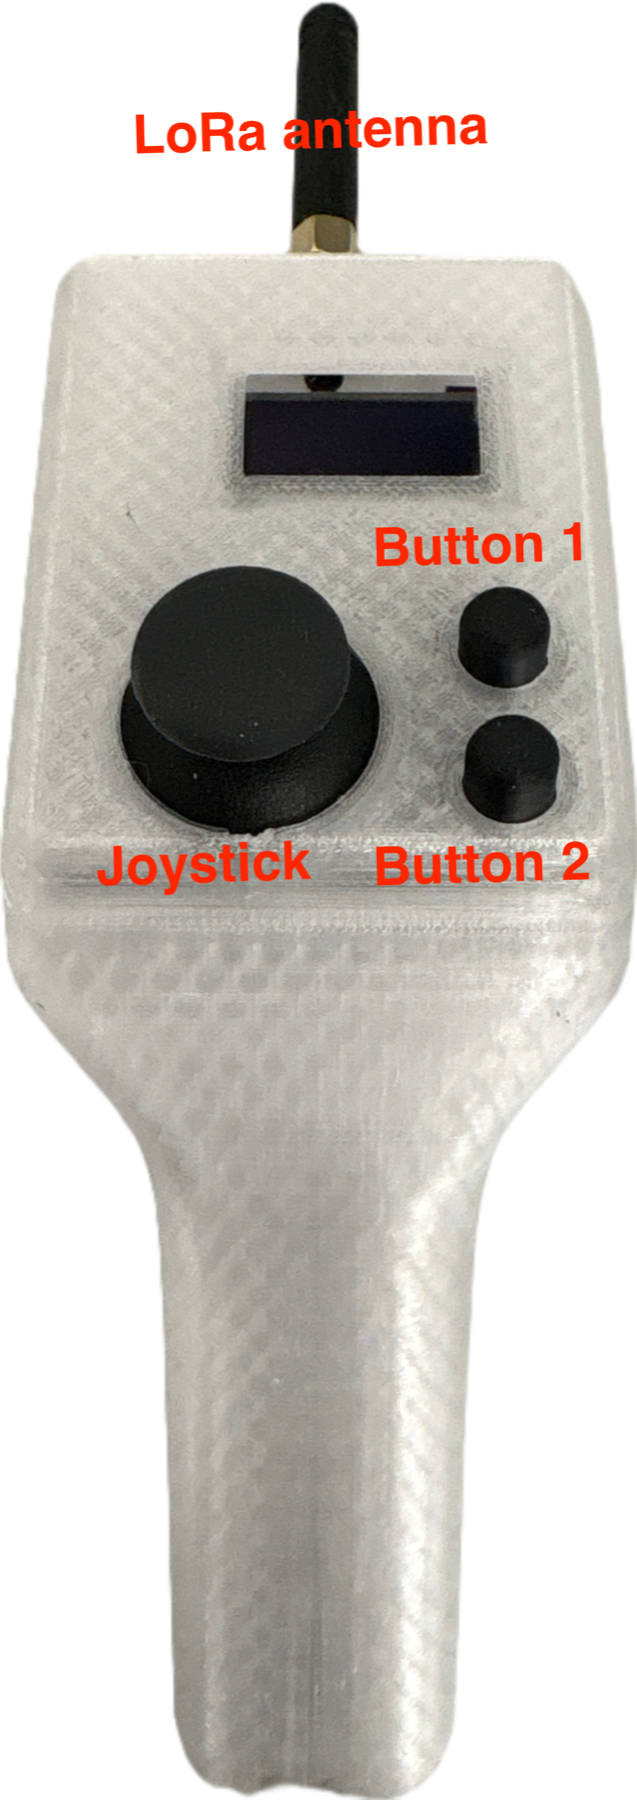
\includegraphics[keepaspectratio,alt={RobotController handheld showing the LoRa antenna, joystick, Button 1, and Button 2}]{assets/robotcontroller-controls.png}}
\caption{RobotController physical controls: LoRa antenna, joystick,
Button 1, and Button 2.}
\end{figure}

\begin{figure}
\centering
\pandocbounded{
\includegraphics[keepaspectratio,alt={Labeled Single Joystick Remote Controller display, joystick, buttons, and antenna}]{assets/display-remotecontroller.pdf}}
\caption{Single Joystick Remote Controller connections and controls:
robot-communication LoRa antenna, joystick, Buttons 1--3, Select,
charging/power connection, and OLED.}
\end{figure}

\begin{manualwarning}

\textbf{Never power the controller without its LoRa antenna.}
Hand-tighten the correct robot-communication LoRa antenna before
switching on.

\end{manualwarning}

\begin{figure}
\centering
\pandocbounded{
\includegraphics[keepaspectratio,alt={Eight numbered Single Joystick Remote Controller operation pictures}]{assets/remotecontroller-operation-guide.pdf}}
\caption{Each picture number matches the instruction below.}
\end{figure}

\begin{enumerate}
\tightlist
\item
  \textbf{Inspect and connect.} Check the case, joystick, buttons,
  battery, and antenna socket. Fit the LoRa antenna and let the joystick
  rest in the center.
\item
  \textbf{Power on.} Keep the robot restrained. Switch on the handheld.
  Confirm the OLED says \textbf{Hold}; Robot Lost is normal until the
  robot starts.
\item
  \textbf{Wait for the robot.} Switch on the robot. Do not continue
  until the OLED says Robot OK, RSSI is visible, and telemetry changes.
\item
  \textbf{Select Manual.} Short-press Button 1. Confirm the display
  changes to Manual. A button press is only a request; the displayed
  robot mode is the confirmation.
\item
  \textbf{Test direction.} Move the joystick slightly forward, reverse,
  left, and right. Stop immediately if the robot moves in the wrong
  direction.
\item
  \textbf{Stop.} Release the joystick and short-press Button 1 for Hold.
  Confirm CMD is zero and wheels stop.
\item
  \textbf{Use setup webpage when required.} Join
  \texttt{mars\_rc\_XXXXXX}, enter \texttt{alphaagtech}, and open
  \texttt{192.168.10.1}. Change speed/radio settings only while the
  robot is in Hold.
\item
  \textbf{Emergency.} Release the joystick and use the robot's physical
  emergency stop. Do not approach until the robot is confirmed
  stationary.
\end{enumerate}

\subsection{Buttons and screens}\label{buttons-and-screens}

{\def\LTcaptype{none} % do not increment counter
\begin{longtable}[]{@{}
  >{\raggedright\arraybackslash}p{(\linewidth - 2\tabcolsep) * \real{0.5000}}
  >{\raggedright\arraybackslash}p{(\linewidth - 2\tabcolsep) * \real{0.5000}}@{}}
\toprule\noalign{}
\begin{minipage}[b]{\linewidth}\raggedright
Control
\end{minipage} & \begin{minipage}[b]{\linewidth}\raggedright
Result
\end{minipage} \\
\midrule\noalign{}
\endhead
\bottomrule\noalign{}
\endlastfoot
Button 1 short & Manual/Hold; changing from Auto to Manual or Hold
automatically stops active autonomous navigation \\
Button 1 long & Sleep; Button 1 wakes \\
Button 2 short & Auto/Auto Pause; during an active mission, selecting
Auto Pause pauses autonomous navigation while retaining the mission for
Resume; also confirms calibration when prompted \\
Button 2 held & Enter Auto \\
Button 3 held & High speed while held \\
Joystick Select & Home -\textgreater{} Telemetry -\textgreater{}
Settings -\textgreater{} Calibration \\
\end{longtable}
}

\begin{figure}
\centering
\pandocbounded{
\includegraphics[keepaspectratio,alt={Single Joystick Remote Controller Home, Telemetry, Settings, and Calibration pages}]{assets/display-remotecontroller-pages.pdf}}
\caption{Home shows robot/mode/CMD/ACT; Telemetry shows GPS and age;
Settings changes radio/speed; Calibration shows joystick progress.}
\end{figure}

\subsection{Joystick calibration}\label{joystick-calibration}

\begin{enumerate}
\tightlist
\item
  Restrain the robot and open Calibration with Select; Hold is forced.
\item
  Let the stick center and short-press Button 2.
\item
  Move slowly to every endpoint and circle the outside edge several
  times.
\item
  Release to natural center and press Button 2 again.
\item
  Do not touch the stick during center sampling. Wait for Success and
  verify zero CMD at center.
\end{enumerate}

\subsection{Wi-Fi settings}\label{wi-fi-settings}

\begin{enumerate}
\tightlist
\item
  Join the Single Joystick Remote Controller network and remain
  connected when the phone reports No Internet.
\item
  Open the local address. Review battery, GPS, RSSI, and telemetry age.
\item
  Set slow/high speed values, save, reload, and test while restrained.
\item
  Record old LoRa values before changing them. Set the robot to the
  identical frequency, bandwidth, and SF.
\end{enumerate}

\protect\phantomsection\label{custom-operation}
\section{Dual Joystick Remote Controller operation
manual}\label{dual-joystick-remote-controller-operation-manual}

\begin{figure}
\centering
\pandocbounded{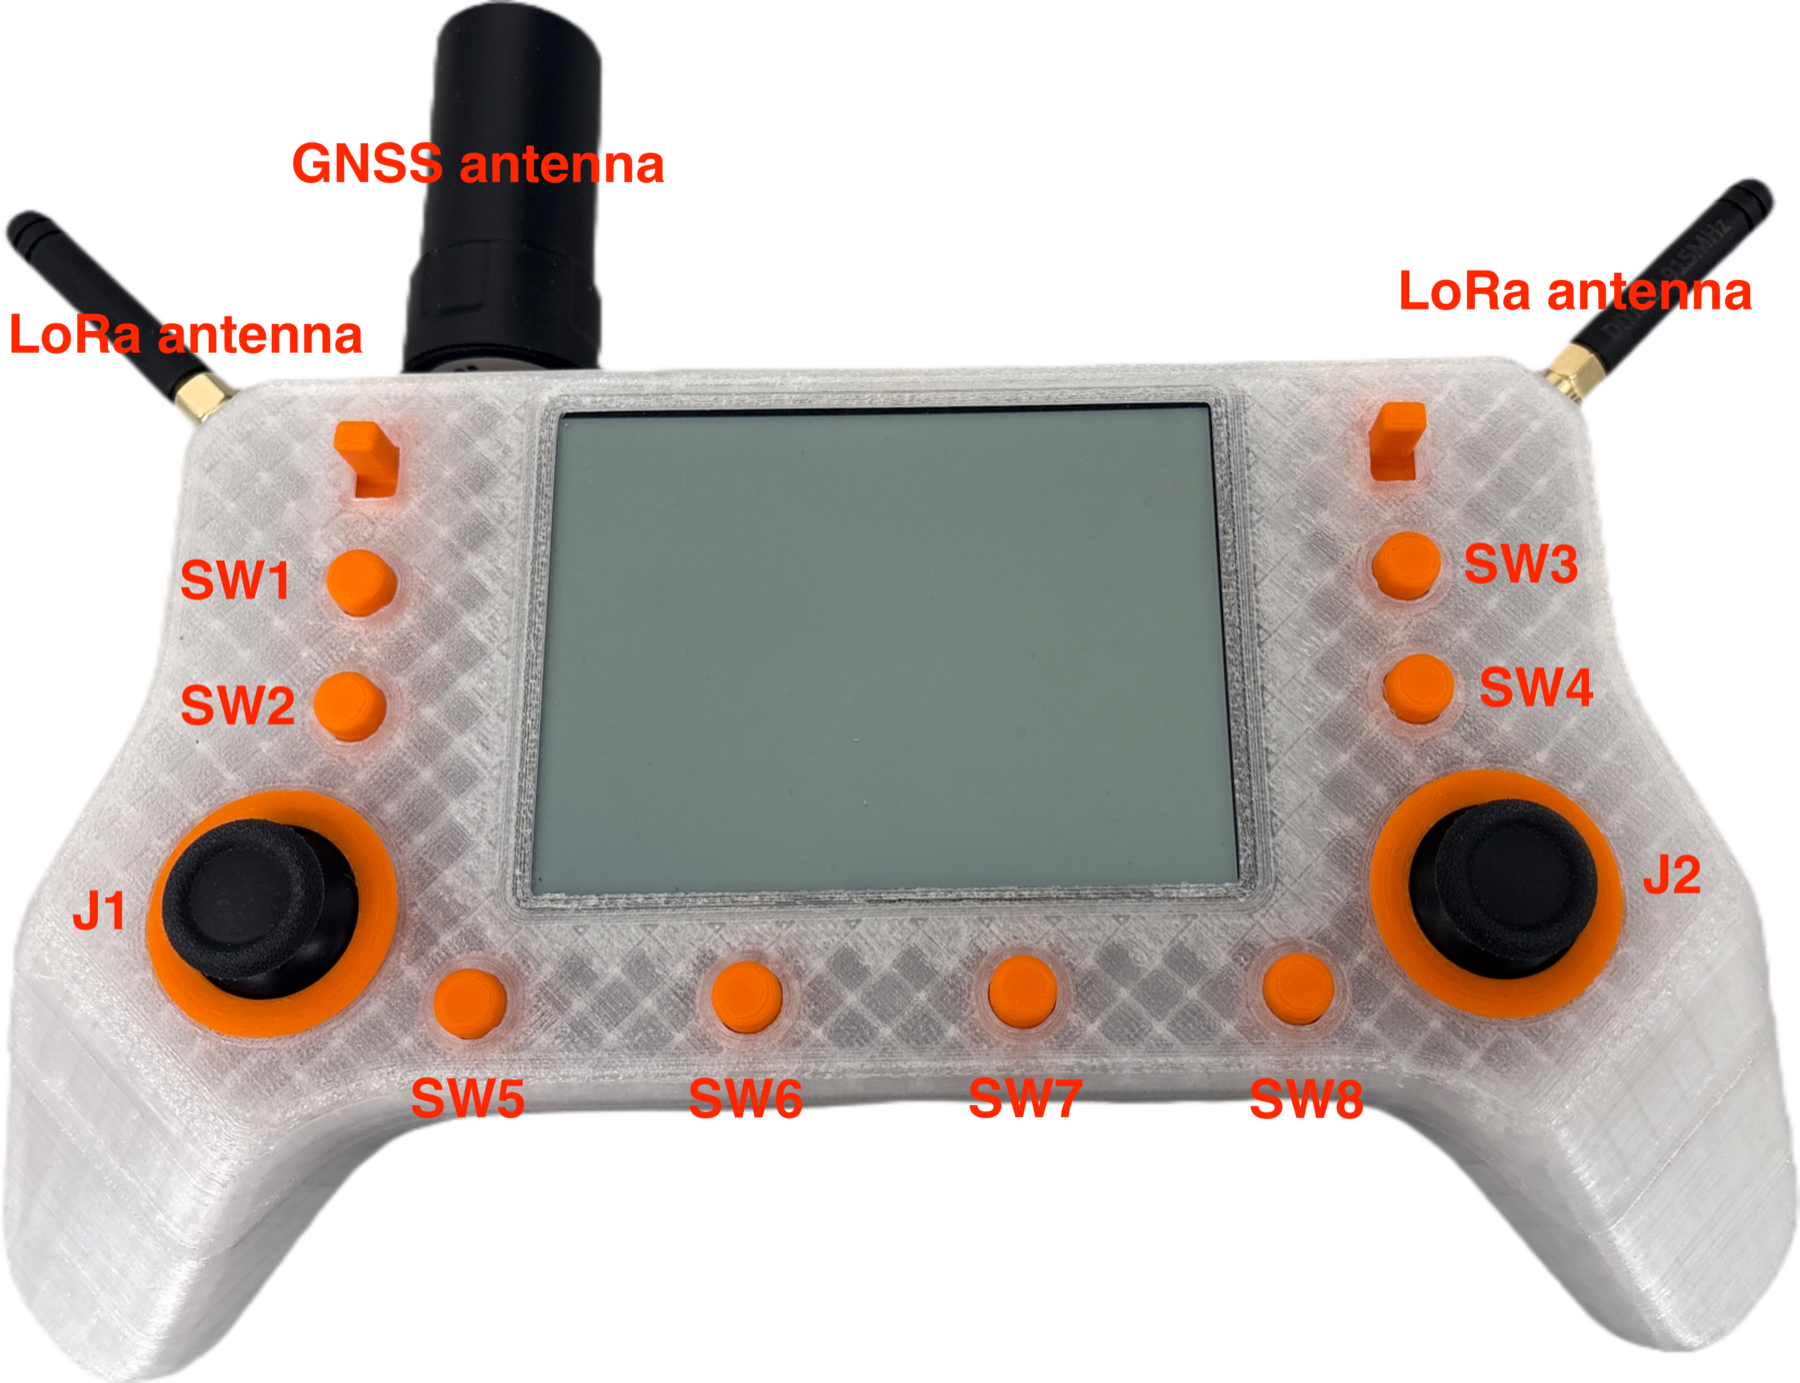
\includegraphics[keepaspectratio,alt={Custom RC Controller showing the left and right joysticks, Buttons 1 through 8, GNSS antenna, and two LoRa antennas}]{assets/custom-rc-controller-controls.png}}
\caption{Custom RC Controller physical controls: left and right
joysticks, Buttons 1--8, center GNSS antenna, and left/right LoRa
antennas. Facing the controller, the left antenna is RTK LoRa, the
middle antenna is GNSS, and the right antenna is robot-communication
LoRa.}
\end{figure}

\begin{manualwarning}

\textbf{Attach all three correct antennas before power-on.} Do not swap
the RTK LoRa, GNSS, and robot-communication LoRa antennas.

\end{manualwarning}

\begin{manualdanger}

\textbf{Keep RC LoRa and RTK LoRa on different radio settings.} The RTK
radio must match the RTK base, while the RC radio must match the robot.
Use the approved channel plan and verify both links independently.

\end{manualdanger}

\begin{figure}
\centering
\pandocbounded{
\includegraphics[keepaspectratio,alt={Six numbered Dual Joystick Remote Controller operation pictures}]{assets/custom-controller-operation-guide.pdf}}
\caption{Each picture number matches the instruction below.}
\end{figure}

\begin{enumerate}
\tightlist
\item
  \textbf{Prepare.} Inspect the unit. Facing the controller, fit the RTK
  LoRa antenna on the left, GNSS antenna in the middle, and
  robot-communication LoRa antenna on the right. Center J1/J2 and make
  sure no switch is held.
\item
  \textbf{Read Home.} Power on and verify Hold, zero CMD, UVC Disarmed,
  controller battery, robot Online, and fresh RSSI/telemetry.
\item
  \textbf{Drive.} Press SW5 for Manual and use J2 by default. Test at
  low speed; SW9 gives high speed only while held.
\item
  \textbf{Use pages.} SW1/SW2 move through pages or menu items, SW3
  selects/saves, and SW4 goes back/cancels.
\item
  \textbf{UVC warning.} After arming, an On request opens the warning.
  Check the secured area; SW3 confirms, SW4 cancels, and 10 seconds
  without action cancels.
\item
  \textbf{Use Wi-Fi.} Join \texttt{RC-Controller} with
  \texttt{alphaagtech}, open \texttt{192.168.4.1}, and configure the RC
  and RTK radios separately. Never copy the RC settings into the RTK
  radio; each radio matches its own endpoint and the two links must use
  non-overlapping field-approved settings.
\end{enumerate}

\begin{figure}
\centering
\pandocbounded{
\includegraphics[keepaspectratio,alt={All Dual Joystick Remote Controller display pages}]{assets/display-custom-controller-pages.pdf}}
\caption{Home, Robot Detail, GPS Detail, Settings, Joystick Calibration,
Joystick Mapping, Button Mapping, LoRa Settings, and Voice Volume.}
\end{figure}

\subsection{Calibration and mapping}\label{calibration-and-mapping}

\begin{enumerate}
\tightlist
\item
  Restrain the robot and open Settings -\textgreater{} Joystick
  Calibration.
\item
  Move J1/J2 through every endpoint while watching all four displayed
  axes.
\item
  Release both sticks; SW3 saves or SW4 cancels.
\item
  In Joystick Mapping choose J1 or J2 for driving, reverse axes if
  necessary, and use the smallest trim/deadband that produces stable
  zero.
\item
  In Button Mapping assign SW5--SW10. Each function may be used once;
  SW1--SW4 are fixed.
\end{enumerate}

\subsection{Radio, clock, voice, and firmware
webpage}\label{radio-clock-voice-and-firmware-webpage}

\begin{itemize}
\tightlist
\item
  \textbf{RC radio:} must match the robot's communication radio.
\item
  \textbf{RTK radio:} must match the RTK correction base and must not
  use the same channel/settings as RC. Separate the links according to
  the approved radio plan to prevent LoRa interference.
\item
  \textbf{Applied:} saved radio settings are active. Pending means wait.
  Failed means restore known-good values.
\item
  \textbf{Clock:} verify the phone time zone, then Sync Browser Time.
\item
  \textbf{Voice:} 0\% mutes alerts; higher values change in 10\% steps.
\item
  \textbf{Firmware:} select only the custom ESP32-S3 application image.
  Username is \texttt{admin}; password is \texttt{rccontroller}. Verify
  all functions after reboot.
\end{itemize}

\protect\phantomsection\label{controller-trouble}
\section{Controller troubleshooting}\label{controller-troubleshooting}

{\def\LTcaptype{none} % do not increment counter
\begin{longtable}[]{@{}
  >{\raggedright\arraybackslash}p{(\linewidth - 4\tabcolsep) * \real{0.3333}}
  >{\raggedright\arraybackslash}p{(\linewidth - 4\tabcolsep) * \real{0.3333}}
  >{\raggedright\arraybackslash}p{(\linewidth - 4\tabcolsep) * \real{0.3333}}@{}}
\toprule\noalign{}
\begin{minipage}[b]{\linewidth}\raggedright
Problem
\end{minipage} & \begin{minipage}[b]{\linewidth}\raggedright
What it means
\end{minipage} & \begin{minipage}[b]{\linewidth}\raggedright
What to do
\end{minipage} \\
\midrule\noalign{}
\endhead
\bottomrule\noalign{}
\endlastfoot
Robot Lost / Offline & No valid MAVLink reply from robot system ID 1 for
approximately one second. & Select Hold; verify robot power and
antennas; move closer; match RC LoRa settings; then inspect MAVLink
version, source ID and parse/CRC errors. \\
Good RSSI but no valid telemetry & RF packets are present but MAVLink
frames have the wrong version/ID, fail parsing, or contain unsupported
messages. & Keep Hold. Confirm MAVLink 2, controller system 255, robot
system 1, component IDs, one frame per packet and matching firmware. \\
Mode request repeats & No accepted \texttt{COMMAND\_ACK} or matching
robot heartbeat has completed the request. & Read the ACK result; verify
\texttt{MAV\_CMD\_DO\_SET\_MODE}, target component and custom-mode
value; correct the rejection before retrying. \\
Dual Joystick Remote Controller GPS is not sent & The onboard GPS fix is
invalid or older than 1.5 seconds. & Improve sky view/corrections and
verify fresh GPS status; stale fixes are intentionally not
transmitted. \\
Robot creeps at center & Joystick zero is incorrect. & Check free return
to center; recalibrate; increase deadband slightly; use only small
trim. \\
Direction is reversed & Axis mapping or wiring does not agree. & Stop;
select Hold; correct Dual Joystick Remote Controller axis reversal or
service Single Joystick Remote Controller/robot mapping; retest
restrained. \\
Webpage will not open & Phone left the local network or hostname failed.
& Stay connected despite No Internet; disable mobile-data switching/VPN;
use the numeric address. \\
Dual Joystick Remote Controller UVC On ignored & Not armed, warning
canceled/timed out, or no robot acknowledgment. & Verify UVC Armed,
robot link, relay status, then repeat deliberate confirmation. \\
Emergency overlay remains & Last robot heartbeat reported emergency. &
Make the robot safe and reset the physical system; wait for a new
non-emergency heartbeat. \\
\end{longtable}
}

\chapter{Component · Mobile robot and UVC
system}\label{component-mobile-robot-and-uvc-system}

\protect\phantomsection\label{robot}
\section{Mobile robot and UVC: component
overview}\label{mobile-robot-and-uvc-component-overview}

The robot uses two driven wheels and two steering axes. Robot master
node \texttt{0x0B} and slave node \texttt{0x0A} coordinate motor nodes 1
and 2 for steering and motor nodes 3 and 4 for driving. The installed
power hub connects the two robot sides and provides the CAN-controlled
status LED at node \texttt{0x0E}. The master receives handheld or
navigation commands, reads system status/GPS, and controls relay node
\texttt{0x0F}. The UVC system has four Philips lamps on left and right
physical AC power branches.

\subsection{Features}\label{features-1}

\begin{itemize}
\tightlist
\item
  2WD propulsion and 2WS steering.
\item
  Four installed CANopen motor nodes: steering 1--2 and drive 3--4.
\item
  Automatic precharge, motor-contactor control, steering homing and
  startup fault detection.
\item
  Power hub joining the two robot sides, with RGBA LED indications for
  startup, idle, running, link loss and safety states.
\item
  Hold, Manual, Auto, and Auto Pause modes.
\item
  LoRa handheld control and telemetry.
\item
  500 kbit/s CAN connection to motor controllers, robot master/slave,
  GPS rover, navigation interface, power hub, and UVC relay.
\item
  Robot Wi-Fi dashboard and configuration webpage.
\item
  Four external ports on each robot side: two contactor-switched
  battery-power ports and two CAN-bus ports.
\item
  Battery-powered PoE switch supplying the navigation controller
  network/power path.
\item
  Four robot-mounted UVC lamps: left side, right side, top-left, and
  top-right.
\item
  Routine UVC control commands all six relay channels together, with
  Arm, All Off, Disarm, heartbeat fail-safe, and CAN emergency shutdown.
\end{itemize}

\protect\phantomsection\label{robot-specs}
\section{Robot and UVC
specifications}\label{robot-and-uvc-specifications}

\subsection{Installed component list}\label{installed-component-list}

{\def\LTcaptype{none} % do not increment counter
\begin{longtable}[]{@{}
  >{\raggedright\arraybackslash}p{(\linewidth - 4\tabcolsep) * \real{0.3333}}
  >{\raggedright\arraybackslash}p{(\linewidth - 4\tabcolsep) * \real{0.3333}}
  >{\raggedright\arraybackslash}p{(\linewidth - 4\tabcolsep) * \real{0.3333}}@{}}
\toprule\noalign{}
\begin{minipage}[b]{\linewidth}\raggedright
Component
\end{minipage} & \begin{minipage}[b]{\linewidth}\raggedright
Installed model or rating
\end{minipage} & \begin{minipage}[b]{\linewidth}\raggedright
Manufacturer / notes
\end{minipage} \\
\midrule\noalign{}
\endhead
\bottomrule\noalign{}
\endlastfoot
Motor & \texttt{ELVM80100V48FH-M17-HD} & Leadshine \\
Motor driver & \texttt{ELD2-CAN7030B} & Leadshine \\
Steering-wheel gearbox & \texttt{FAD-110D-50-P2-19-70-90-M6-42} & OC
Drive Machinery Co. \\
Drive-wheel gearbox & \texttt{FAD-110D-70-P2-19-70-90-M6-42} & OC Drive
Machinery Co. \\
Battery pack & 48 V, 80 Ah & Two packs installed, one on each robot
side \\
Inverter & Victron Inverter 48/375 VE & Victron; two installed, one per
robot side \\
UVC ballast & \texttt{KTEB-254HO-UV-PS} & One ballast per installed UVC
bulb \\
UVC bulb & \texttt{TUV\ PL-L\ 55W/4P/HF} & Philips; four installed \\
\end{longtable}
}

\subsection{System specifications}\label{system-specifications}

{\def\LTcaptype{none} % do not increment counter
\begin{longtable}[]{@{}
  >{\raggedright\arraybackslash}p{(\linewidth - 2\tabcolsep) * \real{0.5000}}
  >{\raggedright\arraybackslash}p{(\linewidth - 2\tabcolsep) * \real{0.5000}}@{}}
\toprule\noalign{}
\begin{minipage}[b]{\linewidth}\raggedright
Item
\end{minipage} & \begin{minipage}[b]{\linewidth}\raggedright
Specification
\end{minipage} \\
\midrule\noalign{}
\endhead
\bottomrule\noalign{}
\endlastfoot
Controller firmware & \texttt{1.0.1} \\
Motion & Two drive axes and two steering axes \\
Motor nodes & 1--2 steering; 3--4 drive \\
CAN bus & 500 kbit/s \\
Startup timing & Approximately 4 s precharge, main-contactor closure,
0.5 s precharge overlap, then 5 s safety wait before CAN/node checks \\
Power hub & Cross-chassis connection between robot sides; CAN node 14
(\texttt{0x0E}); RGBA status LED \\
Robot Wi-Fi & \texttt{mars\_h\_XXXXXX}; local dashboard \\
Relay & CAN node decimal 15 (\texttt{0x0F}); electronics powered by 5 V
from a power-hub 5 V CAN port; 500 kbit/s CANH/CANL \\
Relay groups & Group A: left-side + top-left; Group B: right-side +
top-right; all six channels are commanded together by robot firmware \\
Relay Wi-Fi & \texttt{can\_relay\_XXXXXX}; \texttt{192.168.10.1} \\
Fail-safe & All six channels Off/Disarm on CAN emergency or missing
robot-master heartbeat \\
Heartbeat timeout & Approximately 3 seconds at relay \\
\end{longtable}
}

\protect\phantomsection\label{robot-connections}
\section{Robot connections and side
ports}\label{robot-connections-and-side-ports}

\begin{figure}
\centering
\pandocbounded{
\includegraphics[keepaspectratio,alt={Left and right robot sides each showing two battery-power ports and two four-wire CAN-bus ports, plus the battery-powered PoE switch}]{assets/robot-side-ports.pdf}}
\caption{Each robot side has four ports: two battery-power ports
switched by the main contactor and two CAN-bus ports carrying 12 V, GND,
CANH, and CANL. The installed power hub connects the left and right
sides and carries the system status LED.}
\end{figure}

\begin{manualwarning}

\textbf{Main contactor:} the two power ports on each side are connected
to robot battery power through the electrically controlled contactor.
They can become energized when the contactor closes. Do not assume a
connector is safe because the robot is in Hold.

\end{manualwarning}

{\def\LTcaptype{none} % do not increment counter
\begin{longtable}[]{@{}
  >{\raggedright\arraybackslash}p{(\linewidth - 4\tabcolsep) * \real{0.3333}}
  >{\raggedright\arraybackslash}p{(\linewidth - 4\tabcolsep) * \real{0.3333}}
  >{\raggedright\arraybackslash}p{(\linewidth - 4\tabcolsep) * \real{0.3333}}@{}}
\toprule\noalign{}
\begin{minipage}[b]{\linewidth}\raggedright
Connection
\end{minipage} & \begin{minipage}[b]{\linewidth}\raggedright
Purpose
\end{minipage} & \begin{minipage}[b]{\linewidth}\raggedright
Operator/engineer check
\end{minipage} \\
\midrule\noalign{}
\endhead
\bottomrule\noalign{}
\endlastfoot
RC LoRa antenna & Handheld commands and telemetry & Tight, undamaged, RC
settings match only the controller \\
Battery power ports---2 per side & Contactor-switched robot battery
supply for approved loads & Correct voltage/polarity, connector label,
fuse/protection, contactor Off before mating \\
CAN-bus ports---2 per side & Combined auxiliary power and CAN
communications & Pinout is 12 V, GND, CANH, CANL; never confuse with
battery-power port \\
Power hub + LED, node 14 & Cross-chassis connection joining the two
robot sides and displaying system status & Hub secure; inter-side
connections tight; LED visible; CAN heartbeat and SDO response
present \\
PoE switch & Network connection and PoE supply for the navigation
controller & Powered from robot battery power through the installed
protected supply path; link and PoE indicators normal \\
Drive motors, nodes 3--4 & Forward and reverse & Correct direction and
feedback \\
Steering motors, nodes 1--2 & Wheel angle & Homed, no fault, correct
actual angle \\
Relay Group A & Left-side and top-left lamps & Two correct physical
labels and matching applied feedback \\
Relay Group B & Right-side and top-right lamps & Two correct physical
labels and matching applied feedback \\
Emergency stop & Independent safe stop & Accessible and tested before
operation \\
\end{longtable}
}

\subsection{Side-port connection
procedure}\label{side-port-connection-procedure}

\begin{enumerate}
\tightlist
\item
  Select Hold, switch UVC Off/Disarm, open the main contactor, and
  follow the site lockout procedure.
\item
  Read the port label. Identify \textbf{BATTERY POWER} or \textbf{CAN
  BUS}; do not choose by connector appearance alone.
\item
  Inspect pins, seals, keying, strain relief, cable rating, and damage.
  Do not connect a wet, bent, or unlabeled plug.
\item
  For a CAN port, verify the cable pinout end-to-end: 12 V, GND, CANH,
  CANL. Check bus termination and avoid adding an unintended terminator.
\item
  For a battery port, verify the approved load, operating voltage,
  polarity, branch protection, and current rating before mating.
\item
  Mate without forcing, secure the connector, route the cable away from
  steering/wheels/UVC fixtures, then restore power.
\item
  Confirm the intended device only: supply voltage, CAN online state, or
  PoE/link indication. Stop and isolate immediately for heat, odor,
  arcing, wrong voltage, or CAN faults.
\end{enumerate}

\protect\phantomsection\label{robot-battery}
\section{Battery compartments and
charging}\label{battery-compartments-and-charging}

The robot has \textbf{two separate battery packs}: one in the locked
compartment on the left side and one in the locked compartment on the
right side. Open one compartment, support and move its battery out far
enough to reach the battery charge port, charge it with the approved
charger, then return and secure it before repeating the procedure on the
other side.

\begin{figure}
\centering
\pandocbounded{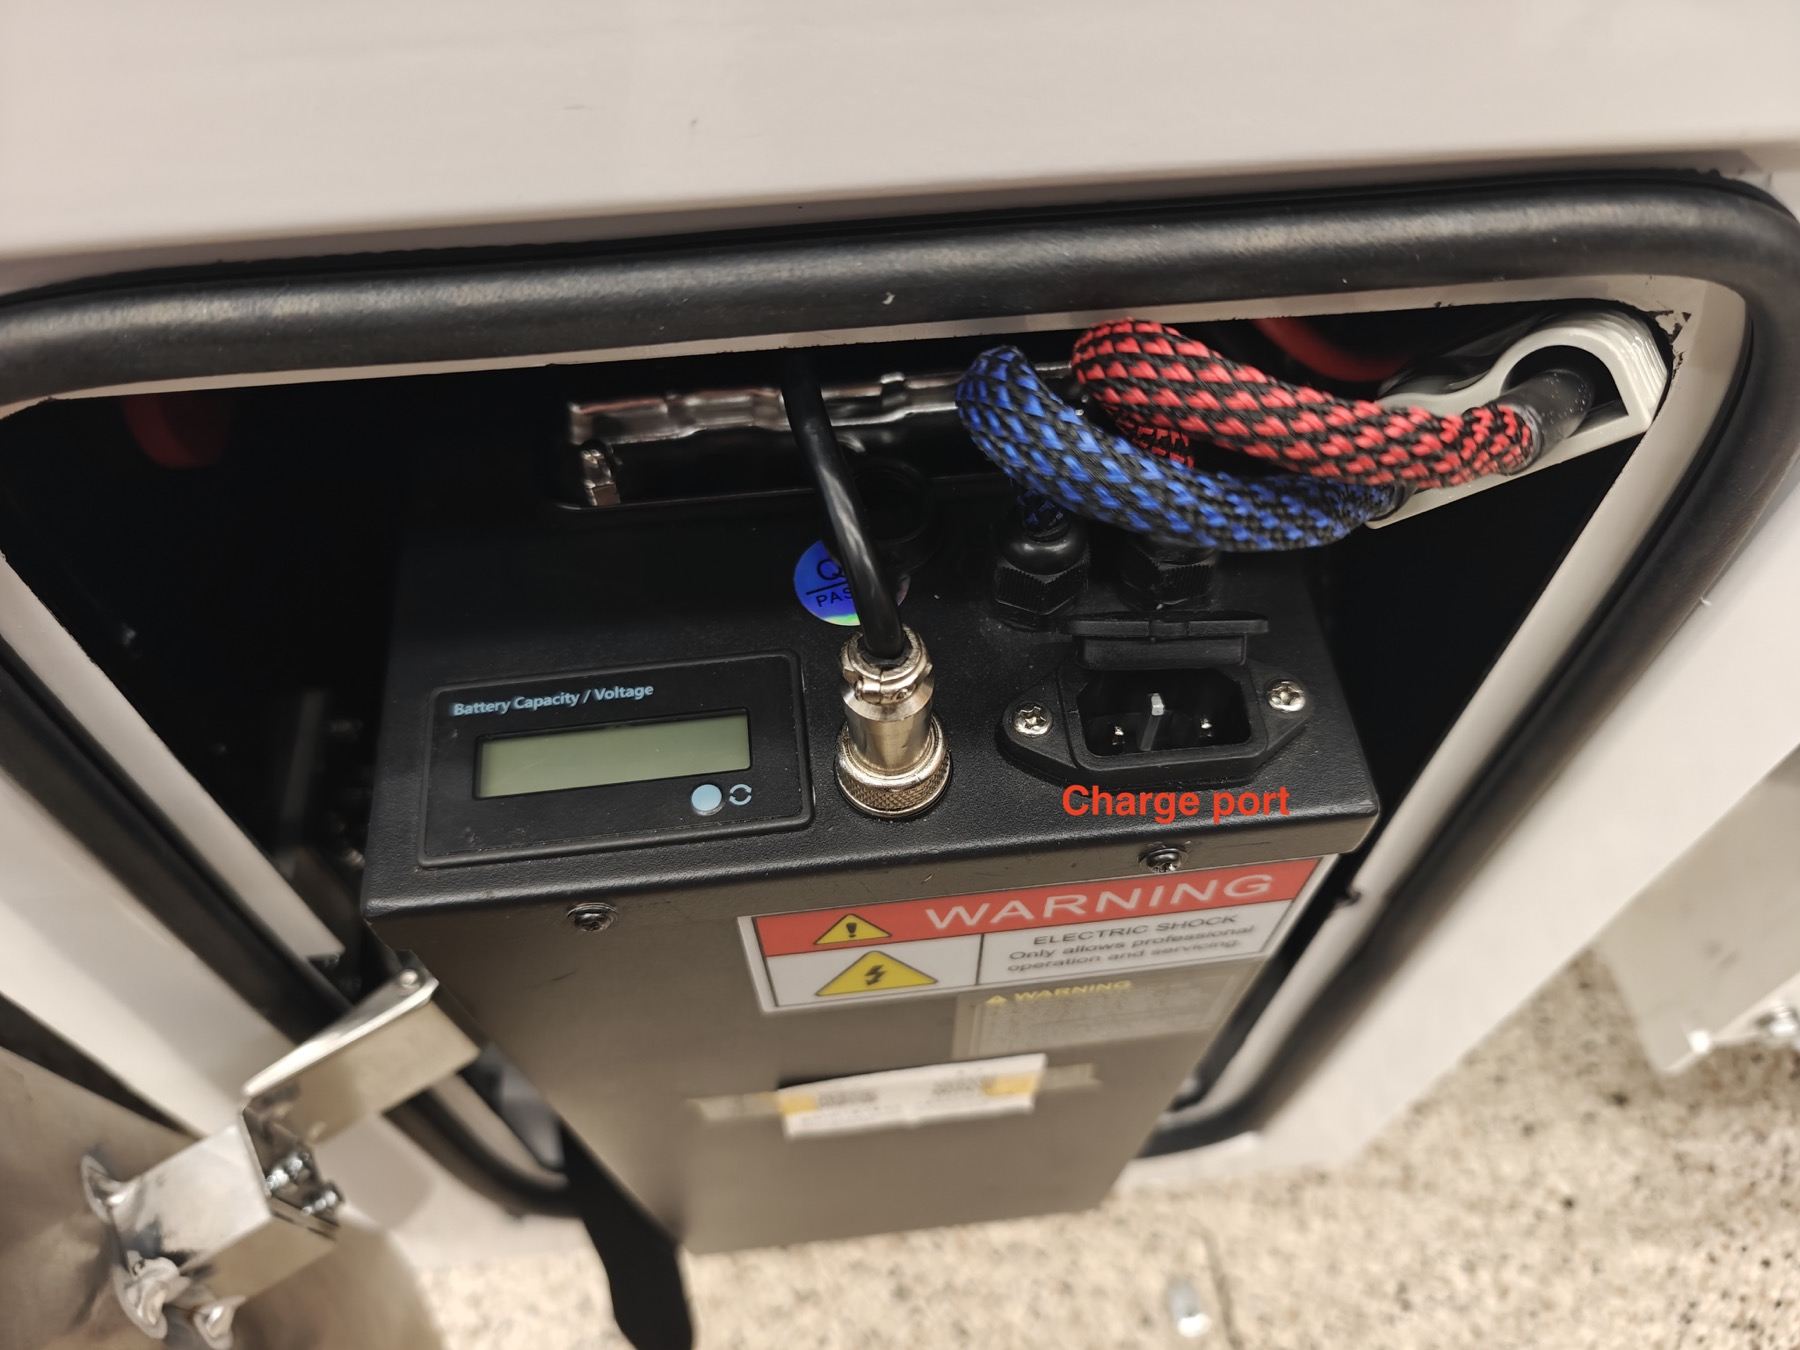
\includegraphics[keepaspectratio,alt={Robot battery moved out of its compartment with its battery charge port labeled}]{assets/robot-battery-charge-port.jpg}}
\caption{The charge port is on the battery itself. Its connector shape
does not make it an AC mains inlet.}
\end{figure}

\begin{figure}
\centering
\pandocbounded{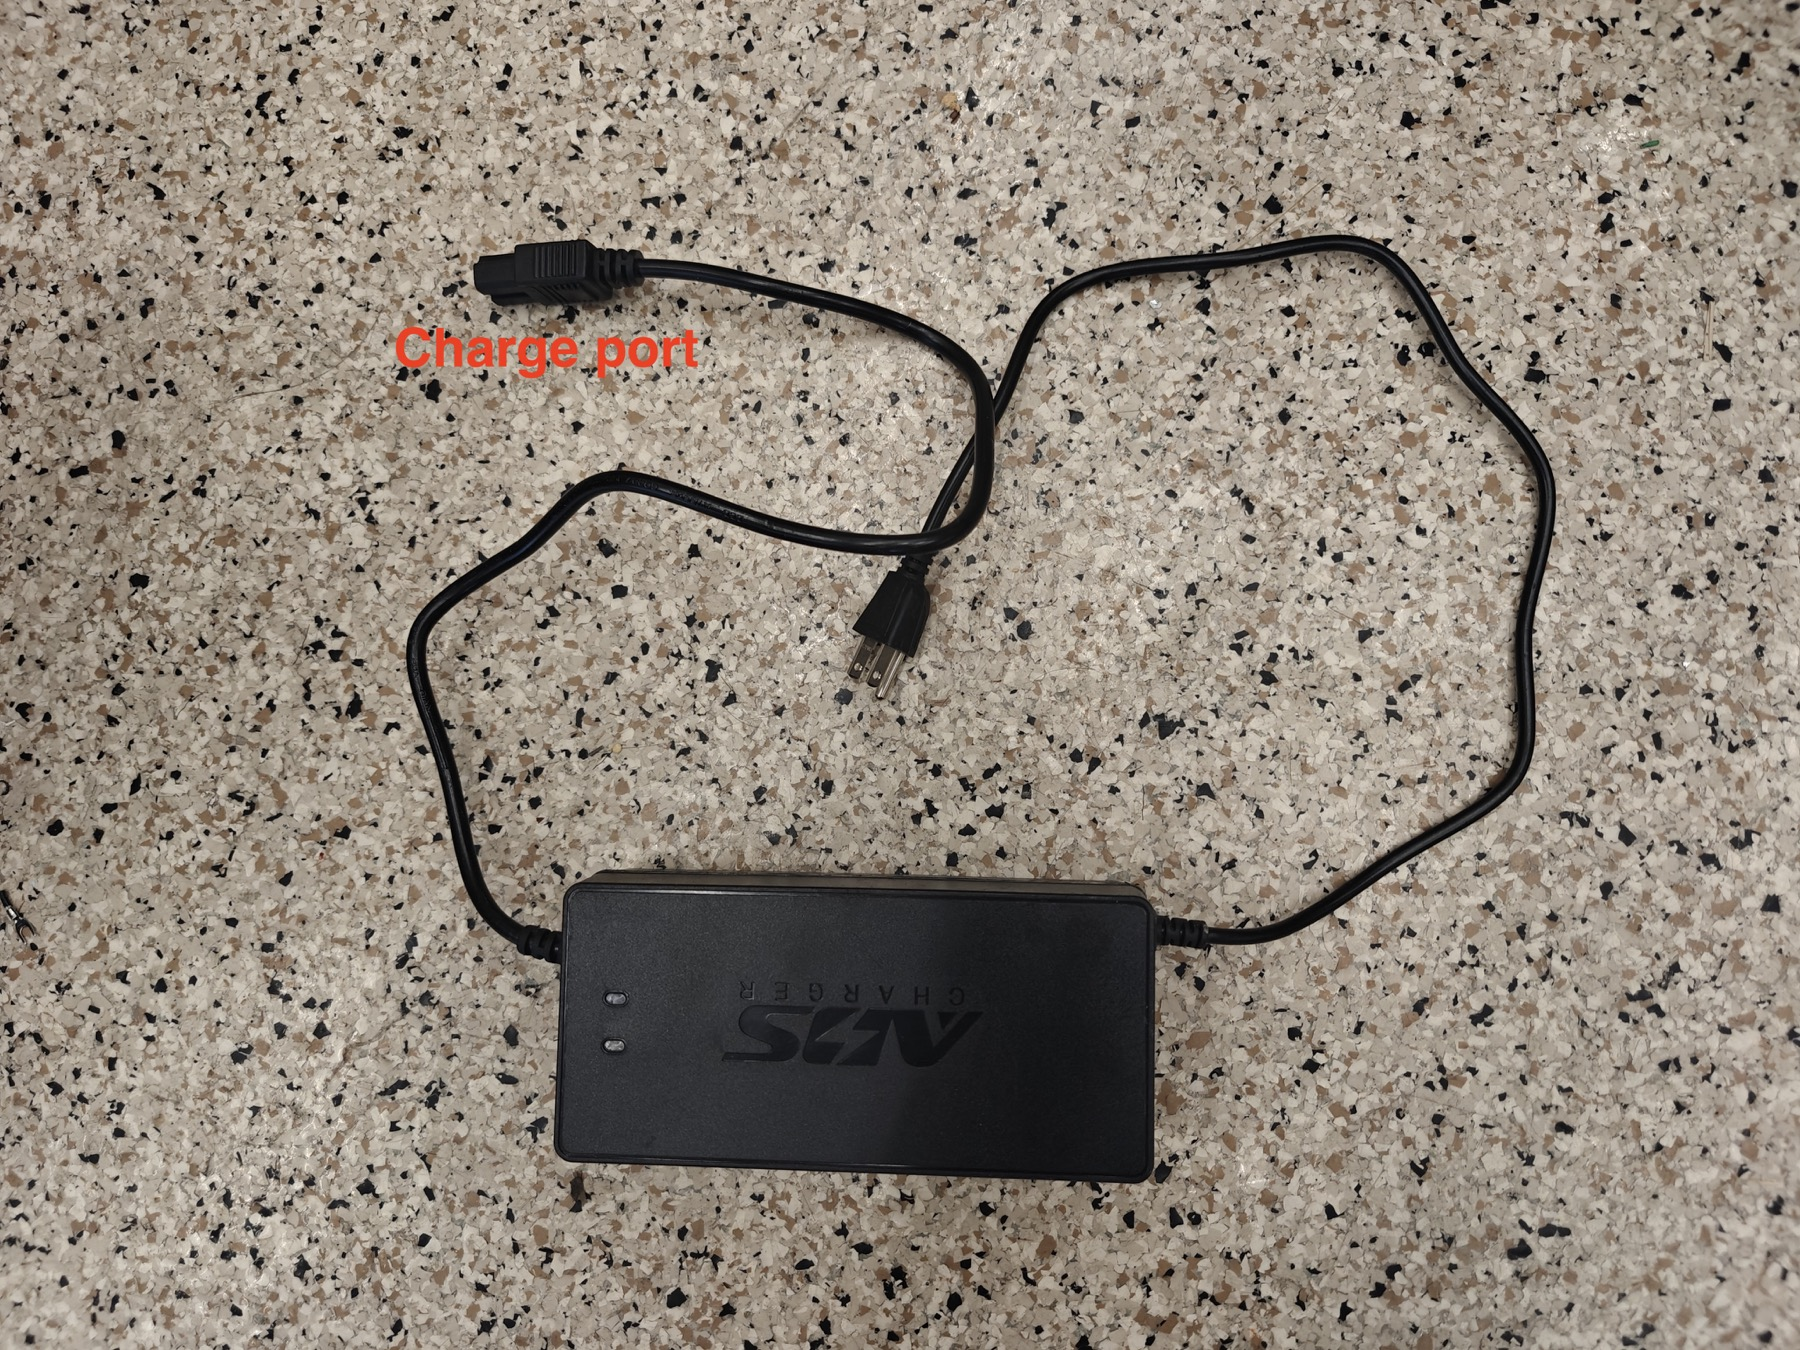
\includegraphics[keepaspectratio,alt={Approved robot battery charger showing its AC input plug and battery-output connector}]{assets/robot-battery-charger.jpg}}
\caption{The charger has two different connections: its AC input plug
connects to the correctly rated wall outlet, while its battery-output
connector connects to the battery charge port.}
\end{figure}

\begin{manualdanger}

\textbf{THE BATTERY CHARGE PORT IS NOT AN AC PORT.} Never connect
wall-outlet/mains AC, an AC power cord, or any other direct AC source to
the battery charge port---even if a connector appears to fit. Only the
battery-output connector from the charger approved for this battery may
connect to that port. Connect the charger's AC input only to a correctly
rated wall outlet and follow the charger label.

\end{manualdanger}

\begin{manualdanger}

\textbf{Battery charging can involve hazardous voltage, high fault
current, heat and fire risk.} Never charge a wet, damaged, swollen,
leaking, unusually hot, or unlabeled battery. Keep ignition sources away
and follow the battery, charger, and site emergency instructions.

\end{manualdanger}

\subsection{Prepare the robot and
battery}\label{prepare-the-robot-and-battery}

\begin{enumerate}
\tightlist
\item
  Park the robot on stable, dry ground in the designated charging area
  with ventilation and unobstructed emergency access.
\item
  Stop any mission, center the joystick, select Hold, and verify zero
  motion. Command UVC All Off, verify all four lamps Off, Disarm, and
  open the physical UVC disconnect.
\item
  Switch the robot off using the approved shutdown procedure. Do not
  begin while the contactor is closed or the robot is capable of motion.
\item
  Identify the battery side to charge. Confirm the compartment key and
  the charger approved for that exact battery pack. Charge one battery
  at a time unless the approved equipment and site procedure explicitly
  allow otherwise.
\item
  Unlock and open the selected battery compartment. Support the cover,
  disconnect or release the battery only as specified by its manual, and
  carefully slide or lift the battery out far enough to access the
  charge port. Support its weight; do not pull on cables or allow the
  battery to fall.
\item
  Inspect the battery housing, display, cables, terminals, charge port,
  protective cover, QR label, and charger. Stop and tag the equipment
  for service if anything is loose, wet, contaminated, cracked,
  corroded, swollen, leaking, burnt, or unusually hot.
\end{enumerate}

\subsection{Connect and charge}\label{connect-and-charge}

\begin{enumerate}
\setcounter{enumi}{6}
\tightlist
\item
  Keep the charger disconnected from AC power while making the
  battery-side connection unless the charger's own instructions require
  a different sequence.
\item
  Identify the charger's \textbf{battery-output connector} and connect
  it to the battery charge port without forcing it. Do not connect the
  wall-outlet AC plug or any direct AC source to the battery.
\item
  Check that the connector is fully seated and the cable is protected
  from the compartment edge, wheels, steering, and foot traffic. Then
  connect the charger's AC input plug to a correctly rated wall outlet
  and energize it according to the charger instructions.
\item
  Confirm normal charging on the charger and battery indicators. Monitor
  the battery and charger for faults, unusual heat, odor, smoke, noise,
  swelling, leakage, or cable damage. Stop and follow the battery
  emergency procedure for any abnormal condition.
\end{enumerate}

\subsection{Finish and secure}\label{finish-and-secure}

\begin{enumerate}
\setcounter{enumi}{10}
\tightlist
\item
  When charging is complete, switch off or unplug the charger from AC
  power before disconnecting its battery-output connector, unless the
  charger manual specifies another order. Never pull on the cable.
\item
  Inspect the charge port and refit its protective cover. Carefully
  return the battery fully into its compartment, reconnect and secure it
  according to the battery manual, and confirm no cable is pinched or
  strained.
\item
  Close and lock the compartment. Verify it is latched, then repeat the
  complete procedure for the battery on the other side.
\item
  Before returning the robot to service, confirm both batteries are
  secured, both compartment locks are closed, no charger remains
  attached, both battery states are acceptable, and the robot passes the
  normal \hyperref[robot-startup]{power-on sequence}.
\end{enumerate}

\subsection{Battery Bluetooth app and
manual}\label{battery-bluetooth-app-and-manual}

Each battery has built-in Bluetooth communication. Scan the QR code
printed on that battery to obtain the manufacturer's app and battery
manual. Before installing, verify that the QR destination and app
publisher match the battery manufacturer. Follow the battery manual for
pairing, status interpretation, alarms, and maintenance. Bluetooth/app
readings supplement---but do not replace---the battery display, charger
indicators, physical inspection, or charging safety checks.

\subsection{Charging troubleshooting}\label{charging-troubleshooting}

{\def\LTcaptype{none} % do not increment counter
\begin{longtable}[]{@{}
  >{\raggedright\arraybackslash}p{(\linewidth - 2\tabcolsep) * \real{0.5000}}
  >{\raggedright\arraybackslash}p{(\linewidth - 2\tabcolsep) * \real{0.5000}}@{}}
\toprule\noalign{}
\begin{minipage}[b]{\linewidth}\raggedright
Symptom
\end{minipage} & \begin{minipage}[b]{\linewidth}\raggedright
Action
\end{minipage} \\
\midrule\noalign{}
\endhead
\bottomrule\noalign{}
\endlastfoot
Charger does not start & De-energize it. Verify the approved charger,
correctly rated AC input, seated battery-output connector, battery
charge port, and charger indication. Never test the battery port with
direct AC. \\
Charger reports a fault & Stop charging, record the code/indicator,
isolate the charger, and follow the charger/battery manual. Do not
repeatedly reconnect to clear an unexplained fault. \\
Battery or connector becomes hot, smells, swells, leaks, or smokes & Use
the site battery emergency plan immediately. Do not touch, move, open,
or energize the robot unless the trained emergency procedure directs
it. \\
Battery will not slide out or return securely & Do not force it or
operate the robot. Inspect the retainers, cable routing, compartment,
battery alignment, and damage; obtain service assistance. \\
QR code or Bluetooth app does not work & Use the printed battery model
and manufacturer support information to obtain the official manual/app.
Do not install an app from an unverified publisher. \\
One side charges but the other does not & Treat each pack independently.
Verify the second battery's charger compatibility, charge port,
connector, battery condition, and fault status; do not infer its state
from the first battery. \\
\end{longtable}
}

\protect\phantomsection\label{power-hub}
\section{Power hub and status LED: component
manual}\label{power-hub-and-status-led-component-manual}

The power hub distributes regulated 12 V and 5 V power, provides
multiple CAN connection points, joins devices on the 500 kbit/s robot
CAN backbone, and controls the visible red/green/blue/white status LED.

\subsection{Features and
specifications}\label{features-and-specifications}

{\def\LTcaptype{none} % do not increment counter
\begin{longtable}[]{@{}
  >{\raggedright\arraybackslash}p{(\linewidth - 2\tabcolsep) * \real{0.5000}}
  >{\raggedright\arraybackslash}p{(\linewidth - 2\tabcolsep) * \real{0.5000}}@{}}
\toprule\noalign{}
\begin{minipage}[b]{\linewidth}\raggedright
Item
\end{minipage} & \begin{minipage}[b]{\linewidth}\raggedright
Installed specification
\end{minipage} \\
\midrule\noalign{}
\endhead
\bottomrule\noalign{}
\endlastfoot
Power distribution & Six 12 V CAN ports, four 5 V CAN ports, two 12 V
power-only ports and two 5 V power-only ports \\
CANopen node & 14 (\texttt{0x0E}) \\
CAN rate & 500 kbit/s \\
LED channels & Red, green, blue and dedicated white; commanded/applied
values 0--255 \\
PWM & 500 Hz, 9-bit timer; output limited to approximately 50\% maximum
PWM duty for fixture current/thermal control \\
Automatic control & Robot master writes mode object \texttt{0x2004} by
SDO, retries failures and reasserts the current mode at least every 2
seconds \\
Local emergency behavior & A nonzero CAN EMCY selects solid red
locally \\
Wi-Fi AP & \texttt{rgba\_led\_XXXXXX}; password \texttt{alphaagtech};
channel 1; maximum two clients \\
Web addresses & \texttt{http://rgba\_led.local} or
\texttt{http://192.168.10.1} \\
\end{longtable}
}

\subsection{Port, connector and pinout schedule}\label{power-hub-ports}

\begin{figure}
\centering
\pandocbounded{
\includegraphics[keepaspectratio,alt={Power hub 12 volt and 5 volt port map with GPS rover UVC relay and navigation connections}]{assets/power-hub-port-map.pdf}}
\caption{The GNSS rover and UVC relay receive 5 V operating power and
CAN from 5 V CAN ports. The navigation controller uses another 5 V
CAN-group connector for communication, while PoE supplies its operating
power.}
\end{figure}

{\def\LTcaptype{none} % do not increment counter
\begin{longtable}[]{@{}
  >{\raggedright\arraybackslash}p{(\linewidth - 6\tabcolsep) * \real{0.2500}}
  >{\raggedright\arraybackslash}p{(\linewidth - 6\tabcolsep) * \real{0.2500}}
  >{\raggedright\arraybackslash}p{(\linewidth - 6\tabcolsep) * \real{0.2500}}
  >{\raggedright\arraybackslash}p{(\linewidth - 6\tabcolsep) * \real{0.2500}}@{}}
\toprule\noalign{}
\begin{minipage}[b]{\linewidth}\raggedright
Function / board reference
\end{minipage} & \begin{minipage}[b]{\linewidth}\raggedright
Board connector
\end{minipage} & \begin{minipage}[b]{\linewidth}\raggedright
Cable-side mating housing
\end{minipage} & \begin{minipage}[b]{\linewidth}\raggedright
Pinout and use
\end{minipage} \\
\midrule\noalign{}
\endhead
\bottomrule\noalign{}
\endlastfoot
\begin{minipage}[t]{\linewidth}\raggedright
12 V CAN\\
\texttt{J1–J4}\strut
\end{minipage} & \begin{minipage}[t]{\linewidth}\raggedright
\href{https://www.molex.com/en-us/products/part-detail/469990014}{Molex
46999-0014}\\
Mini-Fit Jr., 4 circuits\strut
\end{minipage} & \begin{minipage}[t]{\linewidth}\raggedright
\href{https://www.molex.com/en-us/products/part-detail/39012040}{Molex
39-01-2040} (5557 series)\\
Female crimp terminals are selected separately for the installed wire
gauge/current.\strut
\end{minipage} & 1: 12 V; 2: CANH; 3: CANL; 4: GND. For approved 12 V
CAN devices. \\
\begin{minipage}[t]{\linewidth}\raggedright
12 V CAN\\
\texttt{J9–J10}\strut
\end{minipage} &
\href{https://www.amphenol-sine.com/ATP13-4P-BM03GRY-4-Position-90\%C2\%B0-PCB-Flange-Mount-Receptacle-Molded-Tin-Pins-Grey-Comparable-to-PN-DTP13-4P-E028_p_10053.html}{Amphenol
Sine ATP13-4P-BM03GRY} &
\href{https://www.amphenol-sine.com/ATP06-4S-4-Way-Plug-Female-Comparable-to-PN-DTP06-4S_p_916.html}{ATP06-4S}
plug, plus the specified wedge lock, seals and size-12 socket contacts &
1: 12 V; 2: CANH; 3: CANL; 4: GND. Sealed 12 V CAN connection. \\
\begin{minipage}[t]{\linewidth}\raggedright
5 V CAN\\
\texttt{J5–J8}\strut
\end{minipage} & \begin{minipage}[t]{\linewidth}\raggedright
\href{https://www.molex.com/en-us/products/part-detail/0430450402}{Molex
43045-0402}\\
Micro-Fit 3.0, 4 circuits\strut
\end{minipage} & \begin{minipage}[t]{\linewidth}\raggedright
\href{https://www.molex.com/en-us/products/part-detail/0430250400}{Molex
43025-0400}\\
Female terminals selected separately for wire gauge/current.\strut
\end{minipage} & 1: 5 V; 2: CANH; 3: CANL; 4: GND. The GNSS rover and
UVC relay receive 5 V operating power and CAN here. Navigation CAN also
uses this group, but navigation operating power comes from PoE. \\
\begin{minipage}[t]{\linewidth}\raggedright
12 V power only\\
\texttt{J12–J13}\strut
\end{minipage} & \begin{minipage}[t]{\linewidth}\raggedright
\href{https://www.molex.com/en-us/products/part-detail/768250002}{Molex
76825-0002}\\
Mega-Fit, 2 circuits\strut
\end{minipage} & \begin{minipage}[t]{\linewidth}\raggedright
\href{https://www.molex.com/en-us/products/part-detail/1716920102}{Molex
171692-0102}\\
Female terminals selected separately for wire gauge/current.\strut
\end{minipage} & 1: 12 V; 2: GND. Approved 12 V loads only; no CAN. \\
\begin{minipage}[t]{\linewidth}\raggedright
5 V power only\\
\texttt{J14–J15}\strut
\end{minipage} & \begin{minipage}[t]{\linewidth}\raggedright
Molex 43045-0200\\
Micro-Fit 3.0, 2 circuits\strut
\end{minipage} & \begin{minipage}[t]{\linewidth}\raggedright
\href{https://www.molex.com/en-us/products/part-detail/0430250200}{Molex
43025-0200}\\
Female terminals selected separately for wire gauge/current.\strut
\end{minipage} & 1: 5 V; 2: GND. Approved 5 V loads only; no CAN. \\
\begin{minipage}[t]{\linewidth}\raggedright
VIN input\\
\texttt{J16}\strut
\end{minipage} & 2-pin generic connector symbol; production part number
is not assigned in the board design & Match the connector fitted to the
serviced board; confirm against the production BOM before ordering & 1:
VIN; 2: VIN−. Qualified field service only. \\
\begin{minipage}[t]{\linewidth}\raggedright
Fused VIN outputs\\
\texttt{J11}, \texttt{J17}\strut
\end{minipage} & 2-pin generic connector symbol; production part number
is not assigned in the board design & Match the connector fitted to the
serviced board; confirm against the production BOM before ordering & 1:
fused VIN output; 2: VIN−. Qualified field service only. \\
\end{longtable}
}

Housing part numbers do not include crimp contacts, seals, secondary
locks or wire. Use the connector manufacturer\textquotesingle s
application specification and an approved crimp tool; choose contacts
for the actual conductor size, insulation diameter and circuit current.
Never substitute a housing solely because it appears to fit.

\begin{manualdanger}

\textbf{Wrong-voltage connection can destroy equipment.} Read the
printed voltage label before mating a connector. Never select a port by
connector shape alone, and never connect a 5 V device to a 12 V CAN or
power port.

\end{manualdanger}

\subsubsection{Installed device
assignments}\label{installed-device-assignments}

\begin{itemize}
\tightlist
\item
  \textbf{GNSS rover:} connect to a labelled 5 V CAN port. Pin 1
  supplies its 5 V operating power; pins 2/3 carry CANH/CANL and pin 4
  is GND. See \hyperref[gps-connections]{GPS connections}.
\item
  \textbf{UVC relay:} connect node 15 to its assigned 5 V CAN port. Pin
  1 supplies the relay electronics with 5 V; pins 2/3 carry CANH/CANL
  and pin 4 is GND. The relay contacts separately switch 120 VAC to the
  four ballast inputs. Never connect the relay electronics to a 12 V CAN
  port.
\item
  \textbf{Navigation controller:} connect its installed CAN harness to
  the assigned power-hub 5 V CAN port. The port pinout is 5 V, CANH,
  CANL and GND; the robot PoE switch provides the navigation
  controller's main operating power and Ethernet. Do not alter the
  installed harness. See \hyperref[nav-connections]{navigation
  connections}.
\end{itemize}

\subsection{LED indications and operator response}\label{power-hub-led}

{\def\LTcaptype{none} % do not increment counter
\begin{longtable}[]{@{}
  >{\raggedright\arraybackslash}p{(\linewidth - 4\tabcolsep) * \real{0.3333}}
  >{\raggedright\arraybackslash}p{(\linewidth - 4\tabcolsep) * \real{0.3333}}
  >{\raggedright\arraybackslash}p{(\linewidth - 4\tabcolsep) * \real{0.3333}}@{}}
\toprule\noalign{}
\begin{minipage}[b]{\linewidth}\raggedright
Appearance
\end{minipage} & \begin{minipage}[b]{\linewidth}\raggedright
Meaning
\end{minipage} & \begin{minipage}[b]{\linewidth}\raggedright
Operator response
\end{minipage} \\
\midrule\noalign{}
\endhead
\bottomrule\noalign{}
\endlastfoot
Dark briefly after switch-on & Hub is booting or waiting for the robot
master\textquotesingle s first SDO mode command. & Wait and watch the
dashboard. Persistent darkness requires the troubleshooting checks
below. \\
\textbf{Solid yellow} & Startup: precharge, delay, node checks, steering
homing or motor initialization. & Remain in Hold and keep clear of all
wheels. \\
\textbf{Pulsing yellow}, about 3-second cycle & Startup complete,
operator link present and commanded motion is zero. & Normal ready/idle
state; verify the dashboard before changing mode. \\
\textbf{Breathing blue}, about 3-second cycle & Robot running with a
nonzero motion command. & Normal only for intentional motion; press
E-stop for unexpected movement. \\
\textbf{Flashing amber}, about 1.5 Hz & Startup fault latched. & Do not
operate. Read the robot dashboard fault and follow
\hyperref[robot-startup-faults]{startup troubleshooting}. \\
\textbf{Solid red} & Physical E-stop or CAN EMCY. & Keep clear, correct
the cause before reset, and never use the LED as proof of electrical
isolation. \\
\textbf{Blinking magenta}, about 1 Hz & Operator-control link lost after
startup. & Use physical safety controls and verify actual motion/UVC
state from a safe location. \\
\textbf{Constant white} & Night-mode override. & Not a readiness
indication; use the dashboard for the operating decision. \\
\textbf{White Morse flashes} & Telegraph/service mode. & Read the
service message and return to automatic status mode after service. \\
\end{longtable}
}

\begin{manualwarning}

\textbf{Priority:} E-stop red overrides everything; startup-fault amber
is next. Both override Night mode. Otherwise Night white overrides
Startup, Link Lost, Idle and Running. The LED is an information display,
not a safety-rated interlock.

\end{manualwarning}

\subsection{Power-hub webpage}\label{power-hub-webpage}

\begin{figure}
\centering
\pandocbounded{
\includegraphics[keepaspectratio,alt={Power hub webpage showing status modes Morse message manual colors All Off and CAN settings}]{assets/power-hub-web-ui.pdf}}
\caption{Selecting a manual slider switches the hub to Manual mode; Save
\& Reboot changes the CAN configuration and restarts the hub.}
\end{figure}

\begin{enumerate}
\tightlist
\item
  Keep the robot in Hold with UVC Off/Disarmed. On the phone, join
  \texttt{rgba\_led\_XXXXXX} using \texttt{alphaagtech}.
\item
  Open \texttt{http://rgba\_led.local}; if it does not resolve, open
  \texttt{http://192.168.10.1}. Confirm the page says the hub is
  connected.
\item
  \textbf{Robot Status Mode:} use for an authorized indicator test only.
  The robot master normally selects the mode automatically and can
  overwrite a manual webpage selection within two seconds.
\item
  \textbf{Telegraph:} type up to 32 supported letters/numbers/spaces.
  The hub selects mode 6 and repeats the text in Morse on the white
  channel.
\item
  \textbf{Manual Color:} move R/G/B/W sliders to test a channel. Any
  slider edit selects mode 0. Use \textbf{All Off} to set every channel
  to zero.
\item
  \textbf{CAN Bus Settings:} the installed values are \textbf{500
  kbit/s} and node ID \textbf{14}. Do not change them during normal
  operation. Save \& Reboot persists a change and immediately restarts
  the hub.
\item
  After service, restore the automatic robot-selected mode and verify
  the physical LED follows robot state.
\end{enumerate}

\subsection{Power-hub CANopenNode objects}\label{power-hub-objects}

{\def\LTcaptype{none} % do not increment counter
\begin{longtable}[]{@{}
  >{\raggedright\arraybackslash}p{(\linewidth - 4\tabcolsep) * \real{0.3333}}
  >{\raggedright\arraybackslash}p{(\linewidth - 4\tabcolsep) * \real{0.3333}}
  >{\raggedright\arraybackslash}p{(\linewidth - 4\tabcolsep) * \real{0.3333}}@{}}
\toprule\noalign{}
\begin{minipage}[b]{\linewidth}\raggedright
Index
\end{minipage} & \begin{minipage}[b]{\linewidth}\raggedright
Type / access
\end{minipage} & \begin{minipage}[b]{\linewidth}\raggedright
Meaning
\end{minipage} \\
\midrule\noalign{}
\endhead
\bottomrule\noalign{}
\endlastfoot
\texttt{0x2000} & uint8 RO & Node ID; installed value 14. \\
\texttt{0x2001:00} & uint8 RO & Highest subindex/count = 4. \\
\texttt{0x2001:01–04} & uint8 RW & Requested red, green, blue and white
intensity, 0--255. \\
\texttt{0x2002:00} & uint8 RO & Highest subindex/count = 4. \\
\texttt{0x2002:01–04} & uint8 RO & Applied red, green, blue and white
intensity. \\
\texttt{0x2003} & uint8 WO & All LEDs Off; any nonzero write clears all
color commands, selects Manual and self-resets. \\
\texttt{0x2004} & uint8 RW & Mode: 0 Manual, 1 Startup, 2 Running, 3
Error, 4 E-stop, 5 Night, 6 Telegraph, 7 Idle, 8 Link Lost. \\
\end{longtable}
}

Common CANopen communication/service objects are documented in
\hyperref[canopen-objects]{CANopenNode object dictionaries}. Raw SDO
writes are for authorized field engineers only.

\subsection{Maintenance}\label{maintenance}

\begin{itemize}
\tightlist
\item
  With power isolated, inspect both cross-chassis connectors, strain
  relief, seals, pins, mounting and harness clearance.
\item
  Clean the LED lens without scratching it; keep it visible from the
  operator\textquotesingle s normal observation point.
\item
  During scheduled testing, verify each R/G/B/W channel, every automatic
  status mode, node-14 heartbeat and applied values at \texttt{0x2002}.
\item
  Record firmware revision, AP credentials under site policy, 500
  kbit/s/node-14 configuration and any connector repair.
\end{itemize}

\subsection{Power-hub troubleshooting}\label{power-hub-troubleshooting}

{\def\LTcaptype{none} % do not increment counter
\begin{longtable}[]{@{}
  >{\raggedright\arraybackslash}p{(\linewidth - 4\tabcolsep) * \real{0.3333}}
  >{\raggedright\arraybackslash}p{(\linewidth - 4\tabcolsep) * \real{0.3333}}
  >{\raggedright\arraybackslash}p{(\linewidth - 4\tabcolsep) * \real{0.3333}}@{}}
\toprule\noalign{}
\begin{minipage}[b]{\linewidth}\raggedright
Symptom
\end{minipage} & \begin{minipage}[b]{\linewidth}\raggedright
Likely area
\end{minipage} & \begin{minipage}[b]{\linewidth}\raggedright
Action
\end{minipage} \\
\midrule\noalign{}
\endhead
\bottomrule\noalign{}
\endlastfoot
LED stays dark & Hub power, cross-chassis connector, LED connector,
CAN/SDO command or all channels zero & Hold and isolate power. Inspect
both side connections and LED wiring; then verify node 14,
\texttt{0x2004} and \texttt{0x2002}. \\
Wrong color/pattern & Manual/web override, wrong mode, swapped LED
channels or stale CAN command & Compare \texttt{0x2004} and applied
\texttt{0x2002}; restore robot automatic mode and check R/G/B/W
wiring. \\
Red remains after reset & Physical E-stop, active/repeated EMCY or robot
still commanding E-stop & Do not bypass. Find and clear the safety
cause, then verify a CAN error-reset and normal robot mode. \\
Webpage unavailable & Wrong AP, mDNS failure, hub not powered or
two-client limit reached & Join \texttt{rgba\_led\_XXXXXX}, disconnect
unused clients and use \texttt{192.168.10.1}. \\
Hub offline on CAN & Wrong bit rate/node, CANH/CANL, ground, termination
or cross-chassis connection & Hold; verify 500 kbit/s, node 14, wiring
and approximately 60 Ω with power off. \\
One robot side also loses communication/power & Cross-chassis hub or
harness fault & Stop operation and isolate power. Inspect the hub and
both side harnesses before troubleshooting individual devices. \\
\end{longtable}
}

\protect\phantomsection\label{robot-startup}
\section{Expected robot behavior after
power-on}\label{expected-robot-behavior-after-power-on}

\begin{manualdanger}

\textbf{Steering wheels move automatically during startup.} Before
switching on, select Hold, center the controller, keep UVC Off/Disarmed,
restrain the robot, and keep hands, feet, tools and cables clear of
every wheel and steering linkage.

\end{manualdanger}

\begin{figure}
\centering
\pandocbounded{
\includegraphics[keepaspectratio,alt={Seven illustrated robot startup stages and exact power hub LED indications}]{assets/robot-power-on-led-guide.pdf}}
\caption{Normal startup includes a motor-contactor sound and automatic
steering movement. Do not enter Manual or Auto until homing has stopped,
the dashboard reports Startup OK, and the power-hub LED indicates a
normal ready state. For every color and service control, see the
\hyperref[power-hub]{power-hub component manual}.}
\end{figure}

\subsection{Normal power-on sequence}\label{normal-power-on-sequence}

\begin{enumerate}
\tightlist
\item
  \textbf{Initial safe state.} Switch on with the robot in Hold and all
  commands at zero. The main motor contactor and precharge relay begin
  open. The power-hub LED can remain dark briefly while the CAN stack
  and LED proxy start.
\item
  \textbf{Motor-driver precharge.} The precharge relay closes and
  charges the motor-driver DC link through the precharge resistor for
  approximately \textbf{4 seconds}. The robot must not drive during this
  period. Once node 14 receives the status command, the power-hub LED is
  \textbf{solid yellow}.
\item
  \textbf{Main motor contactor closes.} After precharge, the main motor
  contactor closes. A single firm \textbf{click or clunk} is expected
  and confirms that motor-driver power has been connected. The precharge
  path remains on for about 0.5 second, then releases. Repeated
  clicking, buzzing, visible arcing, smoke or an electrical smell is not
  normal.
\item
  \textbf{Safety delay.} Firmware waits approximately \textbf{5 more
  seconds} while monitoring the emergency stop. The LED remains solid
  yellow.
\item
  \textbf{CAN node checks.} At 500 kbit/s, the master waits for motor
  nodes \texttt{1}, \texttt{2}, \texttt{3} and \texttt{4}, then
  robot-slave node \texttt{10}. Startup stops and the contactor opens if
  required heartbeats do not arrive.
\item
  \textbf{Steering homing.} Steering motors \texttt{1} and \texttt{2}
  home in parallel. The steering wheels will turn to find their
  reference and apply their configured offsets. Some motor/gear sound is
  expected; striking an obstruction, oscillating indefinitely, or
  continuing beyond the allowed homing sequence is not.
\item
  \textbf{Motor initialization.} The controller initializes steering
  nodes 1--2 for position control and drive nodes 3--4 for velocity
  control. All four must succeed.
\item
  \textbf{Ready.} The controller clears the startup fault, marks the
  robot running, and commands CANopen Operational. With a healthy
  control link and zero motion command, the LED changes to
  \textbf{pulsing yellow}. A nonzero driving command changes it to
  \textbf{breathing blue}.
\end{enumerate}

During startup, solid yellow means startup in progress, pulsing yellow
means ready/idle, breathing blue means commanded motion, flashing amber
means startup fault, and solid red means emergency. See the single
authoritative \hyperref[power-hub-led]{power-hub LED table} for every
pattern, priority and response.

\subsection{If startup does not finish}\label{robot-startup-faults}

\begin{enumerate}
\tightlist
\item
  Keep the robot in Hold and UVC Off/Disarmed. Do not push or manually
  force steering while powered.
\item
  If the expected contactor click never occurs, check the physical
  E-stop, remote CAN emergency, precharge/contactor power path and
  dashboard startup state. The firmware intentionally holds the
  contactor open during an emergency.
\item
  If the contactor chatters, buzzes, arcs, smells hot or repeatedly
  opens and closes, press E-stop, isolate power and have a qualified
  field engineer inspect the precharge circuit, contactor supply and
  terminals.
\item
  For flashing amber, record the dashboard fault number before cycling
  power. Check nodes 1--4, node 10, 500 kbit/s wiring/termination, motor
  power and homing sensors as appropriate. Cross-reference the
  \hyperref[power-hub]{power-hub troubleshooting table} if the LED or
  both-side connection is also abnormal.
\item
  After correction, perform a restrained startup test. Do not release
  the robot for operation until the sequence reaches Startup OK and
  normal idle indication.
\end{enumerate}

\protect\phantomsection\label{robot-operation}
\section{Robot operation manual}\label{robot-operation-manual}

\begin{figure}
\centering
\pandocbounded{
\includegraphics[keepaspectratio,alt={Eight numbered robot and UVC operation pictures}]{assets/robot-operation-guide.pdf}}
\caption{For driving, follow pictures 1--4 and 8. For UVC, follow
pictures 1--3 and 5--8, applying them to both relay groups and four
physical lamps.}
\end{figure}

\begin{enumerate}
\tightlist
\item
  Inspect wheels, steering, covers, power-hub cross-chassis connections,
  status LED, wiring, antennas, batteries, emergency stop, four UVC
  fixtures, and work area.
\item
  Power up with the robot restrained, mode Hold, UVC Disarmed, and all
  commands zero. Follow the complete \hyperref[robot-startup]{power-on
  sequence}; expect one main-contactor click and automatic steering
  homing.
\item
  Wait for Startup OK and the normal pulsing-yellow idle indication.
  Open the robot dashboard. Confirm motor nodes 1--4 OK, slave node 10
  and power hub node 14 online, batteries healthy, CAN online, no
  emergency, relay online, both UVC groups Off, and all four lamps
  physically Off.
\item
  Use the selected controller to enter Manual. Test forward, reverse,
  left, and right at low speed. Compare command and actual feedback.
\item
  Drive with smooth inputs. Keep people clear and continuously watch
  link, LED, motor, battery, and emergency state.
\item
  To stop normally, release the joystick, select Hold, and verify zero
  motion and the idle indication.
\item
  For unsafe motion, use the physical emergency stop immediately; expect
  the LED to become solid red.
\item
  At finish, park, Hold, both UVC groups Off/Disarm, and follow the
  approved power-down order.
\end{enumerate}

\subsection{Robot webpage}\label{robot-webpage}

\begin{figure}
\centering
\pandocbounded{
\includegraphics[keepaspectratio,alt={Robot web dashboard with connection, motor, battery, emergency, and relay information}]{assets/uvc-robot-webpage.pdf}}
\caption{The dashboard must show actual feedback, not only requested
values. Use the verified physical labels Group A/Left and Group B/Right
wherever the service page exposes individual relay outputs.}
\end{figure}

\begin{itemize}
\tightlist
\item
  \textbf{Status cards:} link, mode, emergency, GPS, and battery.
\item
  \textbf{Motor cards:} OK/Fault/Offline, actual and commanded
  drive/steering.
\item
  \textbf{Relay card:} online state, armed state, request, and applied
  outputs mapped to Group A/Left and Group B/Right.
\item
  \textbf{Configuration:} radio/CAN/motion settings intended for trained
  service staff. Record old values first.
\end{itemize}

\protect\phantomsection\label{uvc-operation}
\section{Four-lamp UVC operation
manual}\label{four-lamp-uvc-operation-manual}

\begin{manualdanger}

\textbf{UV-C exposure hazard.} Never energize lamps while a person or
animal is inside the established field treatment/exclusion zone. The
installed robot command switches all six relay channels together; four
channels feed the four lamp/ballast circuits.

\end{manualdanger}

\begin{figure}
\centering
\pandocbounded{
\includegraphics[keepaspectratio,alt={Four UVC lamp locations in left and right electrical groups}]{assets/uvc-four-lamp-layout.pdf}}
\caption{Group A identifies the left-side plus top-left power branch.
Group B identifies the right-side plus top-right branch. They are
physical service groups, not separate selections in the installed robot
command.}
\end{figure}

\begin{enumerate}
\tightlist
\item
  Inspect the robot, relay, four lamp housings, Group A/B wiring labels,
  warning indicators, guards and physical disconnect.
\item
  Park the robot in Hold. Verify UVC Disarmed, all six relay channels
  Off, and all four lamps physically Off.
\item
  Confirm relay node \texttt{0x0F} is powered from its 5 V CAN port,
  online at 500 kbit/s, receiving the master heartbeat, and reporting no
  CAN emergency.
\item
  Use the approved UV-C field assessment to establish the exclusion
  boundary for lamp height/orientation, crop rows, terrain, reflections,
  speed and dose. Remove people and animals; post signs and place cones,
  flagging, gates or spotters as required.
\item
  Arm UVC. Verify Armed while all six channels and four physical lamps
  remain Off.
\item
  Request On; on Dual Joystick Remote Controller read the warning and
  press SW3 within 10 seconds or SW4 to cancel. Verify all six
  requested/applied bits and all four installed lamps from outside the
  exclusion zone.
\item
  Monitor the full exclusion boundary, heartbeat, relay connection,
  applied feedback, travel speed, all four lamps and external indicator
  throughout treatment. Stop if anyone approaches, the robot deviates,
  or any required status becomes abnormal.
\item
  Command All Off; verify all six applied bits, four physical lamps and
  indicators Off; Disarm; then use the physical disconnect before entry.
\end{enumerate}

\begin{figure}
\centering
\pandocbounded{
\includegraphics[keepaspectratio,alt={UVC arm warning all channels on all off and disarm sequence}]{assets/uvc-operation-sequence.pdf}}
\caption{Safe sequence: establish field exclusion zone -\textgreater{}
Arm -\textgreater{} deliberate On confirmation -\textgreater{} all six
channels together -\textgreater{} monitor -\textgreater{} All Off
-\textgreater{} physical verification -\textgreater{} Disarm
-\textgreater{} disconnect.}
\end{figure}

For the complete field procedure, including dose/speed, exclusion-zone
setup, treatment records and stop conditions, see
\hyperref[operations-uvc]{Operations · UVC treatment}.

\protect\phantomsection\label{robot-trouble}
\section{Robot and UVC
troubleshooting}\label{robot-and-uvc-troubleshooting}

{\def\LTcaptype{none} % do not increment counter
\begin{longtable}[]{@{}
  >{\raggedright\arraybackslash}p{(\linewidth - 2\tabcolsep) * \real{0.5000}}
  >{\raggedright\arraybackslash}p{(\linewidth - 2\tabcolsep) * \real{0.5000}}@{}}
\toprule\noalign{}
\begin{minipage}[b]{\linewidth}\raggedright
Problem
\end{minipage} & \begin{minipage}[b]{\linewidth}\raggedright
Operator response
\end{minipage} \\
\midrule\noalign{}
\endhead
\bottomrule\noalign{}
\endlastfoot
One motor Offline/Fault & Select Hold; do not drive; inspect
power/CAN/mechanical obstruction; have service staff read the status
word. \\
Steering direction or angle wrong & Stop; Hold; verify homing and
feedback; do not compensate with aggressive joystick input. \\
Relay Offline & Keep UVC physically disconnected; verify relay power,
the \textbf{500 kbit/s} CAN setting, node \texttt{0x0F}, and master
heartbeat. \\
UVC switch snaps Off & The relay is disarmed, CAN emergency is active,
heartbeat is missing, or the request was rejected. \\
One UVC channel differs & All Off, Disarm, physical disconnect, and
service that channel. Do not continue with partial feedback. \\
Robot webpage unavailable & Confirm robot Wi-Fi, remain connected
despite No Internet, use the numeric address, and check robot power. \\
\end{longtable}
}

\protect\phantomsection\label{uvc-lamps}
\section{UVC lamp specifications}\label{uvc-lamp-specifications}

The robot uses four \textbf{Philips TUV PL-L 55W/4P HF} germicidal
lamps. This is a clear, single-ended twin-tube UV-C fluorescent lamp
intended for professional disinfection equipment. Use only the exact
approved lamp and a compatible high-frequency ballast/fixture.

{\def\LTcaptype{none} % do not increment counter
\begin{longtable}[]{@{}
  >{\raggedright\arraybackslash}p{(\linewidth - 2\tabcolsep) * \real{0.5000}}
  >{\raggedright\arraybackslash}p{(\linewidth - 2\tabcolsep) * \real{0.5000}}@{}}
\toprule\noalign{}
\begin{minipage}[b]{\linewidth}\raggedright
Specification
\end{minipage} & \begin{minipage}[b]{\linewidth}\raggedright
Value
\end{minipage} \\
\midrule\noalign{}
\endhead
\bottomrule\noalign{}
\endlastfoot
Manufacturer / family & Philips (Signify) TUV PL-L \\
Ordering name & TUV PL-L 55W/4P HF 1CT/25 \\
Bulbs.com SKU / ordering code & 294645 / TUV PL-L 55W/4P/HF \\
Technology / shape / finish & Germicidal compact fluorescent; single
twin tube; clear \\
Base & 2G11, four-pin, single-ended \\
Electrical input & 55 W; nominal 105 V lamp voltage; nominal 0.525 A
lamp current \\
UV-C peak & 253.7 nm \\
UV-C output & 18.7 W at 100 operating hours \\
Useful life & 9,000 hours nominal; 20\% UV depreciation at useful
life \\
Dimensions & Approximately 535 mm maximum overall length; 38 mm maximum
overall width; tube diameter 18 mm \\
Weight & 134 g per lamp \\
Mercury & Contains 4.4 mg Hg; recycle as a mercury-containing lamp \\
Safety class & Risk Group 3 ultraviolet product; unshielded radiation
can severely injure skin and eyes \\
\end{longtable}
}

\begin{manualdanger}

\textbf{Do not look at or expose skin to an operating lamp, even
briefly.} The bare-lamp manufacturer requires protection from its
radiation. For this agricultural robot, use the validated field
exclusion zone, remote supervision, access control, warnings, physical
disconnect, and every guard or automatic safety device fitted to the
site. The lamp's visible glow is not a reliable measure of UV-C output.

\end{manualdanger}

Sources:
\href{https://www.bulbs.com/product/TUV-PL-L-55W-4P-HF}{Bulbs.com
product page} and
\href{https://www.signify.com/api/assets/v1/file/Signify/content/927908704007_EU.en_AA.PROF.FP/Localized_commercial_leaflet_927908704007_en_AA.pdf}{Signify
product datasheet}.

\protect\phantomsection\label{uvc-layout}
\section{Four-lamp locations and relay
groups}\label{four-lamp-locations-and-relay-groups}

\begin{figure}
\centering
\pandocbounded{
\includegraphics[keepaspectratio,alt={Top-view robot diagram with left-side, right-side, top-left and top-right lamps split into relay Groups A and B}]{assets/uvc-four-lamp-layout.pdf}}
\caption{Four lamps total: one left-side, one right-side, and two on
top. Group A is the left-side pair and Group B is the right-side pair.}
\end{figure}

{\def\LTcaptype{none} % do not increment counter
\begin{longtable}[]{@{}
  >{\raggedright\arraybackslash}p{(\linewidth - 4\tabcolsep) * \real{0.3333}}
  >{\raggedright\arraybackslash}p{(\linewidth - 4\tabcolsep) * \real{0.3333}}
  >{\raggedright\arraybackslash}p{(\linewidth - 4\tabcolsep) * \real{0.3333}}@{}}
\toprule\noalign{}
\begin{minipage}[b]{\linewidth}\raggedright
Position
\end{minipage} & \begin{minipage}[b]{\linewidth}\raggedright
Relay group
\end{minipage} & \begin{minipage}[b]{\linewidth}\raggedright
Pair
\end{minipage} \\
\midrule\noalign{}
\endhead
\bottomrule\noalign{}
\endlastfoot
Left-side lamp & Group A · Left & Top-left lamp \\
Top-left lamp & Group A · Left & Left-side lamp \\
Right-side lamp & Group B · Right & Top-right lamp \\
Top-right lamp & Group B · Right & Right-side lamp \\
\end{longtable}
}

\begin{manualwarning}

\textbf{Service identification:} every fixture, connector, wire,
fuse/ballast and relay output must carry its matching lamp-position and
group label. After repair, confirm the mapping with safe indicator loads
or continuity testing while de-energized; never identify groups by
exposing personnel to UV-C.

\end{manualwarning}

\protect\phantomsection\label{uvc-replacement}
\section{Replace a UVC bulb}\label{replace-a-uvc-bulb}

\begin{manualdanger}

\textbf{Authorized service personnel only.} The lamp contains mercury
and the fixture may contain hazardous voltage. Follow site
lockout/tagout and the fixture/ballast manufacturer's instructions.
Never replace a lamp with the robot energized.

\end{manualdanger}

\begin{figure}
\centering
\pandocbounded{
\includegraphics[keepaspectratio,alt={Eight illustrated steps for safely replacing a Philips TUV PL-L 55W 4P HF lamp}]{assets/uvc-bulb-replacement-guide.pdf}}
\caption{Each picture number matches the replacement instruction.}
\end{figure}

\begin{enumerate}
\tightlist
\item
  \textbf{Make the UVC system safe.} Park in Hold, command both relay
  groups Off, verify all four lamps and indicators Off, then Disarm.
\item
  \textbf{Isolate energy.} Switch off and physically disconnect the UVC
  supply. Apply lockout/tagout. A qualified person must prove the
  fixture/ballast is de-energized with an appropriate tester.
\item
  \textbf{Cool and put on PPE.} Wait for the lamp and ballast to cool.
  Wear clean gloves, safety glasses, and the site-required electrical/UV
  PPE. Keep a replacement-lamp container nearby.
\item
  \textbf{Open the fixture.} Support and remove the guard/cover
  according to the fixture instructions. Note the lamp base orientation,
  clips, seals, reflector, wiring and every installed safety device. Do
  not damage them.
\item
  \textbf{Remove the old lamp by its base.} Release any retaining clip.
  Grip the plastic 2G11 base---not the glass tubes---and pull straight
  out evenly. Do not twist, bend, or lever the twin tubes.
\item
  \textbf{Inspect and match.} Inspect socket, pins, clips, guard, seals,
  reflector, ballast wiring, and heat damage. Confirm the replacement
  label says \texttt{TUV\ PL-L\ 55W/4P\ HF}, 2G11 four-pin, clear.
  Reject cracked lamps or bent pins.
\item
  \textbf{Install.} With clean gloves, align all four pins and press the
  base straight into the socket until fully seated. Refit retaining
  clips, guard, seals, and covers exactly. Clean fingerprints using only
  the manufacturer-approved method.
\item
  \textbf{Controlled test.} Establish the field exclusion zone, remove
  lockout under the site procedure, restore power, and test only the
  affected relay group remotely. Verify both lamps in that group, no
  flicker/arcing, correct applied feedback, warning indicator, every
  installed safety device, Off, and Disarm. Record position, group,
  date, and operating hours.
\end{enumerate}

\subsection{Broken lamp procedure}\label{broken-lamp-procedure}

\begin{enumerate}
\tightlist
\item
  Do not use a vacuum cleaner.
\item
  Keep people away and ventilate the area for at least 30 minutes,
  following the Signify datasheet and site mercury procedure.
\item
  With the specified gloves/PPE, collect pieces without raising dust.
  Place debris and cleanup material in a sealed plastic bag or approved
  mercury-lamp container.
\item
  Send the lamp to the local approved recycling/hazardous-waste
  facility; do not place it in ordinary trash.
\item
  Inspect and decontaminate the fixture before installing another lamp.
\end{enumerate}

\subsection{Replacement interval}\label{replacement-interval}

Track hours for each of the four positions. Replace at the site's
validated UV-dose limit and no later than the approved useful-life
policy. A lamp may still glow after useful UV-C output has declined.
Replace early for blackened ends, unstable starting, flicker, damaged
glass/base/pins, ballast or socket overheating, or failed dose
verification.

\protect\phantomsection\label{uvc-recycling}
\section{Recycle used UVC bulbs}\label{recycle-used-uvc-bulbs}

\begin{manualdanger}

\textbf{The Philips TUV PL-L lamp contains mercury.} Do not place it in
ordinary trash, incinerate it, intentionally break it, or use a lamp
crusher. Follow the site environmental procedure and all applicable
federal, state and local requirements.

\end{manualdanger}

\begin{figure}
\centering
\pandocbounded{
\includegraphics[keepaspectratio,alt={Eight illustrated steps for packaging labeling storing and recycling used mercury-containing UVC lamps}]{assets/uvc-lamp-recycling-guide.pdf}}
\caption{Keep every removed lamp intact, closed in a protective
container, labelled and traceable until an approved recycler accepts
it.}
\end{figure}

\begin{enumerate}
\tightlist
\item
  \textbf{Isolate before removal.} Complete the Off, physical
  verification, Disarm, disconnect and lockout steps in
  \hyperref[uvc-replacement]{Replace a UVC bulb}. Let the lamp cool and
  wear clean gloves and safety glasses.
\item
  \textbf{Handle by the base.} Remove the lamp without twisting or
  stressing the glass. Never tape lamps together or bundle them with
  rubber bands.
\item
  \textbf{Package immediately.} Place the intact lamp in its original
  sleeve/carton or a closed, structurally sound rigid container sized to
  prevent movement and breakage. Add compatible cushioning without
  pressing on the twin tubes.
\item
  \textbf{Label the container.} Mark it \textbf{``Universal
  Waste---Lamp(s),'' ``Waste Lamp(s),'' or ``Used Lamp(s)''}, as the
  site program requires. Add the accumulation start date, lamp model,
  quantity and responsible work area.
\item
  \textbf{Store safely.} Keep the closed container dry, protected from
  traffic, weather and impact, and separate from new lamps. Do not leave
  removed lamps loose on the robot, in a service vehicle or in the
  field.
\item
  \textbf{Use an approved recycler.} The site environmental/EHS contact
  must select a mercury-lamp recycler, collection agency or compliant
  mail-back/pickup service and confirm transport and acceptance
  requirements before shipment.
\item
  \textbf{Keep records.} Record robot ID, lamp position/group, removal
  date, operating hours, reason for removal, container ID, quantity,
  recycler and pickup/shipment record.
\item
  \textbf{If a lamp breaks.} Stop work, keep people and animals away,
  prevent fragments from spreading, and follow the
  site\textquotesingle s mercury-lamp spill procedure and current
  environmental-agency guidance. Do not use a normal vacuum or dry
  broom. Package and label all fragments and cleanup materials for the
  approved handler.
\end{enumerate}

Environmental guidance:
\href{https://www.epa.gov/mercury/recycling-and-disposal-cfls-and-other-bulbs-contain-mercury}{U.S.
EPA---recycling mercury-containing bulbs},
\href{https://www.epa.gov/hw/establishing-recycling-program-mercury-containing-light-bulbs}{U.S.
EPA---business lamp-recycling program}, and
\href{https://www.epa.gov/mercury/cleaning-broken-cfl}{U.S. EPA---broken
mercury-containing lamp cleanup}. State or local rules may be more
stringent.

\protect\phantomsection\label{uvc-calculator}
\section{UVC robot travel-speed
calculator}\label{uvc-robot-travel-speed-calculator}

\begin{manualdanger}

\textbf{Engineering estimate only---not a treatment prescription.} Plant
species, growth stage, wavelength, surface angle, shadowing, reflector
geometry, lamp warming, aging, and repeated passes change the delivered
dose and can damage plants. A field engineer must measure irradiance at
the plant with a calibrated 253.7 nm UV-C radiometer and validate the
dose in a controlled plant trial before approving a speed.

\end{manualdanger}

\begin{figure}
\centering
\pandocbounded{
\includegraphics[keepaspectratio,alt={Dimensioned Philips TUV PL-L 55W 4P HF twin-tube lamp}]{assets/uvc-bulb-dimensions.pdf}}
\caption{Maximum dimensions: C overall 535 mm; B 530 mm; A tube section
505 mm; overall width D 38 mm; individual tube diameter D1 18 mm.}
\end{figure}

\begin{figure}
\centering
\pandocbounded{
\includegraphics[keepaspectratio,alt={Three illustrated steps to estimate, measure, and validate UVC robot speed}]{assets/uvc-speed-calculator-guide.pdf}}
\caption{Use calculated irradiance only for preliminary engineering.
Enter measured irradiance whenever available.}
\end{figure}

Target dose at plant\\
{mJ/cm² --- must come from the approved treatment protocol} Active lamps
reaching the same plant\\
{Usually 2 for one left/right relay group; use 4 only if all four
illuminate that point} UV-C output per lamp\\
{W at 100 h; not the 55 W electrical input} Plant-to-lamp distance\\
{cm, shortest perpendicular distance} Lamp output remaining\\
{\% --- useful-life depreciation can reach 20\%} Geometry/utilization
estimate\\
{\% of lamp UV-C estimated to reach the target; calibrate with a
radiometer} Effective exposure length along travel\\
{cm of the measured UV footprint, not automatically the bulb length}
Measured irradiance at plant (preferred)\\
{mW/cm² from calibrated 253.7 nm radiometer; overrides
distance/utilization estimate}

Calculate estimated speed Reset

\protect\phantomsection\label{uvcResult}
\textbf{Enter the approved dose and geometry, then calculate.}

\subsection{Calculator method}\label{calculator-method}

If measured irradiance is entered, the calculator uses it directly.
Otherwise it uses a conservative point-source screening model:

\texttt{I\ =\ N\ ×\ Puvc\ ×\ aging\ ×\ utilization\ ÷\ (4pir²)}\strut \\
\texttt{exposure\ time\ =\ target\ dose\ ÷\ I}\strut \\
\texttt{robot\ speed\ =\ effective\ exposure\ length\ ÷\ exposure\ time}

This model does not represent the twin tubes, reflector, plant canopy,
lamp orientation, or left/right group overlap. It is unsuitable as final
validation. At 9,000-hour useful life, the datasheet lists 20\%
depreciation, so an aging value of 80\% represents that nominal endpoint
before other losses.

\subsection{Field validation
procedure}\label{field-validation-procedure}

\begin{enumerate}
\tightlist
\item
  Use the approved target dose for the specific plant, pathogen/pest,
  growth stage, and number of passes.
\item
  Place a calibrated 253.7 nm radiometer sensor at the nearest,
  farthest, shaded, and representative plant surfaces. Keep personnel
  outside the UV-C area and use remote readings where possible.
\item
  Operate Group A and Group B separately and record irradiance for
  left-side/top-left and right-side/top-right pairs. Confirm which lamps
  actually reach each plant location.
\item
  Enter the lowest relevant measured irradiance in the calculator. Use
  the measured longitudinal footprint for exposure length.
\item
  Run a controlled low-dose trial, inspect plants over the protocol's
  observation period, and confirm delivered dose with a
  dosimeter/radiometer.
\item
  Document approved speed, lamp hours, distance range, group selection,
  pass spacing, number of passes, and rejection limits in the field SOP.
\end{enumerate}

\protect\phantomsection\label{uvc-power}
\section{UVC AC power: two inverters and four
ballasts}\label{uvc-ac-power-two-inverters-and-four-ballasts}

The UVC system is split into two complete AC power branches. The robot's
nominal 48 VDC system feeds one Victron inverter on the left and one on
the right. Each inverter supplies 120 VAC to two relay-controlled
ballast inputs. Each Keystone ballast drives exactly one Philips lamp.

\begin{figure}
\centering
\pandocbounded{
\includegraphics[keepaspectratio,alt={48 volt battery feeding left and right Victron inverters, four relay outputs, four Keystone ballasts, and four UVC lamps}]{assets/uvc-inverter-power-architecture.pdf}}
\caption{Actual chain: 48 VDC -\textgreater{} side inverter
-\textgreater{} relay output port -\textgreater{} one ballast
-\textgreater{} one lamp. Group A/Left has two branches; Group B/Right
has two branches.}
\end{figure}

\begin{manualdanger}

\textbf{120 VAC and hazardous lamp starting voltage are present.} Only
qualified electrical personnel may open inverter, relay, ballast, or
fixture wiring. A 2G11 lamp is never connected directly to the inverter
or relay output; its dedicated electronic ballast must remain between
the 120 VAC relay port and lamp pins.

\end{manualdanger}

\subsection{Victron inverter specifications --- each
side}\label{victron-inverter-specifications-each-side}

{\def\LTcaptype{none} % do not increment counter
\begin{longtable}[]{@{}
  >{\raggedright\arraybackslash}p{(\linewidth - 2\tabcolsep) * \real{0.5000}}
  >{\raggedright\arraybackslash}p{(\linewidth - 2\tabcolsep) * \real{0.5000}}@{}}
\toprule\noalign{}
\begin{minipage}[b]{\linewidth}\raggedright
Item
\end{minipage} & \begin{minipage}[b]{\linewidth}\raggedright
Victron Inverter 48/375 VE.Direct, 120 V
\end{minipage} \\
\midrule\noalign{}
\endhead
\bottomrule\noalign{}
\endlastfoot
Quantity & 2 total: one left, one right \\
Function & 48 VDC battery power to pure sine-wave 120 VAC \\
AC outlet & NEMA 5-15R \\
Continuous output & 375 W at 25°C; 300 W at 40°C \\
Time-limited / peak & 450 W for 10 s cold start; 600 W for 2 s peak \\
Output & 120 VAC ±3\%; 60 Hz ±0.1\% \\
48 V model DC input range & 36.8--62.0 VDC \\
Default low shutdown / restart & 37.2 V shutdown; 43.6 V
restart/alarm \\
Charged detect & 56.0 V default \\
Maximum efficiency & 88\% for 48/375 \\
Zero-load power & 9 W; approximately 2 W in default ECO mode \\
Environment & −40 to +65°C; derate 1.25\%/°C above 40°C; maximum 95\%
non-condensing humidity \\
Enclosure & IP21; steel chassis/plastic cover \\
Size / mass & 86 × 165 × 260 mm; 3.0 kg \\
Protection & Short circuit, overload, high/low battery, overtemperature,
AC on output, and excessive DC ripple \\
\end{longtable}
}

\subsection{Keystone ballast specifications --- each
lamp}\label{keystone-ballast-specifications-each-lamp}

\textbf{Terminology:} the electrical component is a \emph{ballast}
(sometimes informally called a ``blaster''). The installed model is
KTEB-254HO-UV-PS.

{\def\LTcaptype{none} % do not increment counter
\begin{longtable}[]{@{}
  >{\raggedright\arraybackslash}p{(\linewidth - 2\tabcolsep) * \real{0.5000}}
  >{\raggedright\arraybackslash}p{(\linewidth - 2\tabcolsep) * \real{0.5000}}@{}}
\toprule\noalign{}
\begin{minipage}[b]{\linewidth}\raggedright
Item
\end{minipage} & \begin{minipage}[b]{\linewidth}\raggedright
KTEB-254HO-UV-PS
\end{minipage} \\
\midrule\noalign{}
\endhead
\bottomrule\noalign{}
\endlastfoot
Quantity & 4 total: one ballast per UVC lamp \\
Type & T5HO electronic, programmed start, high power factor \\
Compatible lamp configuration used & One FT55W/2G11 lamp per ballast \\
Input & 120--277 VAC ±10\%, 50/60 Hz \\
One-lamp input at 120 V & Approximately 62 W and 0.52 A; power factor
0.96; maximum THD 15\%; crest factor below 1.70 \\
Minimum start temperature & 0°F / −18°C \\
Maximum case temperature & 194°F / 90°C \\
Features & Class P, Type 1 Outdoor listing; lamp end-of-life protection;
Sound Rated A; FCC Part 18 Class A non-consumer limits \\
Standard case & Approximately 16.89 × 1.20 × 1.00 in; steel case; verify
the exact suffix/nameplate installed \\
Wiring & The 120 VAC input of each ballast is connected to one relay
output port. Use Keystone one-lamp diagram F1-11 on the lamp side.
Unused yellow leads for one-lamp operation must be capped and insulated
to 600 V exactly as specified. \\
\end{longtable}
}

\subsection{Side loads and capacity}\label{side-loads-and-capacity}

{\def\LTcaptype{none} % do not increment counter
\begin{longtable}[]{@{}
  >{\raggedright\arraybackslash}p{(\linewidth - 6\tabcolsep) * \real{0.2500}}
  >{\raggedright\arraybackslash}p{(\linewidth - 6\tabcolsep) * \real{0.2500}}
  >{\raggedright\arraybackslash}p{(\linewidth - 6\tabcolsep) * \real{0.2500}}
  >{\raggedright\arraybackslash}p{(\linewidth - 6\tabcolsep) * \real{0.2500}}@{}}
\toprule\noalign{}
\begin{minipage}[b]{\linewidth}\raggedright
Branch
\end{minipage} & \begin{minipage}[b]{\linewidth}\raggedright
Loads
\end{minipage} & \begin{minipage}[b]{\linewidth}\raggedright
Nominal 120 VAC input
\end{minipage} & \begin{minipage}[b]{\linewidth}\raggedright
Engineering note
\end{minipage} \\
\midrule\noalign{}
\endhead
\bottomrule\noalign{}
\endlastfoot
Group A · Left & 2 ballasts × 1 lamp & About 124 W, 1.04 A total & Below
the inverter's 375 W/25°C rating; validate start/inrush, temperature,
wiring, and protection. \\
Group B · Right & 2 ballasts × 1 lamp & About 124 W, 1.04 A total &
Independent from left; one-side failure must not be mistaken for total
UVC shutdown. \\
Both groups & 4 ballasts × 1 lamp & About 248 W AC total & Split between
two inverters. Approximate nominal DC demand is about 5.9 A total at 48
V and 88\% efficiency, excluding cabling and transient losses. \\
\end{longtable}
}

\begin{manualwarning}

\textbf{Relay topology:} each ballast's AC input is switched through its
assigned relay output. Verify that every relay contact, connector, fuse,
conductor, enclosure, spacing, and disconnect is rated for 120 VAC,
ballast inrush, fault current, environment, and applicable code. Do not
switch 120 VAC with a DC-only relay rating.

\end{manualwarning}

\subsection{Preflight and group test}\label{preflight-and-group-test}

\begin{figure}
\centering
\pandocbounded{
\includegraphics[keepaspectratio,alt={Four illustrated checks for left and right Victron inverter branches}]{assets/uvc-inverter-check-guide.pdf}}
\caption{Test with the irradiation area empty and secured. Electrical
measurements require qualified personnel and properly rated
instruments.}
\end{figure}

\begin{enumerate}
\tightlist
\item
  With UVC locked out, inspect both 48 V inverter feeds, branch
  protection, grounding/bonding, ventilation, mounting, NEMA plugs,
  relay wiring, four ballasts, sockets, and lamp leads.
\item
  Restore inverter power while UVC remains Disarmed and all four relay
  ports Off. Confirm both inverters indicate normal operation and no
  low-battery, overload, ripple, or temperature alarm.
\item
  With the area secured, test one relay port at a time: Left-side,
  Top-left, Right-side, Top-right. Verify exactly one matching
  ballast/lamp responds to each port.
\item
  Test Group A: only left-side and top-left operate. Test Group B: only
  right-side and top-right operate.
\item
  Command both groups Off, Disarm, and verify four physical lamps Off.
  Test master-heartbeat loss and CAN emergency shutdown.
\item
  Record 48 V input, AC output, inverter/ballast temperature, branch
  current, relay port, lamp position, and alarms under steady operation.
\end{enumerate}

\subsection{Inverter and ballast
troubleshooting}\label{inverter-and-ballast-troubleshooting}

{\def\LTcaptype{none} % do not increment counter
\begin{longtable}[]{@{}
  >{\raggedright\arraybackslash}p{(\linewidth - 2\tabcolsep) * \real{0.5000}}
  >{\raggedright\arraybackslash}p{(\linewidth - 2\tabcolsep) * \real{0.5000}}@{}}
\toprule\noalign{}
\begin{minipage}[b]{\linewidth}\raggedright
Symptom
\end{minipage} & \begin{minipage}[b]{\linewidth}\raggedright
Checks
\end{minipage} \\
\midrule\noalign{}
\endhead
\bottomrule\noalign{}
\endlastfoot
Both lamps on one side fail & Keep area locked out. Check that side's
inverter LED/alarm, 48 V branch protection, disconnect, NEMA connection,
120 VAC output, and group control. \\
One lamp fails; its paired lamp works & The inverter is probably
supplying the side. Check that lamp's relay port, ballast AC input,
ballast, socket, lamp pins, and one-lamp wiring. \\
Inverter overloads at start & Check ballast faults, shorted wiring,
actual inrush, temperature derating, and branch load. Do not increase
protective-device ratings without an engineered review. \\
Inverter cycles in ECO mode & The electronic ballast/load detection may
not remain stable. Qualified staff must validate ECO thresholds or use
the approved always-On inverter mode; never defeat UVC safety
controls. \\
Lamp flickers or blackens & Stop the group. Check lamp age/pins/socket
and ballast wiring/case temperature; replace damaged components and
verify UV output. \\
Relay feedback Off but lamp remains on & Emergency: use physical UVC
disconnect. Suspect welded/miswired relay contact or alternate feed;
lock out and service before reuse. \\
\end{longtable}
}

Sources:
\href{https://www.victronenergy.com/media/pg/Inverter_VE.Direct_120V_-_HW15/en/technical-specifications.html}{Victron
VE.Direct 120 V technical specifications},
\href{https://www.victronenergy.com/upload/documents/Inverter_VE.Direct_120V_-_HW15/106668-Inverter_VE_Direct__Smart_and_SUN-pdf-en.pdf}{Victron
manual},
\href{https://www.keystonetech.com/products/power-supplies/ballasts/electronic-fluorescent?page=3}{Keystone
ballast catalog}, and
\href{https://ballastshop.com/content/media/images/SpecSheets/KTEB-254HO-UV-PS.pdf}{KTEB-254HO-UV-PS
specification sheet}.

\chapter{Component · RTK GPS base and
rover}\label{component-rtk-gps-base-and-rover}

\protect\phantomsection\label{gps}
\section{RTK GPS: component overview}\label{rtk-gps-component-overview}

The fixed \textbf{base} knows its own position and sends correction
messages. The \textbf{rover} is mounted on the robot and combines
satellite signals with those corrections. RTK gives the navigation
system a much more precise position than ordinary GPS.

\subsection{Features}\label{features-2}

\begin{itemize}
\tightlist
\item
  Base survey-in or stored fixed coordinates.
\item
  RTCM correction output by LoRa and optional NTRIP.
\item
  Robot rover correction input by LoRa or NTRIP.
\item
  Local Wi-Fi status/configuration pages.
\item
  Fix, satellite, accuracy, correction, and battery information.
\item
  Rover position/status output over CAN.
\end{itemize}

\begin{manualdanger}

\textbf{RTK and RC are separate LoRa links.} Configure the base and RTK
receiver to match each other. Configure the controller and robot RC
radios to match each other. Do not assign the RTK link the same settings
as the RC link; RC transmissions can interfere with RTK corrections.

\end{manualdanger}

\protect\phantomsection\label{gps-specs}
\section{GPS base and rover
specifications}\label{gps-base-and-rover-specifications}

{\def\LTcaptype{none} % do not increment counter
\begin{longtable}[]{@{}
  >{\raggedright\arraybackslash}p{(\linewidth - 4\tabcolsep) * \real{0.3333}}
  >{\raggedright\arraybackslash}p{(\linewidth - 4\tabcolsep) * \real{0.3333}}
  >{\raggedright\arraybackslash}p{(\linewidth - 4\tabcolsep) * \real{0.3333}}@{}}
\toprule\noalign{}
\begin{minipage}[b]{\linewidth}\raggedright
Item
\end{minipage} & \begin{minipage}[b]{\linewidth}\raggedright
Base
\end{minipage} & \begin{minipage}[b]{\linewidth}\raggedright
Robot rover
\end{minipage} \\
\midrule\noalign{}
\endhead
\bottomrule\noalign{}
\endlastfoot
Local hostname & \texttt{http://mars\_gnss\_base.local} &
\texttt{http://mars\_gnss\_rover.local} \\
Default AP name & \texttt{mars\_gnss\_base\_XXXXXX} &
\texttt{mars\_gnss\_rover\_XXXXXX} \\
Factory AP password &
\multicolumn{2}{>{\raggedright\arraybackslash}p{(\linewidth - 4\tabcolsep) * \real{0.6667} + 2\tabcolsep}@{}}{%
\texttt{alphaagtech}} \\
Direct AP address &
\multicolumn{2}{>{\raggedright\arraybackslash}p{(\linewidth - 4\tabcolsep) * \real{0.6667} + 2\tabcolsep}@{}}{%
\texttt{http://192.168.10.1}} \\
CANopen firmware default & 21 (\texttt{0x15}), configurable & 20
(\texttt{0x14}), configurable \\
CAN bit rate &
\multicolumn{2}{>{\raggedright\arraybackslash}p{(\linewidth - 4\tabcolsep) * \real{0.6667} + 2\tabcolsep}@{}}{%
\textbf{500 kbit/s for this robot system}; changes take effect after
restart} \\
Factory GNSS mode & Self Survey; 60 s minimum and 2.0 m target in
firmware & Dual GNSS; 5 Hz update \\
Factory RTK LoRa &
\multicolumn{2}{>{\raggedright\arraybackslash}p{(\linewidth - 4\tabcolsep) * \real{0.6667} + 2\tabcolsep}@{}}{%
915 MHz, 500 kHz, SF6; base and rover must match and must be separated
from RC LoRa} \\
Correction rate/path & RTCM 1 Hz; LoRa; optional local/online NTRIP and
serial output & LoRa; optional serial RTCM or NTRIP input \\
NTRIP default &
\multicolumn{2}{>{\raggedright\arraybackslash}p{(\linewidth - 4\tabcolsep) * \real{0.6667} + 2\tabcolsep}@{}}{%
Disabled; port 2101; port 80 reserved for webpage} \\
Serial default & RTCM output disabled; saved baud 115200 & RTCM input
disabled; NMEA output disabled; saved baud 115200 \\
\end{longtable}
}

\begin{manualnotice}

Values displayed by the live webpage are the saved device settings and
take precedence over factory defaults. The screenshots in this manual
are real UI renders without attached GNSS hardware, so their no-data
readings and placeholder values are illustrations only.

\end{manualnotice}

\protect\phantomsection\label{gps-connections}
\section{GPS physical and data
connections}\label{gps-physical-and-data-connections}

\begin{figure}
\centering
\pandocbounded{
\includegraphics[keepaspectratio,alt={GPS base correction paths to rover and rover CAN data path to robot and navigation}]{assets/gps-navigation-flow.pdf}}
\caption{The field base distributes RTCM by RTK LoRa or NTRIP. The robot
rover contains two GNSS receivers/antenna positions for position and
heading, then publishes the computed robot solution on CAN.}
\end{figure}

{\def\LTcaptype{none} % do not increment counter
\begin{longtable}[]{@{}
  >{\raggedright\arraybackslash}p{(\linewidth - 4\tabcolsep) * \real{0.3333}}
  >{\raggedright\arraybackslash}p{(\linewidth - 4\tabcolsep) * \real{0.3333}}
  >{\raggedright\arraybackslash}p{(\linewidth - 4\tabcolsep) * \real{0.3333}}@{}}
\toprule\noalign{}
\begin{minipage}[b]{\linewidth}\raggedright
Connection
\end{minipage} & \begin{minipage}[b]{\linewidth}\raggedright
Base
\end{minipage} & \begin{minipage}[b]{\linewidth}\raggedright
Robot rover
\end{minipage} \\
\midrule\noalign{}
\endhead
\bottomrule\noalign{}
\endlastfoot
GNSS antenna(s) & One surveyed/stable antenna point with clear sky;
never move after survey & Moving Base and Moving Rover antennas rigidly
mounted with clear sky and measured offsets \\
Antenna coordinate frame & Not applicable & Offsets in centimeters: +X
forward, +Y left, measured from robot reference point \\
RTK LoRa antenna & Correction transmitter & Correction receiver; same
frequency, bandwidth and SF as base \\
Configuration Wi-Fi AP & Always on; local page and optional local NTRIP
service & Always on; local page only; hostname
\texttt{mars\_gnss\_rover.local} \\
Internet/correction Wi-Fi & Optional station link for online NTRIP
caster output & Separate optional station link to base AP or Internet
router for NTRIP input \\
Serial & Optional RTCM output, 4800--921600 baud & Optional RTCM input
or GPGGA output; do not enable serial RTCM input and NMEA output
together \\
CAN & Node 21 if connected to a CAN system; normally remote from robot &
Power-hub \textbf{5 V CAN} port: pin 1 = 5 V supply, pin 2 = CANH, pin 3
= CANL, pin 4 = GND; default node 20; 500 kbit/s \\
\end{longtable}
}

\begin{manualwarning}

\textbf{Rover supply:} connect the rover only to a labelled power-hub 5
V CAN port. A 12 V CAN port has the same signal purpose but the wrong
supply voltage and can damage the rover. See the
\hyperref[power-hub-ports]{power-hub connector and pinout schedule}.

\end{manualwarning}

\begin{manualdanger}

\textbf{Radio separation:} the base/rover RTK LoRa link must match
itself, and the controller/robot RC LoRa link must match itself. Do not
use the same frequency/settings for both links. Record the approved
channel plan.

\end{manualdanger}

\protect\phantomsection\label{gps-base-web}
\section{GPS base webpage and setup}\label{gps-base-webpage-and-setup}

\begin{figure}
\centering
\pandocbounded{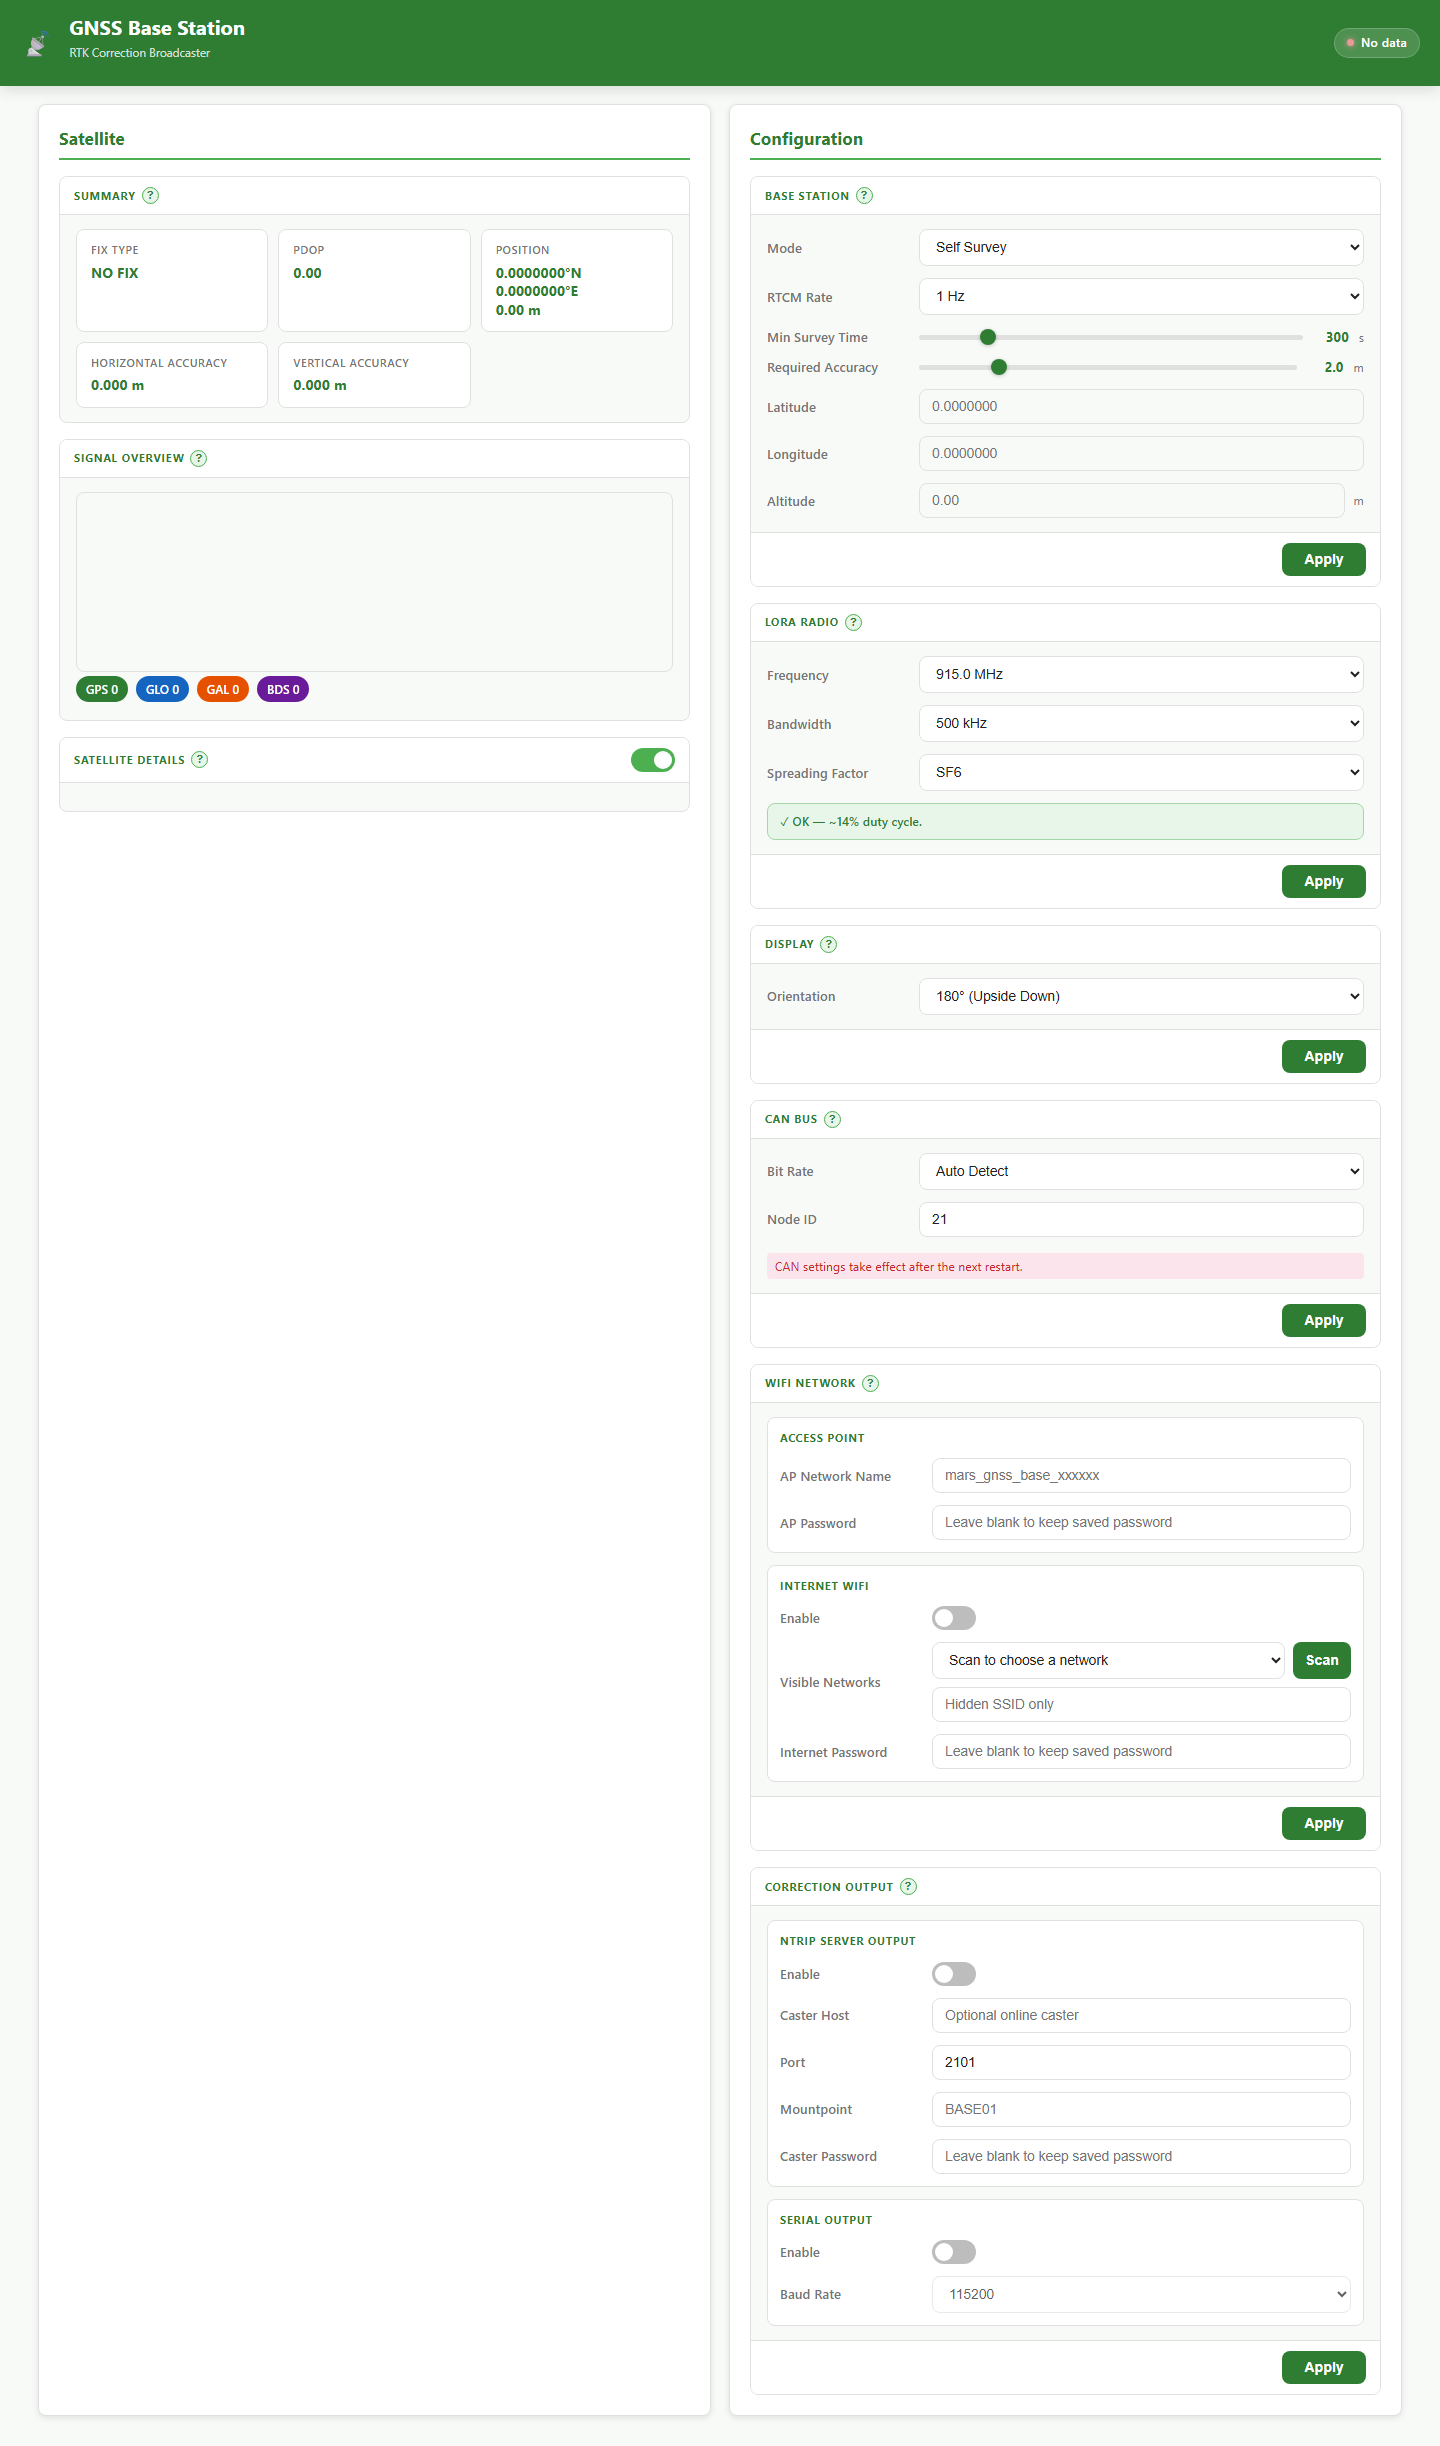
\includegraphics[keepaspectratio,alt={Actual GNSS Base Station webpage with satellite summary, survey, LoRa, display, CAN, Wi-Fi and correction output panels}]{assets/gps-base-web-ui.png}}
\caption{GNSS Base Station webpage. On a live base, satellite and survey
data replace the no-data placeholders.}
\end{figure}

\subsection{Open the base page}\label{open-the-base-page}

\begin{enumerate}
\tightlist
\item
  Mount the base antenna on a rigid point with the clearest available
  sky. Attach GNSS and RTK LoRa antennas before power.
\item
  Join \texttt{mars\_gnss\_base\_XXXXXX} using \texttt{alphaagtech},
  unless site credentials were changed.
\item
  Open \texttt{http://mars\_gnss\_base.local}. If mDNS is unavailable,
  open \texttt{http://192.168.10.1}.
\item
  Confirm the green page header is \textbf{GNSS Base Station}. Read Fix
  Type, PDOP, position, horizontal/vertical accuracy, signal chart,
  constellation counts, and optional satellite details.
\end{enumerate}

\subsection{Self Survey for a temporary/new base
point}\label{self-survey-for-a-temporarynew-base-point}

\begin{enumerate}
\tightlist
\item
  In \textbf{Base Station}, select \textbf{Self Survey}.
\item
  Select RTCM rate. Start with 1 Hz unless the approved radio-capacity
  plan supports a higher rate.
\item
  Set minimum survey time and required accuracy. Longer time and a
  tighter target generally take longer and still require an unobstructed
  sky.
\item
  Select \textbf{Apply}. The page reports \textbf{Survey started} and
  shows elapsed time/current accuracy.
\item
  Do not touch the antenna, tripod, cable, or ground reference. Wait for
  \textbf{Survey Complete}.
\item
  Verify the surveyed position. Firmware stores the precise ECEF result
  and changes the saved mode to Fixed Location so the base can reuse
  that point after restart.
\end{enumerate}

\subsection{Fixed Location for a known
point}\label{fixed-location-for-a-known-point}

\begin{enumerate}
\tightlist
\item
  Use only coordinates supplied by the site survey record. Select
  \textbf{Fixed Location}.
\item
  Choose \textbf{Manual Entry} and enter latitude, longitude, and
  altitude, or use \textbf{Time Average} only under the approved site
  method.
\item
  Check hemisphere/sign, datum, altitude reference, digits, and
  antenna-height convention. A plausible but wrong coordinate shifts
  every rover result.
\item
  Select \textbf{Apply}, then confirm the displayed position matches the
  record before allowing correction use.
\end{enumerate}

\subsection{Configure correction
outputs}\label{configure-correction-outputs}

\begin{enumerate}
\tightlist
\item
  In \textbf{LoRa Radio}, set frequency, bandwidth, and spreading factor
  to the approved RTK plan. The page's bandwidth-status line must say
  the selected link can carry the RTCM rate. Select Apply.
\item
  For a rover connected to the base AP by Wi-Fi, enable \textbf{NTRIP
  Server Output}, leave Caster Host blank, and set port/mountpoint. The
  rover uses the base AP address, normally \texttt{192.168.10.1}.
\item
  For an online caster, first enable \textbf{Internet WiFi}, scan/select
  the router and apply. Then enable NTRIP output and enter caster host
  without \texttt{http://}, port, mountpoint, and caster password.
\item
  For wired RTCM, enable \textbf{Serial Output} and select the receiving
  device's matching baud rate.
\item
  Do not use port 80 for NTRIP. Watch Stream Status and verify
  corrections at the rover rather than assuming Apply succeeded.
\end{enumerate}

\subsection{Other base controls}\label{other-base-controls}

{\def\LTcaptype{none} % do not increment counter
\begin{longtable}[]{@{}
  >{\raggedright\arraybackslash}p{(\linewidth - 2\tabcolsep) * \real{0.5000}}
  >{\raggedright\arraybackslash}p{(\linewidth - 2\tabcolsep) * \real{0.5000}}@{}}
\toprule\noalign{}
\begin{minipage}[b]{\linewidth}\raggedright
Panel
\end{minipage} & \begin{minipage}[b]{\linewidth}\raggedright
Instruction
\end{minipage} \\
\midrule\noalign{}
\endhead
\bottomrule\noalign{}
\endlastfoot
Display & Select the orientation that makes the onboard display upright;
Apply. \\
CAN Bus & Select \textbf{500 kbit/s} and a unique node ID. Default is
21. Auto Detect is a diagnostic option, not the commissioned
robot-system setting. Restart is required before CAN changes take
effect. \\
WiFi Access Point & Change AP name/password only during controlled
service. Record the new credentials before Apply; the phone may
disconnect when they change. \\
Satellite Details & Turn on for engineering diagnosis of constellation,
SNR, elevation/azimuth, correction and ephemeris data; turn off for a
simpler operator view. \\
\end{longtable}
}

\protect\phantomsection\label{gps-rover-web}
\section{GPS rover webpage and setup}\label{gps-rover-webpage-and-setup}

\begin{figure}
\centering
\pandocbounded{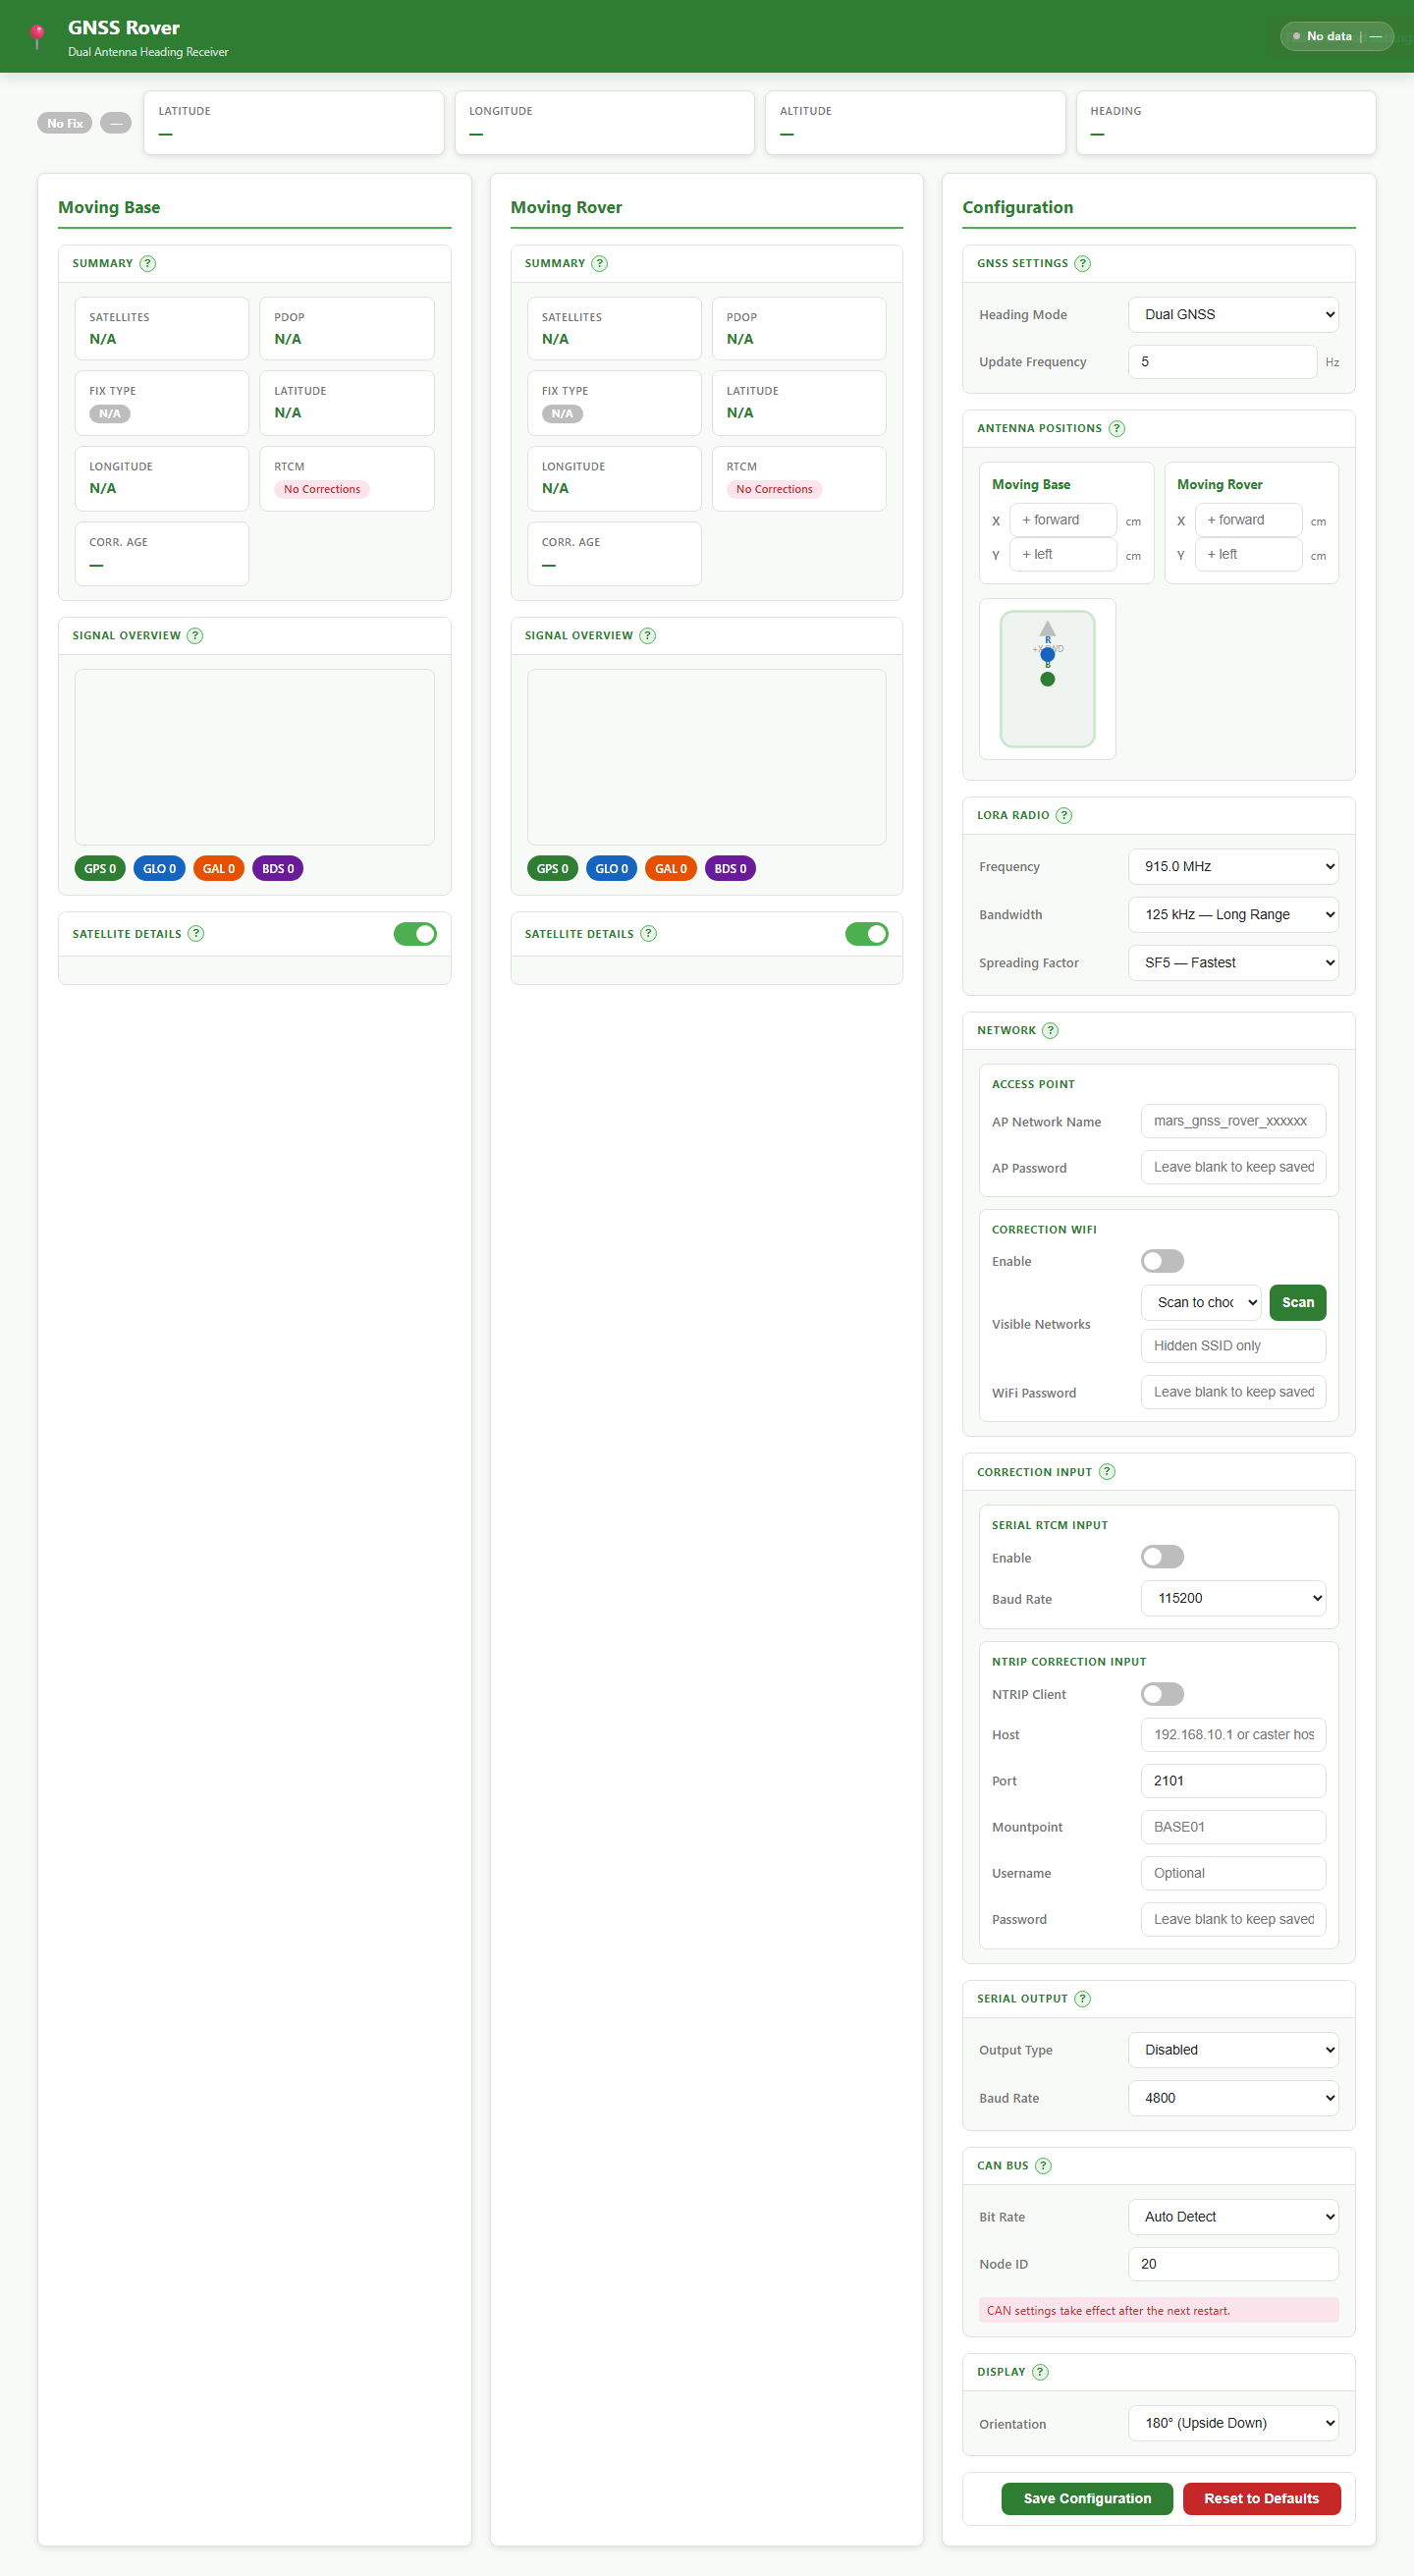
\includegraphics[keepaspectratio,alt={Actual GNSS Rover webpage with moving base and moving rover status, antenna positions, LoRa, network, correction input, serial, CAN and display settings}]{assets/gps-rover-web-ui.png}}
\caption{GNSS Rover webpage. The two satellite columns correspond to the
rover's Moving Base and Moving Rover receivers.}
\end{figure}

\subsection{Open and read the rover
page}\label{open-and-read-the-rover-page}

\begin{enumerate}
\tightlist
\item
  Keep the robot in Hold. Confirm both GNSS antennas, RTK LoRa antenna,
  and CAN cable are secure before power.
\item
  Join \texttt{mars\_gnss\_rover\_XXXXXX} with \texttt{alphaagtech},
  unless site credentials were changed.
\item
  Open \textbf{\texttt{http://mars\_gnss\_rover.local}}. Use
  \texttt{http://192.168.10.1} only as the direct-AP fallback.
\item
  Check the top solution badge and the \textbf{Moving Base} and
  \textbf{Moving Rover} summaries: satellites, PDOP, fix type,
  latitude/longitude, RTCM state, correction age, signal charts, and
  constellation counts.
\item
  Do not start Auto navigation unless the solution badge is OK, both
  receivers are plausible, corrections are fresh, and the site-required
  fix/accuracy is met.
\end{enumerate}

\subsection{GNSS mode and antenna
geometry}\label{gnss-mode-and-antenna-geometry}

\begin{enumerate}
\tightlist
\item
  Select \textbf{Dual GNSS} for the normal two-receiver position/heading
  calculation, or \textbf{Moving Baseline} only when the installed
  system and field procedure require it.
\item
  Set update frequency from 1--20 Hz. Factory default is 5 Hz; higher
  rates increase processing and serial bandwidth requirements.
\item
  Measure the center of each antenna relative to the robot reference
  point. Enter Moving Base X/Y and Moving Rover X/Y in centimeters,
  where +X is forward and +Y is left.
\item
  Check the diagram direction and signs. The calculation rejects invalid
  antenna geometry and a baseline under 20 cm; the webpage also warns
  below 10 cm at save time.
\item
  Select \textbf{Save Configuration}. After a mode/geometry change, keep
  the robot stationary and verify heading against a known direction
  before navigation.
\end{enumerate}

\subsection{Select and configure correction
input}\label{select-and-configure-correction-input}

{\def\LTcaptype{none} % do not increment counter
\begin{longtable}[]{@{}
  >{\raggedright\arraybackslash}p{(\linewidth - 4\tabcolsep) * \real{0.3333}}
  >{\raggedright\arraybackslash}p{(\linewidth - 4\tabcolsep) * \real{0.3333}}
  >{\raggedright\arraybackslash}p{(\linewidth - 4\tabcolsep) * \real{0.3333}}@{}}
\toprule\noalign{}
\begin{minipage}[b]{\linewidth}\raggedright
Method
\end{minipage} & \begin{minipage}[b]{\linewidth}\raggedright
Setup
\end{minipage} & \begin{minipage}[b]{\linewidth}\raggedright
Expected status
\end{minipage} \\
\midrule\noalign{}
\endhead
\bottomrule\noalign{}
\endlastfoot
RTK LoRa & Match base frequency, bandwidth and SF exactly; leave the
approved RC/RTK separation intact. & \textbf{LoRa corrections};
correction age remains current. \\
Base local NTRIP & Enable Correction WiFi; select the base AP; use host
\texttt{192.168.10.1}, base port/mountpoint and credentials; enable
NTRIP Client. & \textbf{NTRIP corrections}. \\
Online NTRIP caster & Enable Correction WiFi and join an Internet
router; enter caster host, port, mountpoint, username and password;
enable NTRIP Client. & NTRIP connects and corrections become fresh. \\
Serial RTCM & Disable NMEA Serial Output, enable Serial RTCM Input, and
match 4800--921600 baud to the sender. & \textbf{Serial corrections}. \\
\end{longtable}
}

\begin{manualwarning}

\textbf{Use one documented correction method for the job.} The firmware
can receive through several paths; avoid an ambiguous setup where
unrelated streams compete. The status field identifies the most recently
active path.

\end{manualwarning}

\subsection{CAN, serial output, display and
network}\label{can-serial-output-display-and-network}

\begin{enumerate}
\tightlist
\item
  Leave NMEA \textbf{Serial Output} disabled unless another device
  explicitly requires GPGGA. If enabled, choose a baud rate high enough
  for the GNSS update frequency; the page warns when it is too low.
\item
  For \textbf{CAN Bus}, select \textbf{500 kbit/s} and a unique node ID.
  Default rover ID is 20. Auto Detect is for diagnosis only. Save, then
  restart before expecting CAN changes.
\item
  Set Display Orientation so the onboard display is upright.
\item
  The rover configuration AP is always available. Correction WiFi is a
  separate client connection; changing one does not automatically change
  the other.
\item
  Use \textbf{Reset to Defaults} only under an authorized recovery
  procedure. It erases saved radio, antenna, correction, network, CAN,
  and display settings and requires complete recommissioning.
\end{enumerate}

\subsection{Meaning of rover solution
messages}\label{meaning-of-rover-solution-messages}

{\def\LTcaptype{none} % do not increment counter
\begin{longtable}[]{@{}
  >{\raggedright\arraybackslash}p{(\linewidth - 2\tabcolsep) * \real{0.5000}}
  >{\raggedright\arraybackslash}p{(\linewidth - 2\tabcolsep) * \real{0.5000}}@{}}
\toprule\noalign{}
\begin{minipage}[b]{\linewidth}\raggedright
Message
\end{minipage} & \begin{minipage}[b]{\linewidth}\raggedright
Meaning / response
\end{minipage} \\
\midrule\noalign{}
\endhead
\bottomrule\noalign{}
\endlastfoot
OK & Geometry calculation succeeded; still verify RTK fix, accuracy,
correction age and CAN delivery. \\
No fix & A receiver lacks a usable GNSS fix. Improve sky view and
wait. \\
Invalid coords & Input position is invalid; inspect GNSS data and
configuration. \\
UTM zone split & The two receiver coordinates fall in different UTM
zones; inspect coordinates and placement. \\
Baseline \textless20cm & Measured antenna separation is too short for
the solution. \\
Antenna cfg & Saved offsets are unset, too close, or inconsistent. \\
RelPos invalid / missing & Moving-baseline relative-position data is
invalid or absent; check mode, receivers, corrections and wiring. \\
\end{longtable}
}

\protect\phantomsection\label{gps-operation}
\section{GPS base and rover field
workflow}\label{gps-base-and-rover-field-workflow}

\begin{figure}
\centering
\pandocbounded{
\includegraphics[keepaspectratio,alt={Eight numbered GPS base and rover setup pictures}]{assets/gps-operation-guide.pdf}}
\caption{Use this field sequence after the detailed base and rover
webpage setup above.}
\end{figure}

\begin{enumerate}
\tightlist
\item
  \textbf{Place and identify the base.} Use the recorded base point and
  antenna height, or establish a new rigid point with clear sky.
\item
  \textbf{Power the base.} Attach antennas first. Open
  \texttt{mars\_gnss\_base.local} and verify the saved mode, position,
  corrections, and RTK radio plan.
\item
  \textbf{Complete position setup.} Finish Self Survey or verify Fixed
  Location. Do not move the antenna after this step.
\item
  \textbf{Verify correction output.} Confirm LoRa, NTRIP, or serial
  output is active using the selected field method.
\item
  \textbf{Power the robot rover.} Check the two GNSS antenna
  mounts/offsets, LoRa antenna, and CAN connection.
\item
  \textbf{Open \texttt{mars\_gnss\_rover.local}.} Verify mode, both
  receiver summaries, antenna geometry, chosen correction input, and
  fresh correction age.
\item
  \textbf{Verify the robot solution.} Require the site-approved RTK fix
  and accuracy, stable heading, OK solution status, and correct
  position/heading while the robot is stationary.
\item
  \textbf{Verify delivery.} Confirm rover node 20 and fresh GPS data at
  the robot and navigation console. Only then allow Auto; continue
  monitoring correction age and solution quality.
\end{enumerate}

\protect\phantomsection\label{gps-trouble}
\section{GPS troubleshooting}\label{gps-troubleshooting}

{\def\LTcaptype{none} % do not increment counter
\begin{longtable}[]{@{}
  >{\raggedright\arraybackslash}p{(\linewidth - 4\tabcolsep) * \real{0.3333}}
  >{\raggedright\arraybackslash}p{(\linewidth - 4\tabcolsep) * \real{0.3333}}
  >{\raggedright\arraybackslash}p{(\linewidth - 4\tabcolsep) * \real{0.3333}}@{}}
\toprule\noalign{}
\begin{minipage}[b]{\linewidth}\raggedright
Problem/status
\end{minipage} & \begin{minipage}[b]{\linewidth}\raggedright
What to inspect
\end{minipage} & \begin{minipage}[b]{\linewidth}\raggedright
Operator response
\end{minipage} \\
\midrule\noalign{}
\endhead
\bottomrule\noalign{}
\endlastfoot
\texttt{mars\_gnss\_base.local} or \texttt{mars\_gnss\_rover.local} does
not open & Wrong Wi-Fi, mDNS unsupported, changed AP credentials & Stay
joined to the device AP and use \texttt{192.168.10.1}. Confirm the page
title before editing. \\
Base survey never completes & Poor sky, antenna movement, multipath,
damaged cable, target too strict & Keep antenna rigid; improve sky view;
inspect hardware; restart the approved survey. \\
Base restarts at an unexpected position & Wrong fixed record or survey
point moved & Stop Auto. Compare displayed coordinates/ECEF-derived
position with site record; recommission the base. \\
Rover says No fix & One/both receivers lack usable GNSS & Move to open
sky, inspect both antennas/power, and wait. \\
Rover stays RTK Float or corrections age & Base invalid, LoRa
mismatch/interference, NTRIP/Internet failure, multipath & Check base
stream first; verify chosen correction path and radio separation;
improve sky view. \\
NTRIP waiting for WiFi & Correction WiFi disabled/not connected & Enable
it, scan/select the correct network, apply credentials, and recheck
status. \\
NTRIP missing host or mountpoint & Incomplete client settings & Enter
the exact host, port and mountpoint; do not include \texttt{http://}. \\
Baseline \textless20cm / Antenna cfg & Offsets or physical separation
wrong & Hold the robot; measure antennas; correct X/Y signs/units; save
and verify heading. \\
RelPos invalid or missing & Moving Baseline mode lacks valid relative
position & Verify mode, receiver operation, corrections and antenna
geometry. \\
Good rover page, no robot/navigation position & Wrong 500 kbit/s
setting, node ID, wiring or navigation path & Keep Hold; verify CAN port
pinout, live rover node, \textbf{500 kbit/s}, restart after CAN changes,
heartbeats and navigation topics. \\
CAN setting changed but no effect & Restart not completed & Record the
change, safely restart the device, then verify the live node and
\textbf{500 kbit/s} setting. \\
\end{longtable}
}

\chapter{Component · Automatic navigation
controller}\label{component-automatic-navigation-controller}

\protect\phantomsection\label{navigation}
\section{Navigation controller: component
overview}\label{navigation-controller-component-overview}

The navigation controller uses corrected GPS position and an
operator-planned route to command the robot. It is made of a
\textbf{Raspberry Pi 5 computer}, a \textbf{Pi camera connected to a
Raspberry Pi 5 CSI port}, and a \textbf{PoE module that provides its
power}. The robot's battery-powered PoE switch supplies the controller's
Ethernet/PoE connection. The operator uses a browser to draw the safe
boundary, create waypoints, upload the mission, start, pause, resume,
and monitor.

\begin{figure}
\centering
\pandocbounded{
\includegraphics[keepaspectratio,alt={Navigation controller containing Raspberry Pi 5, Pi camera connected to CSI, and PoE power module connected to the robot PoE switch}]{assets/navigation-controller-hardware.pdf}}
\caption{The navigation controller includes its Pi camera and connects
to the robot through PoE Ethernet and the power hub's 5 V CAN port.}
\end{figure}

\subsection{Features}\label{features-3}

\begin{itemize}
\tightlist
\item
  ROS Noetic navigation and dual-GNSS localization.
\item
  CAN communication with robot controller.
\item
  Map, waypoint, mission, geofence, status, and photo controls.
\item
  CSI-connected Pi camera H.264 live video through MediaMTX WebRTC.
\item
  PoE network and power connection from the robot PoE switch.
\item
  Mission pause on excessive localization uncertainty.
\item
  Geofence start refusal and automatic pause outside boundary.
\item
  Automatic navigation-service startup after the navigation controller
  boots; operators do not manually launch the normal service stack.
\item
  System monitoring, rosbridge, nginx web access, and managed service
  recovery.
\end{itemize}

\protect\phantomsection\label{nav-specs}
\section{Navigation-controller
specifications}\label{navigation-controller-specifications}

{\def\LTcaptype{none} % do not increment counter
\begin{longtable}[]{@{}
  >{\raggedright\arraybackslash}p{(\linewidth - 2\tabcolsep) * \real{0.5000}}
  >{\raggedright\arraybackslash}p{(\linewidth - 2\tabcolsep) * \real{0.5000}}@{}}
\toprule\noalign{}
\begin{minipage}[b]{\linewidth}\raggedright
Item
\end{minipage} & \begin{minipage}[b]{\linewidth}\raggedright
Specification
\end{minipage} \\
\midrule\noalign{}
\endhead
\bottomrule\noalign{}
\endlastfoot
Computer & Raspberry Pi 5 \\
Camera & Pi camera connected to a Raspberry Pi 5 CSI port \\
Power/network module & PoE module supplied by the robot PoE switch \\
PoE switch source & Robot battery power through the installed protected
supply path \\
Software &
\href{https://github.com/asilan/camera_catkin_ws/tree/video-stream}{camera\_catkin\_ws,
video-stream branch} \\
Production service & \texttt{camera.service} \\
Main launch file & \texttt{launch/camera.launch} \\
Expected Ethernet & \texttt{eth0} with IPv4 address \\
Operator-device network & Wi-Fi connection to \texttt{mars\_xxxxxx} for
the local robot webpage plus simultaneous cellular Internet for Google
map tiles \\
Robot bus & \texttt{can0} \\
ROS bridge & Local port 9090; browser secure proxy through nginx \\
Camera source & RTSP \texttt{127.0.0.1:8554/cam} \\
Browser video & WebRTC/WHEP at \texttt{/cam/whep}; media UDP 8189 \\
Default geofence buffer & 2 m outward \\
\end{longtable}
}

\protect\phantomsection\label{nav-connections}
\section{Navigation-controller external
connections}\label{navigation-controller-external-connections}

\begin{figure}
\centering
\pandocbounded{
\includegraphics[keepaspectratio,alt={Factory-assembled navigation controller with external PoE Ethernet and CAN connections}]{assets/navigation-controller-hardware.pdf}}
\caption{The Pi camera is part of the assembled navigation controller.
The controller's external robot connections are PoE Ethernet and the
power hub's 5 V CAN port.}
\end{figure}

\begin{manualnotice}

\textbf{Navigation-controller connections:} connect the labeled PoE
Ethernet cable to the robot PoE switch and connect the installed CAN
harness to the assigned power-hub 5 V CAN port. The Pi camera is already
part of the assembled controller.

\end{manualnotice}

{\def\LTcaptype{none} % do not increment counter
\begin{longtable}[]{@{}
  >{\raggedright\arraybackslash}p{(\linewidth - 4\tabcolsep) * \real{0.3333}}
  >{\raggedright\arraybackslash}p{(\linewidth - 4\tabcolsep) * \real{0.3333}}
  >{\raggedright\arraybackslash}p{(\linewidth - 4\tabcolsep) * \real{0.3333}}@{}}
\toprule\noalign{}
\begin{minipage}[b]{\linewidth}\raggedright
External connection
\end{minipage} & \begin{minipage}[b]{\linewidth}\raggedright
Purpose
\end{minipage} & \begin{minipage}[b]{\linewidth}\raggedright
Operator check
\end{minipage} \\
\midrule\noalign{}
\endhead
\bottomrule\noalign{}
\endlastfoot
Robot PoE switch -\textgreater{} navigation-controller PoE port &
\textbf{Operating power and Ethernet} & Correct labeled PoE port; cable
latched and undamaged; switch PoE/link indication present \\
Power-hub 5 V CAN port -\textgreater{} navigation-controller CAN
connector & Robot mode/status and Auto commands & Installed harness
connected to the labeled 5 V CAN port; pinout 5 V, CANH, CANL and GND;
500 kbit/s; correct termination; harness unmodified \\
Camera window/lens & Live view and recordings & Clean, unobstructed,
secure, and aimed correctly \\
Enclosure/cooling openings & Protects the assembled electronics &
Closed, dry, securely mounted, airflow clear \\
\end{longtable}
}

\subsection{External connection and startup
procedure}\label{external-connection-and-startup-procedure}

\begin{enumerate}
\tightlist
\item
  Keep the robot in Hold, UVC Off/Disarmed, contactor open, and power
  isolated.
\item
  Inspect the sealed navigation-controller enclosure. Do not open it or
  disturb its internal Pi camera, CSI ribbon, Raspberry Pi 5, or PoE
  module.
\item
  Connect the labeled PoE Ethernet cable from the robot PoE switch to
  the navigation-controller external PoE port. This is the
  controller\textquotesingle s operating-power path. Route it away from
  wheels, steering joints, lamp fixtures, ballast leads, and sharp
  edges.
\item
  Connect the installed CAN harness to its assigned power-hub 5 V CAN
  port. Verify the port pinout---1: 5 V, 2: CANH, 3: CANL, 4: GND---and
  confirm the connector is fully seated and the harness has not been
  altered. See the \hyperref[power-hub-ports]{power-hub port schedule}.
\item
  Secure both cables with strain relief, then restore robot power
  according to the startup procedure.
\item
  Allow the navigation controller to finish booting. Its navigation,
  web, ROS, camera/video, and supporting services start automatically;
  do not manually start the normal service stack.
\item
  Confirm the webpage becomes available, then verify PoE/link
  indicators, ROS Connected, live video, CAN status, and current RTK
  position. If the page or a service does not become ready, keep Hold
  and use the troubleshooting procedure.
\item
  If any check fails, return to Hold, isolate power, and correct the
  external connection. Internal enclosure service is for authorized
  technicians only.
\end{enumerate}

\protect\phantomsection\label{nav-operation}
\section{Automatic navigation operation
manual}\label{automatic-navigation-operation-manual}

\begin{manualwarning}

\textbf{Do not navigate from video alone.} Confirm RTK, map position,
robot health, the physical route, and emergency-stop coverage. Keep UVC
Off during first route validation.

\end{manualwarning}

\begin{figure}
\centering
\pandocbounded{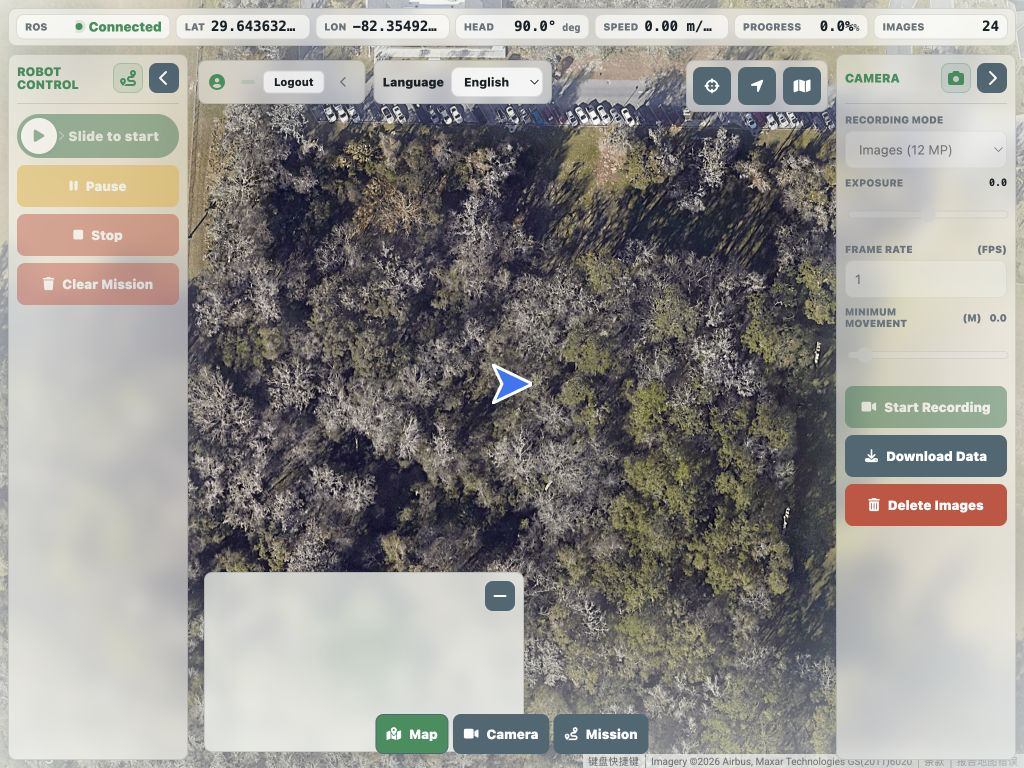
\includegraphics[keepaspectratio,alt={MARS navigation console Map view at 1024 by 760 pixels}]{assets/mars-console-map.png}}
\caption{Map view: monitor position and route while Robot Control and
Camera controls remain available.}
\end{figure}

\begin{figure}
\centering
\pandocbounded{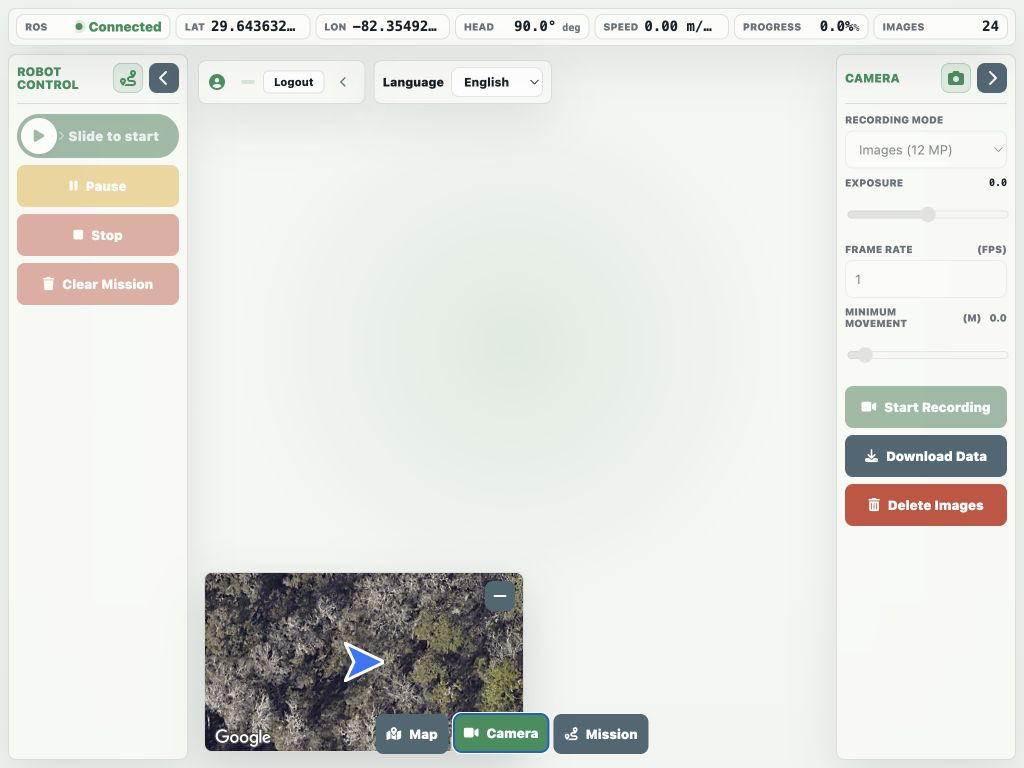
\includegraphics[keepaspectratio,alt={MARS navigation console Camera view at 1024 by 760 pixels}]{assets/mars-console-camera.png}}
\caption{Camera view: inspect the live video workspace while retaining
Robot Control and recording controls.}
\end{figure}

\begin{figure}
\centering
\pandocbounded{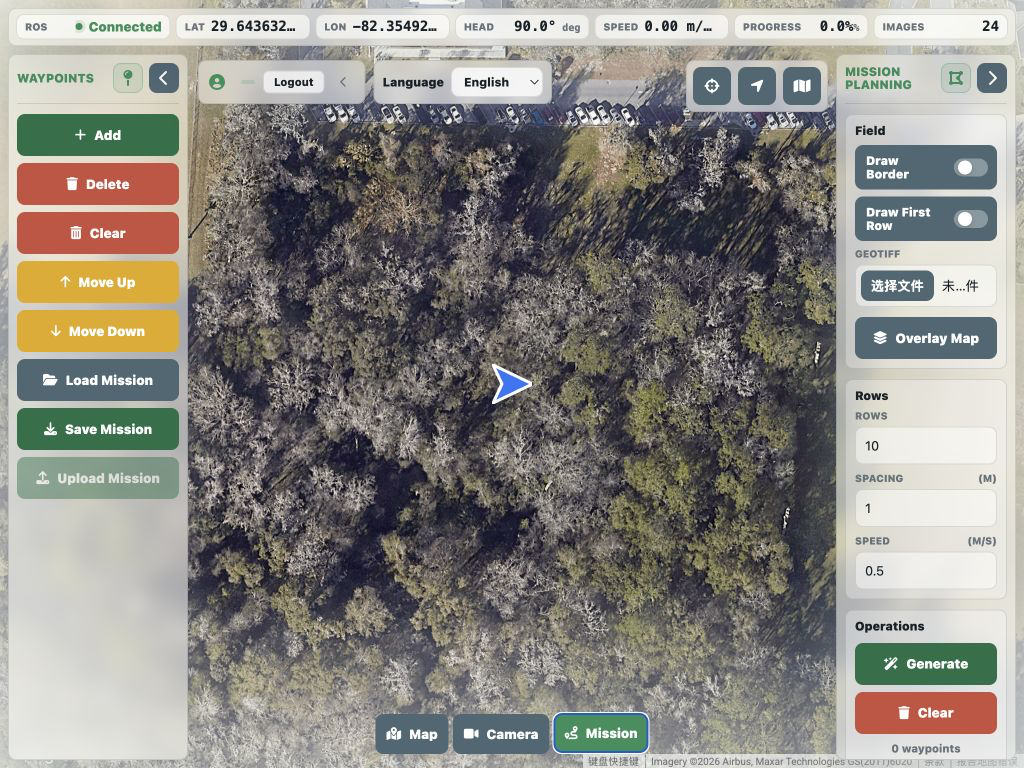
\includegraphics[keepaspectratio,alt={MARS navigation console Mission view at 1024 by 760 pixels}]{assets/mars-console-mission.png}}
\caption{Mission view: edit Waypoints on the left and configure field
rows and Mission Planning on the right.}
\end{figure}

\begin{manualnotice}

\textbf{Current web-interface behavior:} these instructions were
verified against the navigation workspace's pinned web release. The
console is designed for landscape orientation. On a phone or tablet,
rotate the device before operating.

\end{manualnotice}

\subsection{Create a navigation web account
(administrator)}\label{create-a-navigation-web-account-administrator}

\begin{manualwarning}

\textbf{Authorized administrators only.} The navigation webpage has no
Create Account button or self-registration. Create accounts from an
authorized SSH session while the robot is in Hold and UVC is
Off/Disarmed.

\end{manualwarning}

\begin{enumerate}
\tightlist
\item
  Connect to the navigation controller using the approved procedure in
  \hyperref[nav-technician-access]{Navigation controller: Wi-Fi and SSH
  access}, then sign in as the \texttt{mars} operating-system user.
\item
  Open the installed workspace: \texttt{cd\ /home/mars/mars\_server}.
\item
  Select the account role. Use \texttt{viewer} for
  map-and-telemetry-only access. Use \texttt{operator} only for trained
  personnel who may plan missions and claim robot control.
\item
  Choose a unique username and a strong, site-approved password. The
  account script validates the role but does not enforce password
  strength. Do not reuse the Wi-Fi, SSH, or another
  operator\textquotesingle s password.
\item
  Create the account with
  \texttt{/opt/robot-web-server/bin/python3\ scripts/create\_user.py\ \textless{}username\textgreater{}\ \textquotesingle{}\textless{}password\textgreater{}\textquotesingle{}\ \textless{}role\textgreater{}}.
  Replace \texttt{\textless{}role\textgreater{}} with exactly
  \texttt{operator} or \texttt{viewer}. Protect the terminal and command
  history according to site credential policy because the password is
  supplied as a command argument.
\item
  Require the confirmation
  \texttt{User\ \textquotesingle{}\textless{}username\textgreater{}\textquotesingle{}\ (\textless{}role\textgreater{})\ saved}.
  The server reloads the account file for each login, so a web-service
  restart is not required.
\item
  If the username already exists, this command replaces that
  account\textquotesingle s password and role. Coordinate the change and
  require the user to log out and sign in again; an existing browser
  session does not automatically receive a changed role.
\item
  Open \texttt{https://mars.local/} in a separate browser session,
  verify the new credentials and role badge, then log out. Do not claim
  control merely to test an account.
\item
  Run \texttt{exit} to close SSH and record the account creation or
  change in the controlled site log. Never record the password in the
  service report.
\end{enumerate}

\subsection{1 · Sign in and take operator
control}\label{sign-in-and-take-operator-control}

\begin{enumerate}
\tightlist
\item
  Power the robot in Hold and allow the navigation controller to
  complete boot. The navigation services start automatically; operators
  do not need to launch them. Join the approved robot/navigation network
  and open \texttt{https://mars.local/} or the commissioned web address.
\item
  Rotate a phone/tablet to landscape. Sign in with the assigned account.
  There is no browser self-registration; an administrator creates
  accounts.
\item
  A \textbf{Viewer} sees the map and telemetry only; Camera, Mission and
  the control panels are hidden. An \textbf{Operator} can plan
  waypoints, but robot/camera commands remain disabled until that
  session claims control.
\item
  Select \textbf{Claim Control}. Only one operator session can hold
  control. Claiming immediately transfers control from another operator
  without asking them, so coordinate first.
\item
  Do not reuse one account on two devices: a newer sign-in with the same
  username signs out the earlier session and releases its control.
\item
  Verify \textbf{ROS Connected}, plausible latitude/longitude, heading,
  speed, robot marker, live video, current RTK/localization, and no
  navigation fault. ROS Disconnected blocks navigation and recording
  commands.
\end{enumerate}

\subsection{2 · Set up a waypoint
mission}\label{set-up-a-waypoint-mission}

\begin{figure}
\centering
\pandocbounded{
\includegraphics[keepaspectratio,alt={Current Mission Planning controls for Draw Border, Draw First Row, GeoTIFF, rows, spacing, speed, Generate and Clear}]{assets/manual-planning-buttons.pdf}}
\caption{Current Mission Planning panel. Draw Border and Draw First Row
are mutually exclusive drawing modes.}
\end{figure}

\begin{enumerate}
\tightlist
\item
  Select \textbf{Mission}. This keeps the map in the center and opens
  the editable Mission Planning and Waypoints panels.
\item
  For a generated row path, enable \textbf{Draw Border} and tap at least
  three boundary points. Drag the editable polygon if correction is
  needed. Keep it inside verified safe terrain and away from obstacles,
  ditches, public access, water and unverified turns.
\item
  Enable \textbf{Draw First Row}; this turns Draw Border off. Tap point
  A and then B to define row direction. Drag A/B or tap a marker and
  enter precise latitude/longitude when needed.
\item
  Enter \textbf{Rows} (at least 1), \textbf{Spacing} in metres, and
  \textbf{Speed}. The generator creates alternating row directions and
  clips row endpoints to the field polygon.
\item
  Optionally choose a georeferenced \texttt{.tif}/\texttt{.tiff} and
  select \textbf{Overlay Map}. Treat it only as a planning aid and
  verify its alignment against known field features.
\item
  Select \textbf{Generate}. If draft waypoints already exist, confirm
  their replacement. Inspect every generated endpoint, connector, turn,
  order and clearance.
\item
  For manual map points, turn both drawing toggles Off, then tap the map
  at each desired location. The \textbf{Add} button is different: it
  adds one waypoint at the robot's current position and refuses when the
  GPS fix is missing or stale.
\item
  Drag waypoint markers only in Mission view. Tap one or more markers to
  select them. \textbf{Delete} removes selected points after
  confirmation; \textbf{Clear} removes all draft waypoints; \textbf{Move
  Up/Down} changes selected points in the route order.
\item
  The Waypoint Inspector edits every selected point. A blank field means
  the selected points have different values. Set latitude/longitude,
  speed 0.1--2.0 m/s, action, hold time, XY tolerance 0.01--5.0 m, and
  yaw tolerance 0.01--3.14 rad.
\item
  \textbf{None} passes the point without an action. \textbf{Take Photo}
  stops for the hold time and triggers a photo during the stop.
  \textbf{Stop \& Wait} stops for the hold time. Choosing either action
  gives a new point a default 5-second hold unless changed.
\item
  Select \textbf{Save Mission} to download the current draft as
  \texttt{mission.waypoints} in QGC WPL 110 format. It preserves speed
  changes and action/hold commands but does not save the live
  field-border/geofence polygon.
\item
  \textbf{Load Mission} accepts \texttt{.mission} and
  \texttt{.waypoints}, validates coordinates, ID and 0.1--2.0 m/s speed,
  and loads the result into the editable Mission draft. Loading neither
  uploads nor starts the robot. Redraw and verify the border before
  enabling a geofence.
\end{enumerate}

\subsection{3 · Upload, switch to Auto, and
start}\label{upload-switch-to-auto-and-start}

\begin{figure}
\centering
\pandocbounded{
\includegraphics[keepaspectratio,alt={Current Load Mission, Save Mission, Upload Mission, slide start, Pause, Stop, Clear Mission and waypoint editing controls}]{assets/manual-navigation-buttons.pdf}}
\caption{Upload transfers the reviewed draft and settings to the
navigation node. It does not move the robot. Slide to start begins
execution only after the robot is in Auto.}
\end{figure}

\begin{enumerate}
\tightlist
\item
  Keep the robot in Hold and stationary. Claim operator control; require
  ROS Connected and at least one valid draft waypoint.
\item
  Select \textbf{Upload Mission}. Review every listed point plus its
  coordinates, speed, action and hold. The dialog's default speed is
  only a fallback for a point without a valid individual speed.
\item
  Set default XY tolerance (0.01--5.0 m) and yaw tolerance (0.01--3.14
  rad). A waypoint-specific inspector value overrides its corresponding
  upload default.
\item
  Leave \textbf{Enable Geofence} checked for field operation. A live
  Draw Border polygon with at least three points is required;
  saved/loaded mission files do not restore it. Cancel and redraw the
  boundary if the page says it is missing.
\item
  Confirm Upload and wait for the success message. The uploaded
  navigation route and active geofence become the non-editable Map view;
  draft editing remains in Mission view.
\item
  Walk or visually inspect the route, clear the area, and place a
  trained operator at the physical emergency stop.
\item
  \textbf{Single Joystick Remote Controller:} long-press Button 2.
  \textbf{Dual Joystick Remote Controller:} long-press SW6. Wait for the
  controller and robot to report \textbf{Auto}; otherwise the navigation
  action is rejected.
\item
  Drag \textbf{Slide to start} fully to the right. Verify Target becomes
  waypoint 1, distance/progress begin updating, and the first physical
  movement is slow and correctly directed.
\item
  Supervise continuously. The dashed target line, current/reached
  waypoint colors, driven track, distance, progress, RTK/localization,
  robot mode, CAN, speed and messages must agree with the physical
  robot.
\end{enumerate}

\subsection{4 · Pause, resume, stop, and return to
Manual}\label{pause-resume-stop-and-return-to-manual}

\begin{manualnotice}

\textbf{Mode-change behavior:} switching the robot from Auto to either
\textbf{Manual} or \textbf{Hold} automatically stops active autonomous
navigation. The webpage Stop button is an additional direct way to
cancel the mission; it is not required before changing mode.

\end{manualnotice}

\begin{figure}
\centering
\pandocbounded{
\includegraphics[keepaspectratio,alt={Four illustrated steps showing webpage Pause or handheld Auto Pause, stopped-state verification, and Resume}]{assets/auto-pause-resume-guide.pdf}}
\caption{Selecting Auto Pause with Button 2 or SW6 pauses navigation
just like the webpage Pause button. The mission remains available to
resume after checks pass.}
\end{figure}

\begin{figure}
\centering
\pandocbounded{
\includegraphics[keepaspectratio,alt={Four illustrated steps showing Auto navigation, Button 1 or SW5 selecting Manual or Hold, automatic mission cancellation, and zero-motion verification}]{assets/auto-mode-exit-guide.pdf}}
\caption{Changing from Auto to Manual or Hold automatically stops
navigation. Always verify zero motion and that the console no longer
says Navigating.}
\end{figure}

\begin{enumerate}
\tightlist
\item
  For a controlled pause that keeps the mission available to resume,
  either select webpage \textbf{Pause} or change the robot mode from
  Auto to \textbf{Auto Pause}: short-press Button 2 on Single Joystick
  Remote Controller or SW6 on Dual Joystick Remote Controller. Both
  methods pause autonomous navigation. Confirm the webpage button
  changes to Resume, the displayed robot mode is Auto Pause, the status
  reads Paused, and the robot physically stops.
\item
  Read the exact message. A geofence exit produces a high-visibility
  safety pause; Resume is rejected until the robot is back inside.
  Correct stale odometry, high position error or other reported causes
  before continuing.
\item
  Select \textbf{Resume} or use the approved handheld Auto-Pause toggle.
  A successful service response returns the console to Navigating.
  Verify the next motion physically.
\item
  To end autonomous operation from the webpage, select \textbf{Stop}; it
  publishes a cancel request and ends active execution. To end it from a
  handheld, request \textbf{Manual} or \textbf{Hold}; either mode change
  automatically stops autonomous navigation.
\item
  After any stop method, confirm the robot is physically stationary,
  commanded speed is zero, and the webpage no longer reports Navigating
  before approaching, editing, or handing over control. \textbf{Clear
  Mission} removes the uploaded navigation route only when navigation is
  inactive; the Waypoints-panel Clear controls the editable draft.
\item
  Other signed-in consoles receive operator, mission and live navigation
  state changes. Do not interpret a remote state change as permission to
  operate; identify the responsible operator.
\item
  To regain joystick control, request Manual with Button 1 or SW5,
  verify both the robot/controller and webpage show that Auto navigation
  has stopped, then move the joystick slowly. Select Hold instead when
  no manual movement is required.
\item
  Select \textbf{Release Control} or Logout at handover. Logout and
  normal page close attempt to release the operator lock; always confirm
  the operator bar no longer shows your session as controller.
\end{enumerate}

\begin{manualnotice}

\textbf{Intended automatic behavior:} the robot follows waypoints in
list order, applies each waypoint's speed/tolerance/action, shows the
active target and driven track, pauses when commanded or when configured
safety/localization conditions fail, rejects out-of-geofence
start/resume, stops for an action's hold time, triggers Take Photo
during that stop, and presents an audible/visible completion or failure
dialog. The operator remains responsible for the surroundings and
emergency stop.

\end{manualnotice}

\protect\phantomsection\label{nav-internet}
\section{Use robot Wi-Fi and cellular Internet
together}\label{use-robot-wi-fi-and-cellular-internet-together}

\begin{manualnotice}

\textbf{Why both connections are needed:} the navigation webpage and
robot data are reached through the navigation controller's local Wi-Fi
access point. The Google map tiles come from the Internet. A cellular
phone or tablet must therefore remain connected to \texttt{mars\_xxxxxx}
by Wi-Fi while using 4G/LTE/5G cellular data for Internet traffic.

\end{manualnotice}

\begin{figure}
\centering
\pandocbounded{
\includegraphics[keepaspectratio,alt={Phone connected to mars\_xxxxxx by Wi-Fi for robot controls and to cellular data for Google Maps Internet access}]{assets/navigation-wifi-cellular-guide.pdf}}
\caption{Keep both paths active: Wi-Fi carries the local robot webpage,
video, status and commands; cellular data loads Google Maps. Do not
enable the phone's hotspot.}
\end{figure}

\begin{manualwarning}

\textbf{Before field use:} an active SIM/eSIM, cellular-data plan and
usable field signal are required. Cellular use may incur data or roaming
charges. Complete setup while the robot is stationary in Hold and UVC
Off/Disarmed.

\end{manualwarning}

\subsection{Android phone or cellular
tablet}\label{android-phone-or-cellular-tablet}

\begin{enumerate}
\tightlist
\item
  Before joining the robot, turn \textbf{Airplane mode Off} and
  \textbf{Mobile data On}. Open an ordinary Internet page to confirm
  that cellular data works, then close that page.
\item
  Open \textbf{Settings -\textgreater{} Network \& Internet
  -\textgreater{} Internet}, or \textbf{Settings -\textgreater{}
  Connections -\textgreater{} Wi-Fi} on Samsung devices. Select
  \texttt{mars\_xxxxxx} and enter \texttt{alphaaggech}.
\item
  The robot AP does not provide Internet. If Android reports \textbf{No
  Internet}, choose \textbf{Stay connected}, \textbf{Use this network as
  is}, or \textbf{Connect anyway}. Do not allow the phone to disconnect
  from the robot AP.
\item
  On a Samsung Galaxy device, open \textbf{Settings -\textgreater{}
  Connections -\textgreater{} Wi-Fi -\textgreater{} menu -\textgreater{}
  Intelligent Wi-Fi} and enable \textbf{Switch to mobile data}. A SIM is
  required, and the option can vary by model or carrier. On other
  Android devices, enable the equivalent cellular-fallback or
  adaptive-connectivity option if available.
\item
  If the phone provides per-app network controls, allow the browser to
  use \textbf{Wi-Fi or mobile data}. Disable Data Saver for the browser
  during operation if it prevents map loading.
\item
  Return to Wi-Fi settings and confirm \texttt{mars\_xxxxxx} still shows
  Connected, even if it also says No Internet. Do not switch to a
  different Wi-Fi network.
\end{enumerate}

\subsection{iPhone or cellular iPad}\label{iphone-or-cellular-ipad}

\begin{enumerate}
\tightlist
\item
  Open \textbf{Settings -\textgreater{} Cellular} or \textbf{Mobile
  Data}. Turn Cellular Data On, select the correct data line if Dual SIM
  is used, and allow cellular data for the browser.
\item
  On the same Cellular/Mobile Data page, scroll down and turn
  \textbf{Wi-Fi Assist} On. Wi-Fi Assist can use cellular data when the
  connected Wi-Fi has poor or no Internet service.
\item
  Open \textbf{Settings -\textgreater{} Wi-Fi}, select
  \texttt{mars\_xxxxxx}, and enter \texttt{alphaaggech}. Keep the blue
  checkmark on this network if iOS reports No Internet Connection.
\item
  Return to the browser. Wi-Fi Assist works with foreground apps and may
  not operate while data roaming, so verify the map before starting a
  mission.
\end{enumerate}

\subsection{Verify the two data paths}\label{verify-the-two-data-paths}

\begin{enumerate}
\tightlist
\item
  With Wi-Fi still connected to \texttt{mars\_xxxxxx}, open
  \texttt{https://mars.local/} and sign in. Confirm the robot status,
  camera and ROS connection load. This proves the local Wi-Fi path.
\item
  Open Map or Mission view. Pan or zoom slightly and confirm Google road
  or satellite tiles appear instead of a blank gray background. This
  proves the cellular Internet path.
\item
  Recheck the phone status: Wi-Fi must remain connected to
  \texttt{mars\_xxxxxx}, and the cellular indicator must show usable
  service. Do not begin planning until both paths work.
\item
  Keep the browser in the foreground, the phone charged, and both
  connections enabled throughout navigation. Recheck after any loss of
  map, video, ROS or robot status.
\end{enumerate}

\subsection{Connection
troubleshooting}\label{connection-troubleshooting}

{\def\LTcaptype{none} % do not increment counter
\begin{longtable}[]{@{}
  >{\raggedright\arraybackslash}p{(\linewidth - 4\tabcolsep) * \real{0.3333}}
  >{\raggedright\arraybackslash}p{(\linewidth - 4\tabcolsep) * \real{0.3333}}
  >{\raggedright\arraybackslash}p{(\linewidth - 4\tabcolsep) * \real{0.3333}}@{}}
\toprule\noalign{}
\begin{minipage}[b]{\linewidth}\raggedright
Symptom
\end{minipage} & \begin{minipage}[b]{\linewidth}\raggedright
Likely cause
\end{minipage} & \begin{minipage}[b]{\linewidth}\raggedright
Action
\end{minipage} \\
\midrule\noalign{}
\endhead
\bottomrule\noalign{}
\endlastfoot
Robot webpage works, but Google map is gray & Cellular data is Off,
cellular fallback is disabled, browser cellular access is blocked, no
field signal, data limit reached, or roaming prevents fallback & Keep
robot Wi-Fi connected. Verify mobile data, signal, plan/roaming policy
and browser permission; enable Switch to mobile data or Wi-Fi Assist;
reload the page. \\
Google Maps works, but \texttt{mars.local} does not & The phone left
\texttt{mars\_xxxxxx}, selected another Wi-Fi network, or VPN/private
DNS blocks local addressing & Reconnect to \texttt{mars\_xxxxxx} and
choose Stay connected. Disable automatic switching to better Wi-Fi.
Pause an approved VPN/private-DNS service only if site policy permits,
then retry. \\
Phone repeatedly drops the robot AP & The device rejects a Wi-Fi network
without Internet or prefers another saved network & Select Connect
anyway/Stay connected, disable automatic joining of nearby networks for
the operation, and verify \texttt{mars\_xxxxxx} before every command. \\
Turning on hotspot disconnects the robot & The phone cannot remain a
Wi-Fi client while serving its own hotspot & Turn the hotspot Off and
reconnect to \texttt{mars\_xxxxxx}. Use cellular data directly on the
operating device. \\
No dual-path option is available & Device, carrier or policy does not
support simultaneous local Wi-Fi and cellular fallback & Use an approved
cellular-capable phone/tablet that supports both paths. Do not operate
with an unverified or blank map. \\
\end{longtable}
}

Phone menus vary by operating-system version, model and carrier.
Platform references:
\href{https://www.samsung.com/us/support/answer/ANS10002546/}{Samsung
Intelligent Wi-Fi} and
\href{https://support.apple.com/en-us/102228}{Apple Wi-Fi Assist}.

\protect\phantomsection\label{nav-web}
\section{Navigation webpage: current operator
controls}\label{navigation-webpage-current-operator-controls}

\begin{manualnotice}

\textbf{Simulation notice:} These interface screenshots are simulated
examples created for this manual. Actual map imagery, robot position,
status values, camera content, and interface appearance may differ
during operation.

\end{manualnotice}

\begin{figure}
\centering
\pandocbounded{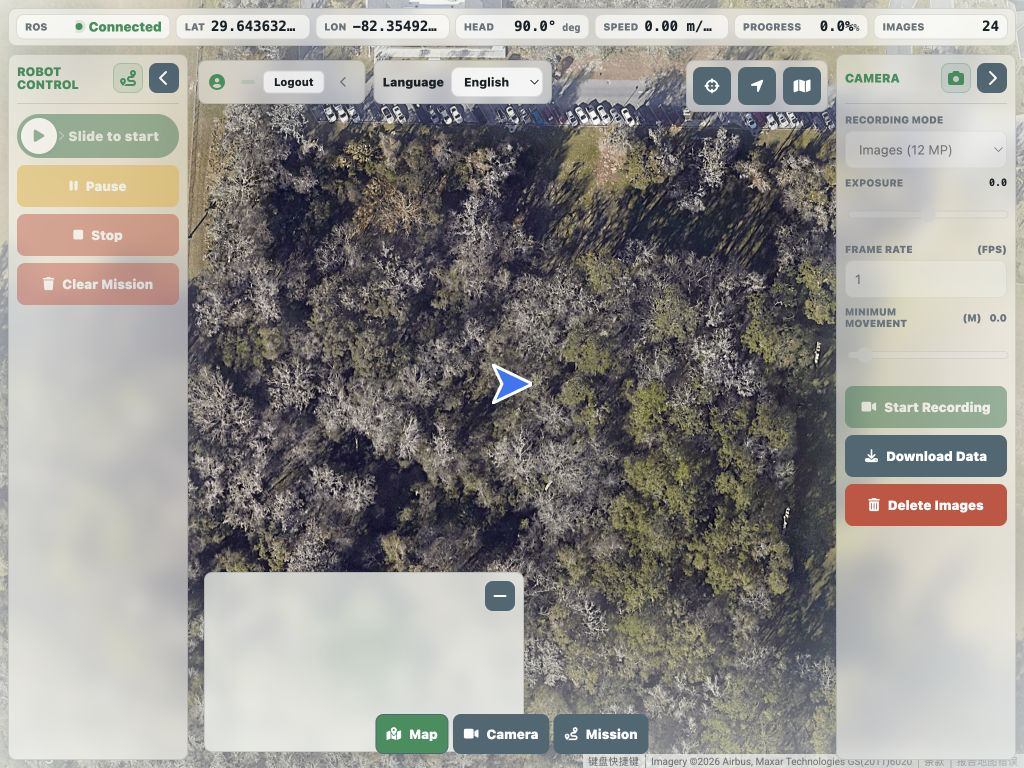
\includegraphics[keepaspectratio,alt={Current MARS Robot Console Map layout at 1024 by 760 pixels}]{assets/mars-console-map.png}}
\caption{Map page with the top status strip, Robot Control panel, map
controls, camera preview, and Camera panel.}
\end{figure}

\begin{figure}
\centering
\pandocbounded{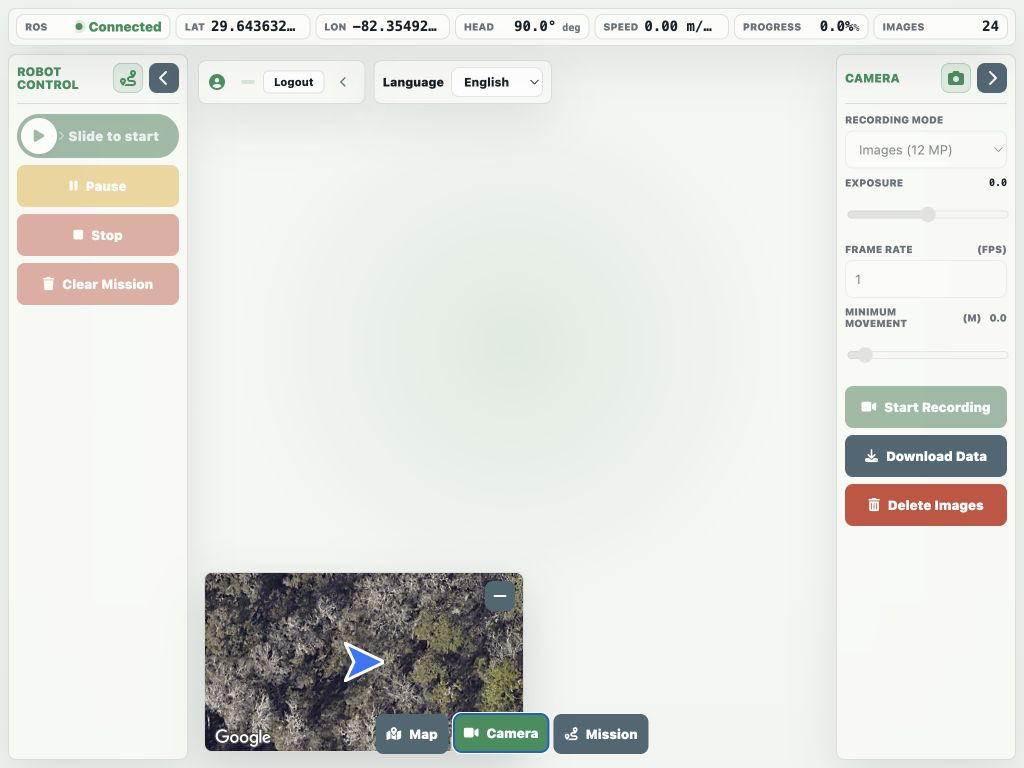
\includegraphics[keepaspectratio,alt={Current MARS Robot Console Camera layout at 1024 by 760 pixels}]{assets/mars-console-camera.png}}
\caption{Camera page with the main video workspace, small map preview,
Robot Control panel, and recording controls.}
\end{figure}

\begin{figure}
\centering
\pandocbounded{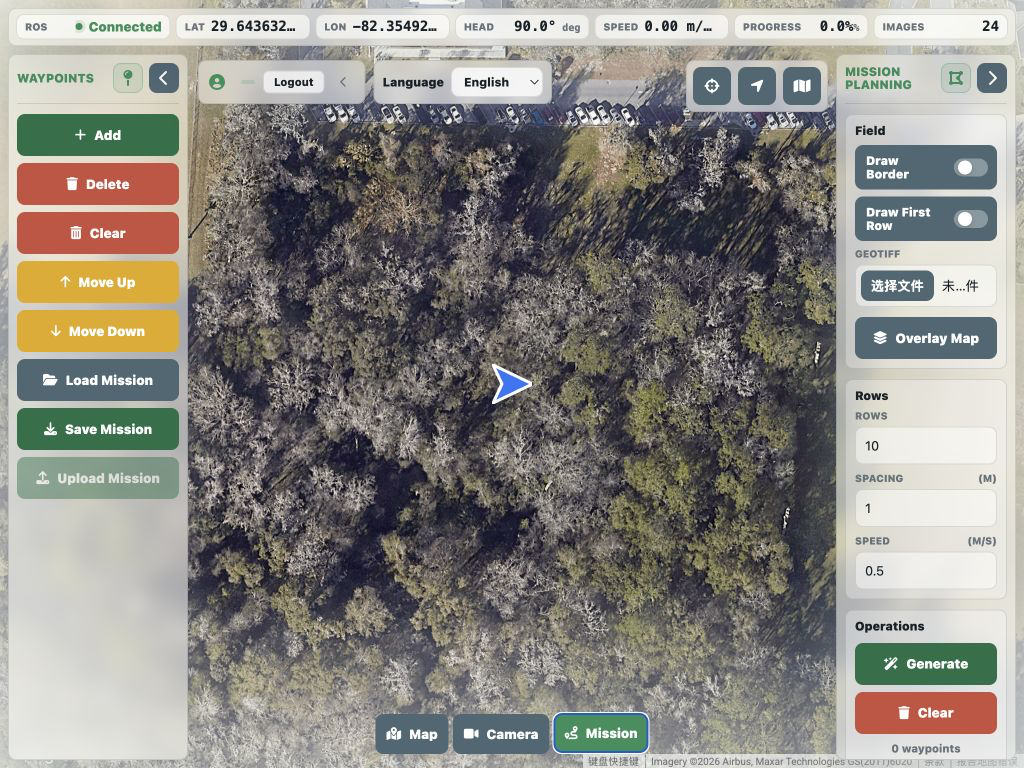
\includegraphics[keepaspectratio,alt={Current MARS Robot Console Mission layout at 1024 by 760 pixels}]{assets/mars-console-mission.png}}
\caption{Mission page with Waypoints, editable map workspace, and
Mission Planning controls. The console requires landscape orientation.}
\end{figure}

{\def\LTcaptype{none} % do not increment counter
\begin{longtable}[]{@{}
  >{\raggedright\arraybackslash}p{(\linewidth - 4\tabcolsep) * \real{0.3333}}
  >{\raggedright\arraybackslash}p{(\linewidth - 4\tabcolsep) * \real{0.3333}}
  >{\raggedright\arraybackslash}p{(\linewidth - 4\tabcolsep) * \real{0.3333}}@{}}
\toprule\noalign{}
\begin{minipage}[b]{\linewidth}\raggedright
Area/control
\end{minipage} & \begin{minipage}[b]{\linewidth}\raggedright
Current behavior
\end{minipage} & \begin{minipage}[b]{\linewidth}\raggedright
Operator use
\end{minipage} \\
\midrule\noalign{}
\endhead
\bottomrule\noalign{}
\endlastfoot
Orientation message & Blocks the portrait phone layout and requests
landscape & Rotate before planning or operating. \\
Top status strip & ROS connection, latitude, longitude, heading, speed,
mission progress and image count & Require Connected and plausible fresh
values before commands. \\
Map & Main map plus small live-camera preview; shows robot, driven
track, uploaded route, current target and active geofence & Supervise
route and physical position together. \\
Center on robot & Centers the map on fresh robot GPS & Use when the
robot marker is off-screen; a stale/missing fix is rejected. \\
Center on this device & Uses the phone/laptop browser geolocation &
Allow location permission only when useful; it does not change robot
localization. \\
Map-type button & Toggles roadmap and satellite map & Choose the view
that best exposes field features; neither is a safety survey. \\
Camera & Main live WebRTC video plus a small robot-centered map preview
& Inspect framing and use tap-to-focus/expose; never navigate from video
alone. \\
Preview minus/restore & Minimizes or restores the small camera/map
preview & Use to clear screen space without stopping either data
path. \\
Mission & Shows the shared map with editable draft waypoints and the
Mission Planning panel & Create/edit only while navigation is
inactive. \\
Panel chevrons & Collapse/restore Robot Control, Waypoints, Camera and
Mission Planning panels & Use for screen space; re-open the panel before
its controls are needed. \\
Fullscreen & Requests browser fullscreen where supported & Useful on
phones/tablets; browser/home-screen support varies. \\
Language & English, Chinese or Spanish; saved in that browser & Select a
language the operator reads reliably. \\
Operator bar & Username, role, Claim Control, Release Control and
Logout; can collapse & Verify who holds control before every command. \\
Robot Control readout & Target waypoint, distance, status and progress &
Compare with the top strip, map and physical robot. \\
Load Mission & Loads \texttt{.mission} CSV or QGC WPL
\texttt{.waypoints} into the editable Mission draft & Validate and
review; load does not upload or start. \\
Save Mission & Current button downloads draft as
\texttt{mission.waypoints} (QGC WPL 110) & Save after review. Redraw the
field border after reload because the geofence is not stored. \\
Upload Mission & Requires operator control and ROS; reviews point
properties/default tolerances and optional live-border geofence & Upload
only after physical route review; disabled while navigating. \\
Slide to start & Sends the execute-mission action after upload & Use
only with robot confirmed Auto and area clear. \\
Pause / Resume & The webpage Pause calls the pause service. Changing the
robot from Auto to Auto Pause with Button 2 or SW6 also pauses
navigation and retains the mission. Resume continues only after a
successful response. & Confirm zero motion and Paused/Auto Pause.
Correct a rejection, geofence, localization, or other pause cause before
Resume. \\
Stop & Publishes mission cancellation & Directly cancels navigation.
Changing robot mode from Auto to Manual or Hold also stops navigation
automatically. \\
Clear Mission & Clears the uploaded navigation route when inactive &
Different from Waypoints Clear, which clears the draft. \\
Add & Adds one draft point at the robot's current position; requires a
fresh GPS fix & Use when physically placing waypoints with the robot. \\
Map tap in Mission & With both drawing toggles Off, adds a draft
waypoint at the tapped location & Use for manual map-based route
construction. \\
Delete / draft Clear & Deletes selected draft points or all draft points
after confirmation & Confirm the count and route after removal. \\
Move Up / Down & Moves selected draft points one position while
preserving multi-selection order & Recheck the red connecting line after
every reorder. \\
Waypoint Inspector & Edits all selected points; blank means mixed values
& Set coordinates, speed, action/hold and optional point tolerances. \\
Draw Border / First Row & Mutually exclusive map modes; border is
editable/draggable, A/B markers are draggable & Required for row
generation; border is also the live geofence source at upload. \\
Rows / Spacing / Speed / Generate & Builds alternating lines clipped to
the polygon & Review every turn and row endpoint after generation. \\
GeoTIFF / Overlay Map & Loads local georeferenced TIFF as a planning
overlay & Optional; verify projection and alignment. \\
Planning Clear & Removes draft border, A/B line, overlay and draft
waypoints after confirmation & Does not substitute for Stop or Clear
Mission. \\
\end{longtable}
}

\begin{manualwarning}

\textbf{Draft versus uploaded route:} Mission view edits
\emph{planningWaypoints}. A successful Upload copies that reviewed draft
into the active navigation route. Map view shows the active route.
Saving stores draft waypoint commands but not the live border/geofence.
Keep this distinction clear during handover.

\end{manualwarning}

\subsection{Record still images}\label{record-still-images}

\begin{figure}
\centering
\pandocbounded{
\includegraphics[keepaspectratio,alt={Current Images and Video modes, exposure, frame rate, movement, Start Recording, Download Data and Delete Images controls}]{assets/manual-camera-buttons.pdf}}
\caption{Current camera panel. Frame Rate and Min. Movement are
image-only controls and become disabled in Video mode.}
\end{figure}

\begin{enumerate}
\tightlist
\item
  Claim operator control and confirm ROS Connected, live video,
  available storage, clean lens and correct aim.
\item
  Select \textbf{Camera} so video is the main stage. In Recording Mode
  choose \textbf{Images (12 MP)}; stills are fixed at 4608 × 2592.
\item
  Set Exposure from −5 to +5 as required. Tap/click inside the actual
  video frame to request autofocus and auto-exposure at that point. The
  request is ignored in the small preview, without operator control,
  without ROS, or when tapping the letterbox outside the image.
\item
  Set Frame Rate from 0.1 to 2 images/s and Min. Movement from 0 to 1 m.
  A new still is gated by these settings; 0 m disables the movement
  separation.
\item
  Select \textbf{Start Recording}. Wait for a success message and the
  button to change to Stop Recording. Confirm Images count rises as
  expected; live preview may fall to about 14 fps during full-resolution
  still capture.
\item
  Select \textbf{Stop Recording} and wait for success before changing
  mode, downloading or shutting down.
\end{enumerate}

\subsection{Record video}\label{record-video}

\begin{enumerate}
\tightlist
\item
  Stop any current still recording, then select \textbf{Video (30 fps)}.
  Video records the 2304 × 1296 live stream as MP4; Frame Rate and Min.
  Movement are disabled because they do not apply.
\item
  Set exposure and verify the main live frame. Tap-to-focus/expose
  remains available with operator control and ROS.
\item
  Select \textbf{Start Recording}. Wait for success and verify the Stop
  Recording state.
\item
  Select \textbf{Stop Recording} before changing modes, leaving the job
  or removing power. Wait for the service success response so the MP4
  can close correctly.
\end{enumerate}

\subsection{Download or delete
recordings}\label{download-or-delete-recordings}

\begin{enumerate}
\tightlist
\item
  Stop recording first and confirm the Stop Recording state.
\item
  Select \textbf{Download Data}. The picker lists collection sections
  with separate image/video counts. Select one section; Download stays
  disabled until a section is selected.
\item
  Select \textbf{Download}. The server prepares or reuses a ZIP and
  shows compression progress. Keep the page and network connection open
  until the browser download begins and completes.
\item
  Open the ZIP, compare the section name/counts and spot-check images
  and MP4 files before deleting robot data.
\item
  For authorized cleanup, select \textbf{Delete Images}. Despite the
  label, deletion selects one or more complete collection sections and
  removes their stored contents, including videos. Confirm the selected
  count carefully.
\item
  Wait for the success message. Deletion is not a backup and may not be
  recoverable.
\end{enumerate}

\begin{manualnotice}

\textbf{Geofence behavior:} the enforced polygon uses the Plan border
expanded outward 2 m by default. Starting outside it is refused. Leaving
it during navigation pauses the mission, and Resume is rejected until
the robot returns inside.

\end{manualnotice}

\protect\phantomsection\label{nav-trouble}
\section{Auto-navigation
troubleshooting}\label{auto-navigation-troubleshooting}

{\def\LTcaptype{none} % do not increment counter
\begin{longtable}[]{@{}
  >{\raggedright\arraybackslash}p{(\linewidth - 2\tabcolsep) * \real{0.5000}}
  >{\raggedright\arraybackslash}p{(\linewidth - 2\tabcolsep) * \real{0.5000}}@{}}
\toprule\noalign{}
\begin{minipage}[b]{\linewidth}\raggedright
Problem
\end{minipage} & \begin{minipage}[b]{\linewidth}\raggedright
What to do
\end{minipage} \\
\midrule\noalign{}
\endhead
\bottomrule\noalign{}
\endlastfoot
camera.service inactive & Keep robot in Hold. Service staff check
\texttt{systemctl\ status\ camera.service} and
\texttt{journalctl\ -u\ camera.service\ -n\ 80\ -\/-no-pager}, then
inspect power/network/storage/build. \\
Webpage opens, video shows 502 & Nginx cannot reach MediaMTX; check
\texttt{mediamtx.service}. \\
``No stream available on path cam'' & MediaMTX is running but camera
node is not pushing. Check camera ribbon, permission, camera service,
and logs. \\
Video connects but stays blank & Check UDP 8189 path between browser and
robot. \\
Mission will not start & Check robot inside geofence, Auto mode,
valid/current RTK odometry, CAN, uploaded mission, and emergency
state. \\
Mission pauses & Read the exact message. Correct high covariance, stale
odometry, CAN loss, or geofence exit before Resume. \\
\end{longtable}
}

\protect\phantomsection\label{nav-technician-access}
\section{Navigation controller: Wi-Fi and SSH
access}\label{navigation-controller-wi-fi-and-ssh-access}

\begin{manualwarning}

\textbf{Authorized field technicians only.} Before connecting, select
Hold, restrain the drive wheels for command-path testing, physically
disconnect UVC power, and keep the emergency stop available. A terminal
command can stop services or cause robot commands; begin with the
read-only checks below.

\end{manualwarning}

\begin{figure}
\centering
\pandocbounded{
\includegraphics[keepaspectratio,alt={Six illustrated steps for safely joining the navigation controller Wi-Fi access point and connecting by SSH}]{assets/navigation-technician-access.pdf}}
\caption{Technician access path: safe state -\textgreater{} join the
correct AP -\textgreater{} use \protect\texttt{mars.local}
-\textgreater{} SSH as \protect\texttt{mars} -\textgreater{} inspect
-\textgreater{} exit and recommission.}
\end{figure}

\subsection{Access credentials and
addressing}\label{access-credentials-and-addressing}

{\def\LTcaptype{none} % do not increment counter
\begin{longtable}[]{@{}
  >{\raggedright\arraybackslash}p{(\linewidth - 4\tabcolsep) * \real{0.3333}}
  >{\raggedright\arraybackslash}p{(\linewidth - 4\tabcolsep) * \real{0.3333}}
  >{\raggedright\arraybackslash}p{(\linewidth - 4\tabcolsep) * \real{0.3333}}@{}}
\toprule\noalign{}
\begin{minipage}[b]{\linewidth}\raggedright
Item
\end{minipage} & \begin{minipage}[b]{\linewidth}\raggedright
Installed/default value
\end{minipage} & \begin{minipage}[b]{\linewidth}\raggedright
Field note
\end{minipage} \\
\midrule\noalign{}
\endhead
\bottomrule\noalign{}
\endlastfoot
Navigation-controller Wi-Fi AP & \texttt{mars\_XXXXXX} & \texttt{XXXXXX}
is the unit-specific suffix. Confirm the label/serial number so a
technician does not join another nearby robot. \\
Navigation-controller AP password & \texttt{alphaaggech} & This
navigation-controller value is spelled with \textbf{ggech}. Enter it
exactly as shown. \\
General device AP default & \texttt{alphaagtech} & Use for other
robot-system device APs unless that component\textquotesingle s table or
site record gives a device-specific value. It is different from the
navigation-controller password above. \\
SSH hostname & \texttt{mars.local} & Primary technician target while
connected to the navigation-controller network. \\
SSH user & \texttt{mars} & The deployed service runs as user/group
\texttt{mars} and the workspace is under \texttt{/home/mars}. \\
SSH password & Site-issued operating-system account password & The Wi-Fi
AP password is not automatically the SSH password. Obtain the OS
credential through the site\textquotesingle s credential record; do not
guess or place it in a service report. \\
IP fallback & AP default-gateway address or commissioned address & Use
only when \texttt{mars.local} does not resolve. Read the connected Wi-Fi
adapter\textquotesingle s default gateway and record it as
\texttt{\textless{}NAV\_IP\textgreater{}}. \\
\end{longtable}
}

\begin{manualnotice}

\textbf{Password precedence:} the specific navigation-controller AP
credential above overrides the general device default. If a commissioned
unit no longer accepts a default, use the site credential record; do not
factory-reset it in the field merely to restore a published password.

\end{manualnotice}

\subsection{Connect a technician laptop to the navigation-controller
AP}\label{connect-a-technician-laptop-to-the-navigation-controller-ap}

\begin{enumerate}
\tightlist
\item
  Keep the robot in Hold, verify zero motion, disconnect UVC power, and
  tell the responsible operator that technician access is starting.
\item
  On the laptop, open Wi-Fi networks and select the exact
  \texttt{mars\_XXXXXX} matching the robot being serviced.
\item
  Enter \texttt{alphaaggech}. Remain connected if the laptop reports
  \textbf{No Internet}; this is a local service network.
\item
  Use \texttt{mars.local} as the navigation-controller hostname. Confirm
  the Wi-Fi SSID is still the intended robot before opening a browser or
  terminal.
\item
  If \texttt{mars.local} does not resolve, find the AP default gateway.
  On Windows run \texttt{ipconfig}; on Linux run \texttt{ip\ route}; on
  macOS run \texttt{route\ -n\ get\ default}. Record the gateway as
  \texttt{\textless{}NAV\_IP\textgreater{}} for the fallback SSH
  command.
\end{enumerate}

\subsection{Open an SSH session}\label{open-an-ssh-session}

\begin{enumerate}
\tightlist
\item
  Open Windows Terminal/PowerShell, macOS Terminal, or a Linux terminal.
\item
  Run \texttt{ssh\ mars@mars.local}. If the local name does not resolve,
  run \texttt{ssh\ mars@\textless{}NAV\_IP\textgreater{}} using the AP
  gateway or commissioned IP found above.
\item
  On the first connection, compare the displayed SSH host-key
  fingerprint with the commissioned fingerprint or maintenance record.
  Accept it only when the robot identity and fingerprint are verified.
  An unexpected key change can indicate a replaced controller,
  reinstalled OS, wrong robot, or security problem.
\item
  Enter the site-issued \texttt{mars} operating-system password when
  prompted. The terminal does not display dots or characters while the
  password is typed; this is normal.
\item
  Confirm the prompt identifies the intended unit. Run
  \texttt{hostname}, \texttt{hostname\ -I}, and \texttt{whoami}.
  Expected hostname is \texttt{mars} and expected user is \texttt{mars};
  compare the addresses with the unit record.
\end{enumerate}

\subsection{Read-only first
inspection}\label{read-only-first-inspection}

\begin{verbatim}
hostname
hostname -I
whoami
uptime
git -C /home/mars/camera_catkin_ws branch --show-current
git -C /home/mars/camera_catkin_ws rev-parse --short HEAD
systemctl status camera.service --no-pager
journalctl -u camera.service -n 80 --no-pager
ip -4 addr show eth0
ip -details link show can0
df -h /home/mars
vcgencmd get_throttled
vcgencmd measure_temp
\end{verbatim}

Expected results are the approved hostname/IP, user \texttt{mars},
branch \texttt{video-stream}, recorded commit, \texttt{camera.service}
active, \texttt{eth0} configured, \texttt{can0} UP at the commissioned
500 kbit/s, adequate free storage, no active undervoltage/throttling,
and acceptable temperature. Record the output before changing
configuration or restarting a service.

\subsection{End the session and return the system to
service}\label{end-the-session-and-return-the-system-to-service}

\begin{enumerate}
\tightlist
\item
  Do not leave an unattended administrator terminal connected. Finish
  the approved work and save the service record.
\item
  Run \texttt{exit} and confirm the SSH session closes. Disconnect the
  laptop from \texttt{mars\_XXXXXX}.
\item
  Complete \hyperref[nav-engineer]{post-service commissioning}: verify
  the production service, web console, live video, RTK localization,
  CAN, Hold/Auto gating, Pause/Resume, geofence, and physical emergency
  stop.
\item
  Remove wheel restraint and restore UVC power only after the
  responsible operator accepts the complete system and every
  cover/connection is restored.
\end{enumerate}

\subsection{SSH troubleshooting}\label{ssh-troubleshooting}

{\def\LTcaptype{none} % do not increment counter
\begin{longtable}[]{@{}
  >{\raggedright\arraybackslash}p{(\linewidth - 4\tabcolsep) * \real{0.3333}}
  >{\raggedright\arraybackslash}p{(\linewidth - 4\tabcolsep) * \real{0.3333}}
  >{\raggedright\arraybackslash}p{(\linewidth - 4\tabcolsep) * \real{0.3333}}@{}}
\toprule\noalign{}
\begin{minipage}[b]{\linewidth}\raggedright
Message/symptom
\end{minipage} & \begin{minipage}[b]{\linewidth}\raggedright
Likely cause
\end{minipage} & \begin{minipage}[b]{\linewidth}\raggedright
Technician action
\end{minipage} \\
\midrule\noalign{}
\endhead
\bottomrule\noalign{}
\endlastfoot
AP is not listed & Navigation controller has no PoE power, is still
booting, AP service failed, or SSID was changed & Keep Hold; check robot
PoE-switch power/link, cable, boot time, unit label, and commissioned
network record. \\
Wi-Fi password rejected & Typing error, wrong nearby unit, or
commissioned password changed & Verify exact SSID and the specific
spelling \texttt{alphaaggech}; then use the controlled credential
record. Do not reset the unit. \\
\texttt{Could\ not\ resolve\ hostname\ mars.local} & mDNS unavailable or
blocked on the technician laptop & Confirm the correct AP, then use the
AP default-gateway or commissioned IP:
\texttt{ssh\ mars@\textless{}NAV\_IP\textgreater{}}. \\
\texttt{Connection\ timed\ out} / no route & Wrong network/IP, laptop
changed networks, AP isolation, or controller unavailable & Recheck the
connected SSID, adapter address and default gateway; verify PoE/link;
test the recorded address. \\
\texttt{Connection\ refused} & Host reachable but SSH service not
listening & Use local/authorized recovery access to inspect the SSH
service; do not repeatedly reboot an operating robot. \\
\texttt{Permission\ denied} & Wrong OS password, wrong user, locked
account, or key policy & Use user \texttt{mars} and the site-issued OS
credential. Escalate to the system administrator instead of guessing. \\
Host-key warning & Wrong robot, address reused, OS reinstalled,
controller replaced, or possible interception & Stop and verify the
physical unit and commissioned fingerprint. Do not bypass the warning
until the change is explained and recorded. \\
SSH works but web/ROS is down & Application service, storage, network,
camera, ROS, or CAN fault & Run the read-only inspection and follow
\hyperref[nav-trouble]{navigation troubleshooting} and
\hyperref[nav-engineer]{field-engineer instructions}. \\
\end{longtable}
}

\protect\phantomsection\label{nav-engineer}
\section{Navigation controller: field-engineer
instructions}\label{navigation-controller-field-engineer-instructions}

\begin{manualwarning}

\textbf{Engineering work can cause motion.} Mechanically restrain the
drive wheels, disconnect UVC power, keep the physical emergency stop
staffed, and select Hold before ROS or CAN tests.

\end{manualwarning}

\begin{figure}
\centering
\pandocbounded{
\includegraphics[keepaspectratio,alt={Technical architecture of navigation-controller startup, ROS, CAN, video, nginx, ports, and browser}]{assets/navigation-technical-architecture.pdf}}
\caption{Deployed navigation-controller architecture from the
\protect\texttt{video-stream} branch. Follow the arrows to isolate
startup, ROS, CAN, web, and video faults.}
\end{figure}

\subsection{Deployed baseline}\label{deployed-baseline}

{\def\LTcaptype{none} % do not increment counter
\begin{longtable}[]{@{}
  >{\raggedright\arraybackslash}p{(\linewidth - 4\tabcolsep) * \real{0.3333}}
  >{\raggedright\arraybackslash}p{(\linewidth - 4\tabcolsep) * \real{0.3333}}
  >{\raggedright\arraybackslash}p{(\linewidth - 4\tabcolsep) * \real{0.3333}}@{}}
\toprule\noalign{}
\begin{minipage}[b]{\linewidth}\raggedright
Item
\end{minipage} & \begin{minipage}[b]{\linewidth}\raggedright
Value
\end{minipage} & \begin{minipage}[b]{\linewidth}\raggedright
Purpose
\end{minipage} \\
\midrule\noalign{}
\endhead
\bottomrule\noalign{}
\endlastfoot
Workspace & \texttt{/home/mars/camera\_catkin\_ws} & Production catkin
workspace \\
Branch & \texttt{video-stream} & Current navigation/WebRTC
implementation \\
Service & \texttt{camera.service}, user/group \texttt{mars} & Production
startup and restart \\
Configuration & \texttt{scripts/config\_default.yaml} & ROS master, node
name, frame, launch path \\
Main launch & \texttt{launch/camera.launch} & Top-level deployed
launch \\
ROS master & \texttt{127.0.0.1:11311} & Local ROS graph \\
ROS IP source & First IPv4 on \texttt{eth0} & Set by
\texttt{start\_camera.py} \\
Robot bus & \texttt{can0} & CANopen robot communication \\
Images & \texttt{/home/mars/images} & Capture output \\
\end{longtable}
}

\subsection{Startup chain}\label{startup-chain}

\begin{enumerate}
\tightlist
\item
  Systemd waits for network-online and starts \texttt{camera.service}.
\item
  The service enters the workspace, sources \texttt{devel/setup.bash},
  and runs \texttt{scripts/start\_camera.py}.
\item
  The script reads \texttt{config\_default.yaml}, sets
  \texttt{ROS\_MASTER\_URI}/\texttt{ROS\_IP}, then launches
  \texttt{camera.launch} with \texttt{-\/-wait}.
\item
  The launch starts camera hardware management, \texttt{mars\_bringup},
  rosbridge, camera streaming, and camera trigger.
\item
  \texttt{mars\_bringup} starts dual-GNSS localization and navigation
  plus the \texttt{base\_footprint\ -\textgreater{}\ base\_link}
  transform.
\item
  The camera publishes H.264 to MediaMTX; nginx exposes secure web,
  WebSocket, and WHEP endpoints.
\end{enumerate}

\subsection{Read-only inspection
commands}\label{read-only-inspection-commands}

\begin{verbatim}
cd /home/mars/camera_catkin_ws
git branch --show-current
git rev-parse --short HEAD
sudo systemctl status camera.service
journalctl -u camera.service -n 80 --no-pager
ip -4 addr show eth0
ip -details link show can0
df -h /home/mars
vcgencmd get_throttled
vcgencmd measure_temp
\end{verbatim}

Expected: \texttt{video-stream}; service Active; intended IPv4 on
\texttt{eth0}; \texttt{can0} UP; adequate storage; no active
undervoltage/throttling; acceptable temperature.

\subsection{Controlled update and
build}\label{controlled-update-and-build}

\begin{enumerate}
\tightlist
\item
  Record the commit/configuration and approved rollback point; copy
  images/logs.
\item
  Restrain the robot, select Hold, and physically disconnect UVC power.
\item
  Stop with \texttt{sudo\ systemctl\ stop\ camera.service}.
\item
  Select the approved \texttt{video-stream} revision through the
  controlled Git procedure.
\item
  If manifests changed, run
  \texttt{rosdep\ install\ -\/-from-paths\ src\ -\/-ignore-src\ -r\ -y}.
\item
  Run \texttt{catkin\_make} at workspace root. Do not restart after a
  failed build.
\item
  Start with \texttt{sudo\ systemctl\ start\ camera.service} and follow
  the journal.
\item
  Complete commissioning below; roll back if a safety function fails.
\end{enumerate}

\subsection{ROS and navigation
interfaces}\label{ros-and-navigation-interfaces}

{\def\LTcaptype{none} % do not increment counter
\begin{longtable}[]{@{}
  >{\raggedright\arraybackslash}p{(\linewidth - 2\tabcolsep) * \real{0.5000}}
  >{\raggedright\arraybackslash}p{(\linewidth - 2\tabcolsep) * \real{0.5000}}@{}}
\toprule\noalign{}
\begin{minipage}[b]{\linewidth}\raggedright
Interface/parameter
\end{minipage} & \begin{minipage}[b]{\linewidth}\raggedright
Deployed detail
\end{minipage} \\
\midrule\noalign{}
\endhead
\bottomrule\noalign{}
\endlastfoot
\texttt{/odometry/map} & Fused map-frame odometry input \\
\texttt{/mars/robot\_mode} & Robot mode used for Auto gating \\
\texttt{/mars/cmd\_vel} & Velocity output: linear X and angular Z \\
\texttt{/take\_photo} & Mission photo service \\
Control frequency & 10 Hz \\
Max acceleration / linear speed & 0.5 / 1.0 m/s from top-level launch \\
Look-ahead / wheelbase & 1.0 m / 0.5 m \\
Max angular velocity & 1.0 rad/s \\
Odometry timeout & 1.0 s \\
Localization check & Enabled by default; do not disable for field
operation \\
\end{longtable}
}

\subsection{CAN bridge details}\label{can-bridge-details}

\texttt{mars\_canopen} uses master node 11 and slave node 10. Velocity
values are multiplied by 1000 and encoded as signed 16-bit
linear/turning values. Default COB-IDs: status \texttt{0x200\ +\ node},
master battery \texttt{0x211\ +\ node}, slave battery
\texttt{0x200\ +\ slave}, velocity \texttt{0x180\ +\ node}.

\begin{itemize}
\tightlist
\item
  Mode is polled from SDO \texttt{0x200C} at 1 Hz; allow about one
  second after a change.
\item
  In Auto, missing \texttt{cmd\_vel} for 0.5 s sends one zero-velocity
  PDO.
\item
  In Auto Pause, the bridge sends no velocity PDO, including zero;
  verify complete motor behavior during commissioning.
\end{itemize}

\subsection{Video and network path}\label{video-and-network-path}

{\def\LTcaptype{none} % do not increment counter
\begin{longtable}[]{@{}
  >{\raggedright\arraybackslash}p{(\linewidth - 4\tabcolsep) * \real{0.3333}}
  >{\raggedright\arraybackslash}p{(\linewidth - 4\tabcolsep) * \real{0.3333}}
  >{\raggedright\arraybackslash}p{(\linewidth - 4\tabcolsep) * \real{0.3333}}@{}}
\toprule\noalign{}
\begin{minipage}[b]{\linewidth}\raggedright
Stage
\end{minipage} & \begin{minipage}[b]{\linewidth}\raggedright
Address
\end{minipage} & \begin{minipage}[b]{\linewidth}\raggedright
Meaning
\end{minipage} \\
\midrule\noalign{}
\endhead
\bottomrule\noalign{}
\endlastfoot
H.264 ingest & RTSP TCP \texttt{127.0.0.1:8554/cam} & Camera node
-\textgreater{} MediaMTX \\
WHEP signaling & \texttt{:8889}; nginx \texttt{/cam/whep} & Browser
session setup \\
WebRTC media & UDP \texttt{:8189} & Direct
browser\textless-\textgreater robot media \\
Rosbridge & \texttt{127.0.0.1:9090} & Local WS; nginx supplies browser
TLS \\
Camera encoding & 4 Mbit/s; JPEG quality 92 & Top-level launch values \\
\end{longtable}
}

\subsection{Post-service
commissioning}\label{post-service-commissioning}

\begin{enumerate}
\tightlist
\item
  Verify service recovery after a controlled navigation-controller
  reboot.
\item
  Verify \texttt{eth0}, \texttt{can0}, ROS nodes, transforms, and fresh
  \texttt{/odometry/map}.
\item
  Verify live video, still capture, WHEP signaling, UDP media, and image
  storage.
\item
  With wheels raised, verify navigation velocity reaches CAN only in
  Auto.
\item
  Interrupt velocity input in Auto and verify the 0.5-second timeout
  response.
\item
  Test Upload, Execute, Pause, Resume, completion, and photo capture
  inside a visible geofence.
\item
  Induce a safe localization-quality failure and verify pause; restore
  valid localization before Resume.
\item
  Verify outside-geofence start refusal and geofence-exit pause in
  simulation or restrained test.
\item
  Test physical emergency stop independently of ROS and the webpage.
\end{enumerate}

\chapter{Operations}\label{operations}

\protect\phantomsection\label{operations}
\protect\phantomsection\label{workflow}{}

\section{Operate the complete robot
system}\label{operate-the-complete-robot-system}

This chapter brings the component instructions together into three field
procedures. Use \textbf{Manual driving} to position or transport the
robot, \textbf{UVC operation} to perform a controlled treatment, and
\textbf{Autonomous navigation} to execute a planned route. Read the
linked component chapter whenever a control, status message, or
connection is unfamiliar.

\begin{figure}
\centering
\pandocbounded{
\includegraphics[keepaspectratio,alt={Three complete robot operating paths for manual driving UVC treatment and autonomous navigation}]{assets/system-operations-overview.pdf}}
\caption{Every path begins with inspection and Hold, requires a healthy
robot, and ends with a verified stop. UVC and autonomous operation add
their own readiness gates.}
\end{figure}

\begin{manualdanger}

\textbf{The physical emergency stop overrides every normal procedure.}
Use it immediately for unexpected motion, loss of control, a person or
animal entering the UVC exclusion zone, a lamp that remains on after an
Off command, smoke, arcing, collision risk, or any condition the
operator cannot positively identify.

\end{manualdanger}

\subsection{Common readiness
procedure}\label{common-readiness-procedure}

\begin{figure}
\centering
\pandocbounded{
\includegraphics[keepaspectratio,alt={Illustrated robot power-on sequence from Hold through precharge contactor steering homing and ready state}]{assets/robot-power-on-led-guide.pdf}}
\caption{Startup is not complete until precharge, the contactor click,
CAN checks, steering homing, and the normal ready indication have
finished.}
\end{figure}

\begin{enumerate}
\tightlist
\item
  \textbf{Choose one responsible operator.} Identify who holds the
  handheld, who watches the work area, and who can reach the physical
  emergency stop. Do not allow two handhelds or two web operators to
  issue commands at the same time.
\item
  \textbf{Inspect the field and robot.} Check terrain, slopes, ditches,
  people, animals, crop clearance, wheels, steering, covers, batteries,
  antennas, GNSS mounts, navigation-controller window, UVC fixtures,
  cables, eight side ports, power-hub LED, warning devices, and physical
  emergency stop.
\item
  \textbf{Make the initial state safe.} Center both joysticks. Select
  Hold. Confirm UVC is Disarmed, all six relay channels are Off, all
  four lamps are physically Off, and the UVC disconnect is open unless
  the UVC procedure specifically requires power later.
\item
  \textbf{Attach and identify antennas.} Fit every required antenna
  before power-on. On the Dual Joystick Remote Controller: left is RTK
  LoRa, middle is GNSS, and right is robot-control LoRa. Keep the RTK
  radio plan different from the RC radio plan.
\item
  \textbf{Power the robot in Hold.} Keep clear of the steering wheels.
  Expect motor-driver precharge, one firm contactor sound, automatic
  steering homing, then a pulsing-yellow ready/idle power-hub
  indication. Stop for repeated contactor noise, abnormal steering,
  solid red, flashing amber, smoke, odor, or heat.
\item
  \textbf{Verify the dashboard.} Require no emergency or startup fault;
  motor nodes 1--4 online; slave node 10, power hub node 14, relay node
  15, and rover node 20 online when required; batteries acceptable; CAN
  at 500 kbit/s; and plausible command/feedback values.
\item
  \textbf{Select the operation below.} Do not enter Manual, arm UVC, or
  start Auto until every readiness item for that operation is satisfied.
\end{enumerate}

\subsection{Operation 1 · Manual driving}\label{operations-manual}

\begin{manualwarning}

\textbf{Use Manual for direct, line-of-sight driving.} The operator must
continuously see the robot and travel path. Do not drive from the camera
image alone, and keep UVC Off and Disarmed unless following the separate
UVC procedure.

\end{manualwarning}

\begin{figure}
\centering
\pandocbounded{
\includegraphics[keepaspectratio,alt={Eight illustrated stages for inspecting starting testing driving stopping and shutting down the robot}]{assets/robot-operation-guide.pdf}}
\caption{Use this system sequence together with the correct handheld
picture below.}
\end{figure}

\begin{figure}
\centering
\pandocbounded{
\includegraphics[keepaspectratio,alt={Single Joystick Remote Controller manual driving controls and display indications}]{assets/remotecontroller-operation-guide.pdf}}
\caption{Single Joystick Remote Controller: Button 1 changes between
Hold and Manual; the joystick commands motion. Confirm the displayed
mode after every press.}
\end{figure}

\begin{figure}
\centering
\pandocbounded{
\includegraphics[keepaspectratio,alt={Dual Joystick Remote Controller manual driving controls and safety indications}]{assets/custom-controller-operation-guide.pdf}}
\caption{Dual Joystick Remote Controller: SW5 changes between Hold and
Manual. Keep the UVC controls untouched during ordinary driving.}
\end{figure}

\begin{enumerate}
\tightlist
\item
  Complete the \textbf{Common readiness procedure}. Stand where the
  complete robot and intended path remain visible. Keep bystanders clear
  and the emergency stop accessible.
\item
  Confirm the handheld reports a healthy robot link and \textbf{Hold}.
  ``Robot Lost,'' Offline, stale data, or an emergency overlay prohibits
  driving.
\item
  Request \textbf{Manual}: short-press Button 1 on Single Joystick
  Remote Controller or press SW5 on Dual Joystick Remote Controller.
  Wait until the handheld and robot dashboard both report Manual.
\item
  With open space around every wheel, apply a very small forward
  command. Verify both drive wheels move the robot forward and feedback
  follows the command. Release the joystick and confirm zero motion.
\item
  Repeat at low speed for reverse, left steering, and right steering.
  Stop immediately if direction, steering angle, sound, current, or
  feedback is wrong.
\item
  Drive with smooth joystick inputs and walking-speed supervision until
  the route is proven. Reduce speed before turns, slopes, loose soil,
  row ends, obstacles, or poor visibility.
\item
  Continuously monitor robot link, battery, CAN, motor status, power-hub
  indication, surrounding people/animals, wheel clearance, and the
  actual path. A nonzero motion command normally changes the hub
  indication from pulsing yellow to breathing blue.
\item
  For a normal stop, center/release the joystick, confirm zero motion,
  then press Button 1 or SW5 to request \textbf{Hold}. Verify Hold on
  the display and verify the robot is physically stationary.
\item
  For an unsafe stop, press the physical emergency stop. Do not rely on
  a webpage, radio command, mode label, or status LED as the only
  emergency action.
\item
  When manual work is complete, park on stable ground, select Hold,
  verify UVC Off/Disarmed, and follow
  \hyperref[operations-shutdown]{System shutdown}.
\end{enumerate}

\textbf{Manual operation is complete when:} the robot is stationary in
Hold, the joystick is centered, motion feedback is zero, no new fault is
present, and the next operator understands the machine state.

\subsection{Operation 2 · UVC treatment}\label{operations-uvc}

\begin{manualdanger}

\textbf{UV-C can injure eyes and skin.} No person or animal may remain
inside the established treatment/exclusion zone. PPE does not permit
routine occupancy. All six relay channels are commanded together by the
robot; four channels feed the four installed lamp/ballast circuits.

\end{manualdanger}

\begin{figure}
\centering
\pandocbounded{
\includegraphics[keepaspectratio,alt={Four robot UVC lamp positions with left and right electrical groups}]{assets/uvc-four-lamp-layout.pdf}}
\caption{Group A contains the left-side and top-left lamps. Group B
contains the right-side and top-right lamps. The groups identify the
physical power branches even though the installed robot command switches
all six relay channels together.}
\end{figure}

\begin{figure}
\centering
\pandocbounded{
\includegraphics[keepaspectratio,alt={Illustrated UVC sequence for exclusion zone arm warning confirmation operation all off disarm and disconnect}]{assets/uvc-operation-sequence.pdf}}
\caption{Never omit the final physical verification: all four lamps must
be visibly Off before anyone approaches.}
\end{figure}

\begin{enumerate}
\tightlist
\item
  \textbf{Confirm treatment authority.} Use the approved crop/treatment
  protocol, target dose, lamp-to-plant distance, robot speed, pass
  spacing, number of passes, and allowable environmental conditions. The
  \hyperref[uvc-calculator]{speed calculator} is only a planning aid;
  use radiometer and field validation.
\item
  \textbf{Inspect the UVC hardware with power isolated.} Check four
  lamps, guards, sockets, ballast wiring, relay connections, two
  inverters, branch protection, warning indicator, labels, and physical
  disconnect. Confirm the relay electronics use a power-hub 5 V CAN
  port.
\item
  \textbf{Identify all four lamp positions.} Confirm left-side,
  top-left, right-side, and top-right labels and their ballast/relay
  branches. Reject any missing, cracked, loose, blackened, wet, or
  incorrectly labelled lamp assembly.
\item
  \textbf{Establish the exclusion zone.} Use the site UV-C assessment
  for lamp height/orientation, measured irradiance, reflections, crop
  canopy, travel path, slopes, and nearby access. Remove people and
  animals; place signs, cones, flagging, gates, or spotters as required.
\item
  \textbf{Position the robot.} Use \hyperref[operations-manual]{Manual
  driving} with UVC Off/Disarmed. Park at the treatment start in Hold,
  center the joystick, and verify zero motion.
\item
  \textbf{Energize the UVC supply without turning lamps on.} From
  outside the exclusion zone, close the approved physical UVC supply
  path. Confirm both inverters are normal, relay node 15 is online, all
  six applied relay bits are Off, and all four lamps remain physically
  Off.
\item
  \textbf{Arm deliberately.} Command Arm and confirm Armed. Arming alone
  must not illuminate any lamp. If a lamp starts, use the physical UVC
  disconnect and remove the system from service.
\item
  \textbf{Request UVC On.} On Dual Joystick Remote Controller, read the
  UV-C warning and press SW3 within 10 seconds to confirm; press SW4 to
  cancel. The robot commands all six relay channels together. Verify the
  requested and applied status agree.
\item
  \textbf{Verify illumination remotely.} From outside the zone, confirm
  the left-side, top-left, right-side, and top-right lamps are operating
  and the external warning indication is active. Never approach a
  dark-looking lamp while other lamps are energized.
\item
  \textbf{Perform the treatment.} Drive only at the validated speed and
  geometry. Maintain the specified plant distance and pass spacing.
  Continuously supervise the exclusion boundary, travel path, speed,
  robot link, CAN heartbeat, relay feedback, inverter status, lamp
  condition, and warning indicator.
\item
  \textbf{Stop for any abnormal condition.} Command All Off and use the
  physical disconnect for entry, unexpected access, robot deviation,
  loss of link/heartbeat, relay disagreement, inverter alarm, lamp
  flicker/breakage, obstruction, uncertain speed/dose, or a lamp that
  does not follow the command.
\item
  \textbf{Finish the pass.} Center the joystick and select Hold. Command
  All Off; verify all six applied bits Off and all four lamps physically
  Off. Then Disarm.
\item
  \textbf{Make entry safe.} Open the physical UVC disconnect, apply
  lockout when inspection is required, wait the site-required
  cooling/ventilation time, and only then enter with the task-required
  PPE.
\item
  \textbf{Record the treatment.} Log field/row, date, operator, crop,
  dose basis, speed, distance, passes, lamp hours, active lamp
  positions, alarms, interruptions, and any maintenance needed.
\end{enumerate}

\textbf{UVC operation is complete when:} the robot is in Hold, all six
relay channels are verified Off, all four lamps and warning indicators
are physically Off, UVC is Disarmed, the physical supply is
disconnected, and the treatment record is complete.

\subsection{Operation 3 · Autonomous navigation}\label{operations-auto}

\begin{manualnotice}

\textbf{Simulation notice:} The navigation-console image below is a
simulated example. Actual map imagery, robot position, status values,
camera content, and interface appearance may differ during operation.

\end{manualnotice}

\begin{manualwarning}

\textbf{Auto is supervised operation.} A trained operator must monitor
the physical robot, navigation console, RTK quality, route, and
emergency stop throughout the mission. Keep UVC Off/Disarmed during
route commissioning; combine UVC with Auto only under an approved,
validated site procedure.

\end{manualwarning}

\begin{figure}
\centering
\pandocbounded{
\includegraphics[keepaspectratio,alt={Illustrated RTK base and rover preparation before autonomous navigation}]{assets/gps-operation-guide.pdf}}
\caption{Autonomous navigation begins with a valid base, fresh
corrections, and a verified rover solution.}
\end{figure}

\begin{figure}
\centering
\pandocbounded{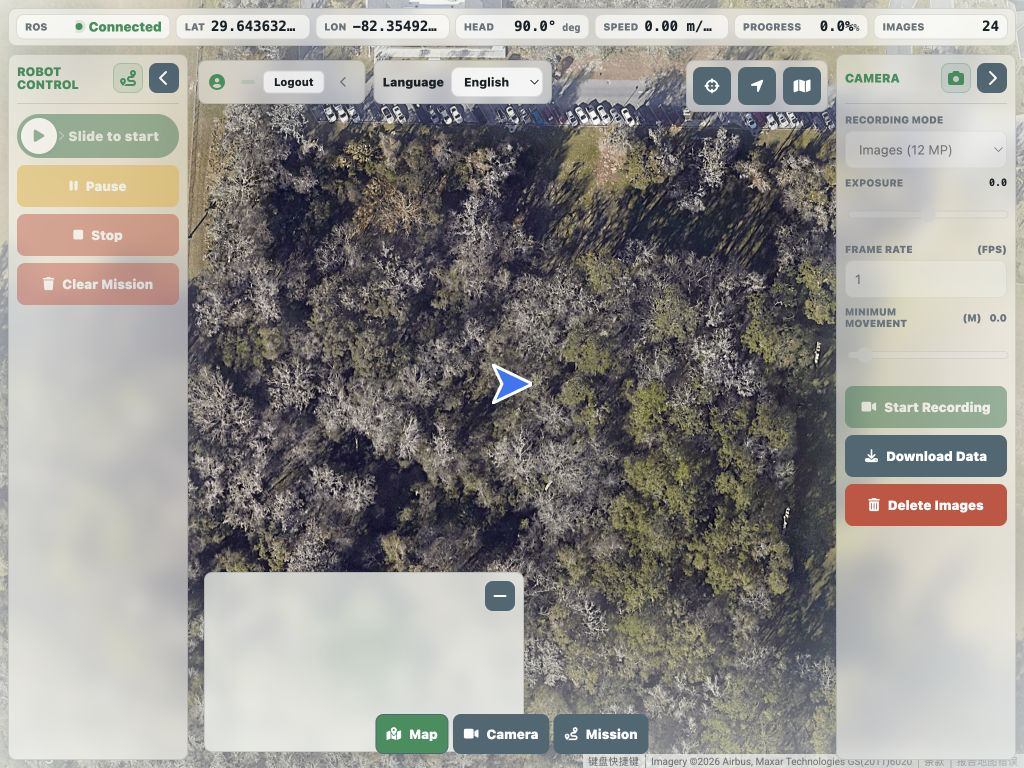
\includegraphics[keepaspectratio,alt={MARS navigation Map page at 1024 by 760 pixels with status bar and robot controls}]{assets/mars-console-map.png}}
\caption{Before planning, require ROS Connected, plausible position and
heading, current RTK localization, live camera, CAN communication, and a
stationary robot in Hold.}
\end{figure}

\subsubsection{A · Prepare localization and
system}\label{a-prepare-localization-and-system}

\begin{enumerate}
\tightlist
\item
  Place the RTK base at its recorded point with clear sky. Attach its
  GNSS and RTK LoRa antennas, power it, and open
  \texttt{mars\_gnss\_base.local}. Verify Fixed Location or complete the
  approved survey; do not move the base afterward.
\item
  Verify the base correction output. The base and rover RTK LoRa
  settings must match each other and must remain separated from the RC
  LoRa settings.
\item
  Complete the \textbf{Common readiness procedure}. Confirm the rover
  receives 5 V and CAN from its power-hub 5 V CAN port and reports an
  approved RTK fix, fresh correction age, stable heading, acceptable
  accuracy, and solution status OK.
\item
  Confirm the navigation controller receives operating power/Ethernet
  from the PoE switch and uses its assigned power-hub 5 V CAN
  connection. Configure the operating phone for simultaneous robot Wi-Fi
  and cellular Internet according to \hyperref[nav-internet]{Robot Wi-Fi
  + cellular Internet}. Require web access, loaded Google map tiles,
  live camera, current map position, and no service fault.
\item
  Manually position the robot at a safe mission start if needed. Return
  to Hold, center the joystick, verify zero motion, and keep UVC
  Off/Disarmed.
\end{enumerate}

\subsubsection{B · Create and review the
mission}\label{b-create-and-review-the-mission}

\begin{figure}
\centering
\pandocbounded{
\includegraphics[keepaspectratio,alt={Navigation webpage controls for drawing field border first row generating rows and editing waypoints}]{assets/manual-planning-buttons.pdf}}
\caption{Draw the permitted field first, then define row direction and
generate or manually add waypoints.}
\end{figure}

\begin{enumerate}
\setcounter{enumi}{5}
\tightlist
\item
  Open the approved navigation address, sign in as Operator, and select
  \textbf{Claim Control}. Confirm no other operator is issuing commands.
\item
  Select \textbf{Mission}, then \textbf{Draw Border}. Tap at least three
  points around the permitted operating area. Keep the boundary inside
  safe terrain and away from ditches, roads, people, structures, water,
  steep slopes, and unverified crop clearance.
\item
  Select \textbf{Draw First Row} and choose points A and B to set the
  row direction. Enter row count, spacing, and a conservative default
  speed, then select \textbf{Generate}.
\item
  Inspect every straight segment, turn, row transition, waypoint order,
  start direction, and final stop. Drag or edit points only while
  navigation is inactive. Add actions such as Take Photo or Stop \& Wait
  only where the physical surroundings allow them.
\item
  Open each critical waypoint and verify latitude, longitude, speed, XY
  tolerance, yaw tolerance, action, and hold time. Save the approved
  mission file for records.
\item
  Select \textbf{Upload Mission}. Review the confirmation values and
  keep the geofence enabled. Confirm the robot marker begins inside the
  permitted boundary and the uploaded waypoint count/order matches the
  reviewed plan.
\end{enumerate}

\subsubsection{C · Start, supervise, pause, and
finish}\label{c-start-supervise-pause-and-finish}

\begin{figure}
\centering
\pandocbounded{
\includegraphics[keepaspectratio,alt={Navigation webpage controls for upload slide to start pause resume stop and mission management}]{assets/manual-navigation-buttons.pdf}}
\caption{Uploading does not move the robot. Motion begins only after the
robot reports Auto and the deliberate Slide to Start gesture is
completed.}
\end{figure}

\begin{figure}
\centering
\pandocbounded{
\includegraphics[keepaspectratio,alt={Illustrated autonomous mission sequence from readiness through execute supervision pause and completion}]{assets/navigation-operation-guide.pdf}}
\caption{Monitor the physical robot and the console together; neither
view is sufficient by itself.}
\end{figure}

\begin{enumerate}
\setcounter{enumi}{11}
\tightlist
\item
  Walk or otherwise inspect the route, clear the operating area, brief
  spotters, and place the emergency-stop operator where the robot and
  access points remain observable.
\item
  Change the robot mode to \textbf{Auto} using the selected remote
  controller. Follow the applicable \hyperref[remote-operation]{Single
  Joystick Remote Controller} or \hyperref[custom-operation]{Dual
  Joystick Remote Controller} manual for its physical controls. Wait for
  both the remote controller and webpage to report Auto; the displayed
  mode is the confirmation.
\item
  On the webpage, complete \textbf{Slide to Start}. Verify the first
  movement is slow and directed toward waypoint 1. Press the emergency
  stop for movement in the wrong direction or any immediate hazard.
\item
  Continuously compare the physical robot with the map marker, active
  waypoint, driven track, heading, speed, RTK state/correction age,
  covariance/localization status, CAN state, battery, camera, geofence,
  and messages.
\item
  For a controlled pause, select webpage \textbf{Pause} or change the
  robot mode to \textbf{Auto Pause} using the selected remote
  controller. Confirm the robot physically stops, the webpage reports
  Paused, and the displayed robot mode is Auto Pause. Identify and
  correct the pause reason before continuing.
\item
  Resume only when the path is clear, localization is valid, the robot
  is inside the geofence, and the cause has been corrected. Select
  webpage \textbf{Resume} or change the robot mode from Auto Pause back
  to \textbf{Auto} using the selected remote controller; then verify
  Auto and the next physical motion.
\item
  End autonomous navigation in either of two ways: select webpage
  \textbf{Stop}, or change the robot from Auto to \textbf{Manual} or
  \textbf{Hold} with the handheld. A change to Manual or Hold
  automatically stops the active navigation mission.
\item
  After the mode change or webpage Stop, verify physical motion and
  commanded speed are zero and the console no longer reports Navigating.
  For joystick control, confirm Manual before moving the joystick;
  choose Hold when no manual movement is required.
\item
  At the final waypoint, verify the webpage reports completion,
  commanded speed is zero, and the robot is physically stopped. Select
  Hold and release web control or log out.
\item
  Save the mission result, images/videos, driven track, alarms, pauses,
  RTK quality, and any route corrections. Then follow
  \hyperref[operations-shutdown]{System shutdown}.
\end{enumerate}

\textbf{Autonomous operation is complete when:} mission execution is
stopped or completed, speed command and physical motion are zero, the
robot is in Hold, web control is released, UVC remains Off/Disarmed
unless separately authorized, and mission records are saved.

\subsection{System shutdown}\label{operations-shutdown}

\begin{figure}
\centering
\pandocbounded{
\includegraphics[keepaspectratio,alt={Complete system operations returning to Hold Off Disarmed and power isolated}]{assets/system-operations-overview.pdf}}
\caption{Every operation returns through the same safe end state before
power is removed.}
\end{figure}

\begin{enumerate}
\tightlist
\item
  Park on stable ground away from traffic, people, animals, standing
  water, and combustible material.
\item
  Stop the mission if active, center the joystick, select Hold, and
  verify zero command and zero physical motion.
\item
  Command UVC All Off, verify all six relay channels and four physical
  lamps Off, Disarm, and open the physical UVC disconnect.
\item
  Release navigation web control and save required mission, treatment,
  image/video, fault, and maintenance records.
\item
  Switch off the robot using the approved order. Remember that the main
  contactor and stored electrical energy require the specified
  discharge/lockout procedure before service.
\item
  Switch off handhelds, base equipment, and accessories as the field
  plan requires. Protect antennas/connectors and store or charge
  batteries according to the maintenance procedure.
\item
  Walk around the stopped system. Check for heat, odor, damage, loose
  cables, crop entanglement, lamp damage, fluid ingress, or a fault
  requiring tag-out.
\end{enumerate}

\chapter{Maintenance}\label{maintenance-1}

\protect\phantomsection\label{maintenance}
\section{System maintenance schedule}\label{system-maintenance-schedule}

{\def\LTcaptype{none} % do not increment counter
\begin{longtable}[]{@{}
  >{\raggedright\arraybackslash}p{(\linewidth - 2\tabcolsep) * \real{0.5000}}
  >{\raggedright\arraybackslash}p{(\linewidth - 2\tabcolsep) * \real{0.5000}}@{}}
\toprule\noalign{}
\begin{minipage}[b]{\linewidth}\raggedright
When
\end{minipage} & \begin{minipage}[b]{\linewidth}\raggedright
Work
\end{minipage} \\
\midrule\noalign{}
\endhead
\bottomrule\noalign{}
\endlastfoot
Before every use & Inspect cases, controls, the three Dual Joystick
Remote Controller antennas, wheels, steering, batteries, eight side
ports, cables, emergency stop, GPS mounts, navigation
controller/camera/PoE, lamps, guards, warning indicators and every
installed safety device; verify Hold and UVC Off. \\
After every use & Hold, All Off, Disarm, physical disconnect, approved
power-down, clean lenses/displays, record faults, store/charge batteries
correctly. \\
Weekly or after transport & Check joystick calibration, fasteners,
antenna cables, contactor, steering home, PoE switch,
navigation-controller cooling/storage, camera focus, base mount, rover
correction, and the UVC relay\textquotesingle s 5 V power/CAN connection
and fail-safe. \\
After software/configuration change & Record new version/settings;
restrain robot; test emergency stop, Hold, directions, link loss, CAN,
GPS, mission Pause/Resume, geofence, video, All Off, Disarm, and
heartbeat shutdown. \\
\end{longtable}
}

\protect\phantomsection\label{emergency}
\section{Emergency actions}\label{emergency-actions}

\begin{manualdanger}

\textbf{Unsafe robot movement:} release controller, press the physical
emergency stop, keep people away, and disconnect power only when safe.

\end{manualdanger}

\begin{manualdanger}

\textbf{Possible UV-C exposure:} do not enter immediately. Command All
Off if available, use the physical UVC disconnect, follow site
exposure/emergency procedures, and have the system inspected before
reuse.

\end{manualdanger}

\begin{manualwarning}

\textbf{Lost radio or webpage:} do not assume the robot or lamps are
off. Use physical safety controls and verify the machine directly from a
safe location.

\end{manualwarning}

\begin{enumerate}
\tightlist
\item
  Protect people first; use the physical emergency control.
\item
  Do not reset or re-arm until the cause is identified.
\item
  Inspect actual motor, relay, lamp, and indicator state.
\item
  Record the event and complete a restrained functional test before
  returning to service.
\end{enumerate}

\protect\phantomsection\label{system-engineer}
\section{Entire robot system: field-engineer
commissioning}\label{entire-robot-system-field-engineer-commissioning}

Commission from the physical layer upward. Do not troubleshoot
application software until power, grounding, antenna, termination, and
bus wiring are verified.

{\def\LTcaptype{none} % do not increment counter
\begin{longtable}[]{@{}
  >{\raggedright\arraybackslash}p{(\linewidth - 2\tabcolsep) * \real{0.5000}}
  >{\raggedright\arraybackslash}p{(\linewidth - 2\tabcolsep) * \real{0.5000}}@{}}
\toprule\noalign{}
\begin{minipage}[b]{\linewidth}\raggedright
Stage
\end{minipage} & \begin{minipage}[b]{\linewidth}\raggedright
Acceptance criteria
\end{minipage} \\
\midrule\noalign{}
\endhead
\bottomrule\noalign{}
\endlastfoot
1 · Mechanical & Fasteners secure; wheels/steering free; antennas,
camera, and GPS mounts rigid; four UVC fixtures, shielding, and access
controls complete. \\
2 · Power & Correct polarity/voltage; batteries healthy; four
battery-power ports and four CAN ports labeled; contactor and branch
protection correct; PoE switch powered; navigation controller has no
undervoltage; UVC supply independently disconnectable. \\
3 · Safety & Physical E-stop stops motion independently; both UVC groups
Off/Disarm; PPE, interlocks, and indicators verified. \\
4 · CAN & Every side CAN port verified as 12 V, GND, CANH, CANL;
\textbf{500 kbit/s}; correct termination; unique node IDs; controllers,
motors, batteries, GPS, navigation controller, and relay online without
bus errors. \\
5 · Radio & RC endpoints match each other; RTK endpoints match each
other; RC and RTK settings are separated to prevent interference; normal
RSSI and safe link-loss response. \\
6 · Manual motion & Hold at startup; centered zero; correct
drive/steering direction; feedback follows low-speed command. \\
7 · GPS & Base valid/fixed; fresh corrections; rover RTK; position
delivered through CAN and ROS. \\
8 · Navigation & PoE switch/module, navigation-controller services, ROS,
CAN, CSI camera, and video healthy; mission/geofence/Pause/Resume/photo
and safety gates verified. \\
9 · UVC & Left-side/top-left Group A and right-side/top-right Group B
labels verified; requested/applied/physical states agree; heartbeat/CAN
emergency shutdown and warning confirmation verified. \\
10 · Records & Firmware, commits, node IDs, port pinout, radio/group
mapping, lamp hours, base coordinates, calibration, test results, and
backups recorded. \\
\end{longtable}
}

\subsection{Engineering handover
package}\label{engineering-handover-package}

\begin{itemize}
\tightlist
\item
  Controller, robot, relay, base, and rover firmware versions and
  approved binaries.
\item
  Navigation-controller OS image, Raspberry Pi 5/CSI/PoE hardware
  record, \texttt{video-stream} commit, build/dependency record, and
  installed service files.
\item
  Robot-side power/CAN port schedule, contactor and protection diagram,
  \textbf{500 kbit/s} CAN setting, node/COB-ID schedule, bus diagram,
  and termination locations.
\item
  UVC Group A/B channel schedule, fixture/ballast diagram, four lamp
  positions, hours, approved dose/speed table, and radiometer
  calibration record.
\item
  Separate RC and RTK radio settings/channel plan; store passwords
  separately under site policy.
\item
  Base coordinates/survey method, antenna offsets, and navigation
  geometry parameters.
\item
  Safety-validation record for E-stop, PPE, interlocks, UVC fail-safe,
  link loss, command timeout, geofence, and localization pause.
\end{itemize}

\end{document}
